\PassOptionsToPackage{unicode=true}{hyperref} % options for packages loaded elsewhere
\PassOptionsToPackage{hyphens}{url}
%
\documentclass[11pt,]{book}
\usepackage{lmodern}
\usepackage{amssymb,amsmath}
\usepackage{ifxetex,ifluatex}
\usepackage{fixltx2e} % provides \textsubscript
\ifnum 0\ifxetex 1\fi\ifluatex 1\fi=0 % if pdftex
  \usepackage[T1]{fontenc}
  \usepackage[utf8]{inputenc}
  \usepackage{textcomp} % provides euro and other symbols
\else % if luatex or xelatex
  \usepackage{unicode-math}
  \defaultfontfeatures{Ligatures=TeX,Scale=MatchLowercase}
\fi
% use upquote if available, for straight quotes in verbatim environments
\IfFileExists{upquote.sty}{\usepackage{upquote}}{}
% use microtype if available
\IfFileExists{microtype.sty}{%
\usepackage[]{microtype}
\UseMicrotypeSet[protrusion]{basicmath} % disable protrusion for tt fonts
}{}
\IfFileExists{parskip.sty}{%
\usepackage{parskip}
}{% else
\setlength{\parindent}{0pt}
\setlength{\parskip}{6pt plus 2pt minus 1pt}
}
\usepackage{hyperref}
\hypersetup{
            pdftitle={The Political Economy of National Oil Companies as International Investors},
            pdfauthor={David Tingle},
            pdfborder={0 0 0},
            breaklinks=true}
\urlstyle{same}  % don't use monospace font for urls
\usepackage[margin=1.5in]{geometry}
\usepackage{color}
\usepackage{fancyvrb}
\newcommand{\VerbBar}{|}
\newcommand{\VERB}{\Verb[commandchars=\\\{\}]}
\DefineVerbatimEnvironment{Highlighting}{Verbatim}{commandchars=\\\{\}}
% Add ',fontsize=\small' for more characters per line
\usepackage{framed}
\definecolor{shadecolor}{RGB}{248,248,248}
\newenvironment{Shaded}{\begin{snugshade}}{\end{snugshade}}
\newcommand{\AlertTok}[1]{\textcolor[rgb]{0.94,0.16,0.16}{#1}}
\newcommand{\AnnotationTok}[1]{\textcolor[rgb]{0.56,0.35,0.01}{\textbf{\textit{#1}}}}
\newcommand{\AttributeTok}[1]{\textcolor[rgb]{0.77,0.63,0.00}{#1}}
\newcommand{\BaseNTok}[1]{\textcolor[rgb]{0.00,0.00,0.81}{#1}}
\newcommand{\BuiltInTok}[1]{#1}
\newcommand{\CharTok}[1]{\textcolor[rgb]{0.31,0.60,0.02}{#1}}
\newcommand{\CommentTok}[1]{\textcolor[rgb]{0.56,0.35,0.01}{\textit{#1}}}
\newcommand{\CommentVarTok}[1]{\textcolor[rgb]{0.56,0.35,0.01}{\textbf{\textit{#1}}}}
\newcommand{\ConstantTok}[1]{\textcolor[rgb]{0.00,0.00,0.00}{#1}}
\newcommand{\ControlFlowTok}[1]{\textcolor[rgb]{0.13,0.29,0.53}{\textbf{#1}}}
\newcommand{\DataTypeTok}[1]{\textcolor[rgb]{0.13,0.29,0.53}{#1}}
\newcommand{\DecValTok}[1]{\textcolor[rgb]{0.00,0.00,0.81}{#1}}
\newcommand{\DocumentationTok}[1]{\textcolor[rgb]{0.56,0.35,0.01}{\textbf{\textit{#1}}}}
\newcommand{\ErrorTok}[1]{\textcolor[rgb]{0.64,0.00,0.00}{\textbf{#1}}}
\newcommand{\ExtensionTok}[1]{#1}
\newcommand{\FloatTok}[1]{\textcolor[rgb]{0.00,0.00,0.81}{#1}}
\newcommand{\FunctionTok}[1]{\textcolor[rgb]{0.00,0.00,0.00}{#1}}
\newcommand{\ImportTok}[1]{#1}
\newcommand{\InformationTok}[1]{\textcolor[rgb]{0.56,0.35,0.01}{\textbf{\textit{#1}}}}
\newcommand{\KeywordTok}[1]{\textcolor[rgb]{0.13,0.29,0.53}{\textbf{#1}}}
\newcommand{\NormalTok}[1]{#1}
\newcommand{\OperatorTok}[1]{\textcolor[rgb]{0.81,0.36,0.00}{\textbf{#1}}}
\newcommand{\OtherTok}[1]{\textcolor[rgb]{0.56,0.35,0.01}{#1}}
\newcommand{\PreprocessorTok}[1]{\textcolor[rgb]{0.56,0.35,0.01}{\textit{#1}}}
\newcommand{\RegionMarkerTok}[1]{#1}
\newcommand{\SpecialCharTok}[1]{\textcolor[rgb]{0.00,0.00,0.00}{#1}}
\newcommand{\SpecialStringTok}[1]{\textcolor[rgb]{0.31,0.60,0.02}{#1}}
\newcommand{\StringTok}[1]{\textcolor[rgb]{0.31,0.60,0.02}{#1}}
\newcommand{\VariableTok}[1]{\textcolor[rgb]{0.00,0.00,0.00}{#1}}
\newcommand{\VerbatimStringTok}[1]{\textcolor[rgb]{0.31,0.60,0.02}{#1}}
\newcommand{\WarningTok}[1]{\textcolor[rgb]{0.56,0.35,0.01}{\textbf{\textit{#1}}}}
\usepackage{longtable,booktabs}
% Fix footnotes in tables (requires footnote package)
\IfFileExists{footnote.sty}{\usepackage{footnote}\makesavenoteenv{longtable}}{}
\usepackage{graphicx,grffile}
\makeatletter
\def\maxwidth{\ifdim\Gin@nat@width>\linewidth\linewidth\else\Gin@nat@width\fi}
\def\maxheight{\ifdim\Gin@nat@height>\textheight\textheight\else\Gin@nat@height\fi}
\makeatother
% Scale images if necessary, so that they will not overflow the page
% margins by default, and it is still possible to overwrite the defaults
% using explicit options in \includegraphics[width, height, ...]{}
\setkeys{Gin}{width=\maxwidth,height=\maxheight,keepaspectratio}
\setlength{\emergencystretch}{3em}  % prevent overfull lines
\providecommand{\tightlist}{%
  \setlength{\itemsep}{0pt}\setlength{\parskip}{0pt}}
\setcounter{secnumdepth}{5}
% Redefines (sub)paragraphs to behave more like sections
\ifx\paragraph\undefined\else
\let\oldparagraph\paragraph
\renewcommand{\paragraph}[1]{\oldparagraph{#1}\mbox{}}
\fi
\ifx\subparagraph\undefined\else
\let\oldsubparagraph\subparagraph
\renewcommand{\subparagraph}[1]{\oldsubparagraph{#1}\mbox{}}
\fi

% set default figure placement to htbp
\makeatletter
\def\fps@figure{htbp}
\makeatother

\usepackage{booktabs}
\usepackage[ style=chicago-authordate,
	backend=bibtex,
	natbib=true,
	sorting=nyt,
	doi=false,
	isbn=false,
	url=false,
	eprint=false,
	maxbibnames=100,
	maxcitenames=2,
	]{biblatex}
	\AtEveryCitekey{\UseBibitemHook}
\newbibmacro{string+doiurlisbn}[1]{%
  \iffieldundef{doi}{%
    \iffieldundef{url}{%
      \iffieldundef{isbn}{%
        \iffieldundef{issn}{%
          #1%
        }{%
          \href{http://books.google.com/books?vid=ISSN\thefield{issn}}{#1}%
        }%
      }{%
        \href{http://books.google.com/books?vid=ISBN\thefield{isbn}}{#1}%
      }%
    }{%
      \href{\thefield{url}}{#1}%
    }%
  }{%
    \href{http://dx.doi.org/\thefield{doi}}{#1}%
  }%
}
\DeclareFieldFormat{title}{\usebibmacro{string+doiurlisbn}{\mkbibemph{#1}}}
\DeclareFieldFormat[article,incollection]{title}%
    {\usebibmacro{string+doiurlisbn}{\mkbibquote{#1}}}
\usepackage{setspace}
\doublespacing
\usepackage{booktabs}
\usepackage{longtable}
\usepackage{array}
\usepackage{multirow}
\usepackage{wrapfig}
\usepackage{float}
\usepackage{colortbl}
\usepackage{pdflscape}
\usepackage{tabu}
\usepackage{threeparttable}
\usepackage{threeparttablex}
\usepackage[normalem]{ulem}
\usepackage{makecell}
\usepackage{xcolor}

\title{The Political Economy of National Oil Companies as International Investors}
\author{David Tingle}
\date{Last Edited: 2020-06-25}

\begin{document}
\maketitle

{
\setcounter{tocdepth}{1}
\tableofcontents
}
\hypertarget{overview}{%
\chapter*{Overview}\label{overview}}
\addcontentsline{toc}{chapter}{Overview}

National Oil Companies (NOCs) were initially built to give states some degree of control over their domestic hydrocarbon resources, but many of them have now acquired assets and established subsidiaries outside of their home state. This dissertation adresses three key questions related to this phenomenon:

\begin{itemize}
\tightlist
\item
  \textbf{First, how does NOC internationalization vary?} NOCs are some of the largest economic entities in existence today. Their international activities often receive high levels of publicity and scrutiny. When Saudi Arabia's Aramco acquires an asset outside of the Kingdom, the Crown Prince is often involved in the announcement and firm executives are accompanied by the highest levels of the diplomatic corps. Despite this significance, however, we don't have a broad or systematic understanding of these international activities. For example, we don't currently know much about which firms have a large international presence and which are limited to domestic operations, which countries are the most common investment targets, whether firms invest in raw resource assets or downstream value chain assets, and so on. The goal of this chapter is to introduce and then utilize an approach to measuring internationalization based on the subsidiaries NOCs establish outside their home state.
\item
  \textbf{Second, why are some NOCs highly internationalized and others aren't?} This question is at the core of the current literature on NOC internationalization, but good answers to it are limited by a relatively sparse data environment and by a lack of attention to comprehensive theory development. This chapter addresses the question head on by using graphical causal modelling to develop and then evaluate a theory of NOC internationalization that unifies and builds on exisitng work on the subject.
\item
  \textbf{Third, what are the political consequences of NOC internationalization?} The suggestion that NOC activities -- whether they be domestic or international -- can be tied up in politics in meaningful ways is likely uncontroversial. Systematically investigating the political implications of this activity, however, is more challenging. This chapter makes two moves to improve our understanding of this important but under-researched topic. First, it takes a structured approach to definining the range and shape of what these political implications could be, and explores the NOC internationalization data to determine whether patterns in NOC subsidiary networks are consistent with these expectations. Second, it utilizes state-space structural models to investigate the causal impact of internationalization over time on key political outcomes of interest.
\end{itemize}

In addressing these questions together as part of a unified project, this research sheds light on a set of integral but under-theorized institutions, NOCs, at the centre of contemporary state capitalism and the political economy of resource wealth.

\hypertarget{paper1}{%
\chapter{What is NOC Internationalization?}\label{paper1}}

\hypertarget{intro01}{%
\section{Introduction}\label{intro01}}

In December of 2014, the Russian government engaged a drastic interest rate hike in the hopes of defending the ruble. There are a number of reasons for the Russian currency's precipitous decline in recent months --- these include the stock market cost of military adventurism in Ukraine and the general decline in oil prices. The drop in the ruble's value in mid-December, however, has been linked by observers to an ``opaque deal involving the central bank and the state-controlled oil company, Rosneft'' (Kramer \protect\hyperlink{ref-kramer_russias_2014}{2014}). The oil company, \emph{The New York Times} goes on to report, ``had been clamoring for months for a government bailout to refinance debt the company ran up while making acquisitions when oil prices were high.''

A little earlier in the year, news broke in Canada that a major corruption and embezzlement scandal within the state-owned China National Petroleum Corporation (CNPC) would slow a project in Alberta's Athabasca oil sands involving its subsidiary PetroChina (Jones \protect\hyperlink{ref-jones_china_2014}{2014}). Political intrigue at home became a major story in the resource-rich Canadian province. More broadly, Chinese state-owned firms are under intense scrutiny for the declining value of their recent purchases in the Albertan oil sands. China isn't the only foreign state investing in the oil sands: all of the top ten foreign investment deals in the Canadian energy industry have been made by state-owned firms, and six of those involved a non-Chinese state-owned enterprise.\footnote{(``The Largest Foreign Investment Deals Made in the Canadian Energy Industry'' \protect\hyperlink{ref-noauthor_largest_2014}{2014}).}

Risky investments and corruption intrigue are part of the story for all types of business; what these stories capture, anecdotally at least, are some of the complications of state-ownership over large economic entities. They also hint at an increasingly-important underlying phenomena: the international exposure of Rosneft and PetroChina are specific illustrations of the international investment and activity engaged in by state-owned energy firms (SOEs).

These anecdotes distill key themes this research aims to investigate empirically. At the core of each is the efforts of a state-owned oil company to acquire an international asset. While in these illustrative stories this attempt was ultimately unsuccessful, NOCs have in fact been active players in the international economy, buying and selling assets at all points in the oil \& gas value chain. Some, but certainly not all, NOCs have made efforts to grow internationally. The observable variation in this process of internationalization, and explanations as to its origins and features, are at the core of this study. What is NOC internationalization? How extensive is it? How does it differ from the internationalization pursued by non-state-owned energy firms?

The second key theme these anecdotes express is that this process of internationalization can have a highly salient, even controversial, political component to it. Large cross-border acquisitions always have at least the potential to be politically charged; this is especially true when the acquiring entity is intrinsically linked to a foreign government. Even the potential for political influence regularly raises hackles. Worried observers and regulators may not always be able to explicitly define the nature of their concern about this state influence, but they acknowledge and act on the basis of it nonetheless. This political component deserves careful empirical attention. The investment activity of SOEs is a significant element in their already well established identities as international political actors. Oil \& gas CEOs, energy ministers, and top regulatory officials feature prominently in the daily record of global politics. While the best known brands in international energy are private multinationals --- Royal Dutch Shell, BP, Exxon Mobil --- firms owned by state actors wield substantial influence. SOEs occupy 7 of the top 10 spots in Forbes' 2019 of largest oil \& gas firms; the top three spots are all held by SOEs. The contemporary reality is that the majority of global fossil fuels are produced by large firms owned by the state. We think of these firms for the most part as sellers, supplying less well-endowed states with the raw materials integral to building and sustaining a modern economy, but they are increasingly active as buyers and investors as well. This activity is a critical component of the international economic system, and has critically important international political consequences.

Addressing questions about NOC internationalization is important. However, our ability to systematically understand this process of NOC internationalization, and make sense of its political salience, has to date been hampered by a lack of good data on the subject. Internationalization is in fact an accumulation of specific acquisitions, mergers, and subsidiary creation events spread across a diverse set of internationalizing and target entities. Transactions of this nature are difficult to capture, especially when they occur in jurisdictions with less stringent reporting and filing regulations than the United States or Western Europe.

In this paper I introduce a new dataset of internationalization in the energy sector, one that focuses on the corporate hierarchies of oil \& gas firms.\footnote{Collected using Standard \& Poor's \href{http://marketintelligence.spglobal.com}{Capital IQ financial Database}.} Rather than focusing on transactions, this dataset exploits the detailed corporate hierarchy information that financial databases have accumulated over time on major economic entities. This dataset captures the first order subsidiaries of all NOCs, and a sample of the most important privately owned (or publicly traded) oil \& gas firms globally. These data capture internationalization in a global network of parent and subsidiary relationships.

These data represent a significant addition to empirical efforts to capture and analyze NOC internationalization, pursued in recent years by researchers at the intersection of political economy and business studies. Researchers have addressed the substantive questions at hand with a variety of empirical approaches. Several have pursued within-country analyses leveraging detailed firm-level data to address questions of internationalization within the context of a specific state (eg. Bass and Chakrabarty \protect\hyperlink{ref-bass_resource_2014}{2014}; Cui and Jiang \protect\hyperlink{ref-cui_state_2012}{2012}; Knutsen, Rygh, and Hveem \protect\hyperlink{ref-knutsen_does_2011}{2011}; Li, Cui, and Lu \protect\hyperlink{ref-li_varieties_2014}{2014}). Others have utilized qualitative methods to enable theory-development in the context of a few key cases (eg. Jones Luong and Sierra \protect\hyperlink{ref-jones_luong_domestic_2015}{2015}). A few studies leverage transaction-level mergers and acquisitions data to enable cross-national analysis (Cheon \protect\hyperlink{ref-cheon_developing_2019}{2019}; Clò, Fiorio, and Florio \protect\hyperlink{ref-clo_targets_2016}{2016}). There are benefits and disadvantages to each of these empirical approaches; a more complete discussion of how the new data introduced in this chapter relate to existing datasets is undertaken in section (\ref{approach01}).

Using these data, we develop a set of novel findings that improve or understanding of NOC internationalization.

\begin{itemize}
\tightlist
\item
  The majority of NOCs have acquired or established at least one international international subsidiary; 80\% of NOC subsidiaries are owned by 10\% of iNOCs.
\item
  NOCs that have internationalized have done so in a set of discrete and identifiable patterns, allowing us to generate a typology of NOC internationalization
\item
  NOC internationalization differs systematically from IOC internationalization: NOCs establish an international subsidiary network in politically-similar, geographically adjacent states.
\item
  NOCs are less likely than IOCs to pursue JVs or other shared partnerships, preferring wholly-owned vehicles
\item
  NOCs are just as likely to acquire or establish subsidiaries for resource extraction as for other prospects down the energy value chain, such as refining or distribution.
\end{itemize}

Together, these findings represent a significant improvement in our foundational understanding of how NOCs operate across borders in the contemporary economy. NOCs are some of the most materially significant economic entities operating today: they control X\% of known oil \& gas reserves, and 8/10 of the Fortune 500 2018 list. Establishing the empirical contours of how they exist as international actors is an essential part of properly accounting for their role in theories of economic nationalism, globalization, foreign direct investment flows, and domestic economic and political development (resource-influenced or otherwise). From a political economy perspective, the case can be made that contemporary state capitalism and economic nationalism are under-theorized. A better empirical understanding of some of the most important entities in this context is an essential part of rectifying that gap. A further discussion of these points is developed in Section \ref{conclusion01}.

This chapter proceeds as follows. In the next section (\ref{motiv01}) we motivate this research by discussing the state of the literature on NOC internationalization. While some political scientists are investigating this problem set, the bulk of contemporary work on the international dimensions of state-ownership lie in business studies. This relative neglect from political scientists is unwarranted, we argue, and a renewed focus stands as a nice complement to existing comparative strands of research. We also spend some time motivating the empirical approach taken in this paper in light of existing efforts to understand these phenomena.

Section \ref{approach01} introduces our dataset more fully. We discuss the data collection method, address specific areas of improvement over existing or complementary datasets, and conduct some preliminary exploratory analysis to establish a clear basis for proceeding.

Section \ref{analysis01} utilizes the dataset introduced in the preceding section to improve our understanding of NOC internationalization along a number of complementary empirical (albeit descriptive rather than strictly inferential) lines. It also investigates a central question: does NOC status has a substantive and statistically significant relationship with subsidiary political affinity? In order to test this hypothesis, we leverage state dyad ideal points data coded by Bailey, Strezhnev, and Voeten (\protect\hyperlink{ref-bailey_estimating_2017}{2017}). A more complete discussion of these data is provided in the empirical approach section.

The concluding section (\ref{conclusion01}) discusses the implications, as well as the limitations, of this research. It also explicitly connects this research with other salient lines of inquiry, several of which are pursued in distinct chapters within this study.

\hypertarget{motiv01}{%
\section{Motivation}\label{motiv01}}

This section has three primary objectives. First, it provides a brief introduction to national oil companies (NOCs) and situates them within existing political economy and business studies research, touching on general approaches but focusing in particular on the studies that aim to improve our understanding of internationalization in particular. In this discussion, our aim is to clearly establish the importance of NOC internationalization as an area of study for political economists. Second, as part of this literature review, we aim to establish the state of empirical research into the NOC internationalization as transparently as possible, establishing the need for and value of the novel data this paper introduces in the subsequent section. Third, this section introduces a number of open empirical questions concerning NOC internationalization that have to this point not been adequately addressed. These questions form the basis for the analysis developed in Section \ref{analysis01}.

\hypertarget{what-are-national-oil-companies}{%
\subsection{What are National Oil Companies?}\label{what-are-national-oil-companies}}

National Oil Companies (NOCs) are firms that operate in the hydrocarbon sector and are wholly or partially owned by the state.\footnote{The cut-point for minority state ownership is 30\% state ownership (such as Italy's ENI). Most NOCs are 100\% state-owned. NOCs are a specific kind of state-owned enterprise (SOE).} NOCs are geographically dispersed, though they are more dominant in some regions than in others. There are 88 NOCs currently in operation.

NOCs are generally primarily responsible for the stewardship and development of domestic oil and gas reserves. Out of the top 10 countries raked by proven crude oil reserves, Canada is the only state without an NOC.\footnote{\href{https://www.eia.gov/beta/international/data/browser/\#/?pa=0000000000000000000008\&c=ruvvvvvfvtvnvv1urvvvvfvvvvvvfvvvou20evvvvvvvvvnvvuvo\&ct=0\&tl_id=5-A\&vs=INTL.57-6-AFG-BB.A\&cy=2018\&vo=0\&v=H\&start=1980}{U.S. Energy Information Administration, 2017 Statistics}. Canada established a wholly owned oil \& gas crown corporation, Petro Canada, in 1975, and initiated privatization in 1990. The government divested its remaining 19\% stake in 2004, and Petro Canada is now owned by Suncor Energy.} NOCs can take primary responsibility for resource extraction (drilling, etc.) though some also contract these activities out to third parties (other large oil \& gas firms). Many NOCs also operate at other points in the hydrocarbon value chain, including refining, transportation (shipping and pipelines), and even consumer sales (Mexico's PEMEX, for instance, has a national chain of vehicle gas stations). NOCs are not restricted to operating in the oil \& gas sectors, either: some own subsidiaries or investment arms that operate in very different commercial sectors such as electricity grid management, or real estate. NOCs can be the most significant contributor to the economy and the largest employer, as in the case of Saudi Arabia's Saudi Aramco; others feature regularly in state-to-state diplomatic exchanges, as in the case of Russia's Gazprom. Others invest heavily in brand placement, such as Malaysia's Petronas and its Formula One sponsorship.

Just as NOCs vary in terms of their operations and corporate focus, they vary with respect to the practicalities of state-ownership as well. Many operate under the purview of a Ministry of Energy, where ultimate authority for the firm's operations rests on an elected (or appointed) government minister. Others slot into a bureaucratic function and are insulated from elected decision-makers. Still others see their boards and leadership positions staffed by close associates or family members of a ruling clan, or serve as patronage opportunities for loyalists. States may have an interest in actively managing the affairs of the firm, or may prefer to let the firm work at arms-length from political functions so that it can operate as a purely economic actor.

\hypertarget{what-do-we-know-about-nocs}{%
\subsection{What do we know about NOCs?}\label{what-do-we-know-about-nocs}}

Academic research into NOCs can be roughly grouped into four categories. First, scholarship across several disciplines has sought to address the question of why NOCs exist in the first place. The earliest of these focus on the historical genesis of NOCs as oil supply managers and evolution into production and export businesses. Many focus on explaining why states rely on state-owned firms instead of a competitive market for production and distribution (eg. Tordo \protect\hyperlink{ref-tordo_national_2011}{2011}). Recent scholarship in this vein focuses on the nationalization process that generated many NOCs (Mahdavi \protect\hyperlink{ref-mahdavi_why_2014}{2014}). Many of these studies focus on a particular region and draw comparisons across a limited set of NOCs (eg. Marcel and Mitchell \protect\hyperlink{ref-marcel_oil_2006}{2006}).

Second, a body research --- developed in particular, but not exclusively, by applied economists --- has investigated the economic activity of NOCs. Many of these studies examine and compare the efficiency and effectiveness of NOCs as economic entities, particularly in relation to non-state owned peers (eg. Hartley and Medlock III \protect\hyperlink{ref-hartley_model_2008}{2008}; Eller, Hartley, and Medlock III \protect\hyperlink{ref-eller_empirical_2011}{2011}; Thurber, Hults, and Heller \protect\hyperlink{ref-thurber_exporting_2011}{2011}; Nolan and Thurber \protect\hyperlink{ref-victor_states_2012}{2012}). A useful review of both of these first literatures, focusing on historical genesis and economic efficiency, can be found in Victor (\protect\hyperlink{ref-victor_national_2013}{2013}).

Hydrocarbons are a foundational component to modern political science\footnote{Foundational, in that canonical texts in international political economy in particular were developed to explain, in large part, political phenomena in energy policy and energy security. See Krasner (\protect\hyperlink{ref-krasner_defending_1978}{1978}), Keohane (\protect\hyperlink{ref-keohane_after_1984}{1984}), Ikenberry (\protect\hyperlink{ref-ikenberry_irony_1986}{1986}), and Ikenberry (\protect\hyperlink{ref-ikenberry_reasons_1988}{1988}).}, but political scientists have devoted limited attention to NOCs in particular. This lack of attention is surprising, given that NOCs are one of the most important institutions at the intersection of hydrocarbon wealth and the state. Some exceptions exist. Jones Luong and Sierra (\protect\hyperlink{ref-jones_luong_domestic_2015}{2015}) argue that ownership institutions --- NOCs most prominent among them --- are essential to understanding the causal process that connects hydrocarbon endowments with outcomes like economic and political development\footnote{See Losman (\protect\hyperlink{ref-losman_rentier_2010}{2010}) for another example, focused on the Middle East}. Cheon, Lackner, and Urpelainen (\protect\hyperlink{ref-cheon_instruments_2014}{2014}) examine some of the ways that states can use their NOCs strategically for domestic ends, in particular by insulating domestic consumer markets from adverse trends in oil prices. Strategic concerns and political economy also feature prominently in some of the core omnibus analyses of NOCs (eg. Victor, Hults, and Thurber \protect\hyperlink{ref-victor_oil_2012}{2012}; Marcel and Mitchell \protect\hyperlink{ref-marcel_oil_2006}{2006}). Overall, however, research into NOCs continues to be marginal in political science and political economy.\footnote{A recent \emph{Annual Review of Political Science} survey on ``The Politics of Energy'', tellingly, makes no explicit references to NOCs, despite a few citations pointed towards research that focus exclusively on NOCs (Hughes and Lipscy \protect\hyperlink{ref-hughes_politics_2013}{2013}).}

This relative lack of attention extends to international relations and international political economy. While NOC internationalization has drawn some interest from the popular press,\footnote{eg. A special issue on the topic in \emph{The Economist} in 2012 (\emph{The Economist} \protect\hyperlink{ref-noauthor_new_2012}{2012}). See also (\emph{The Economist} \protect\hyperlink{ref-noauthor_leviathan_2014}{2014}).} relatively few political economists have addressed the phenomenon of NOCs expanding into international markets. The bulk of academic work in this area has been pursued by business studies scholars. This research addresses a number of key questions related to NOC internationalization. Many of these studies leverage detailed Chinese firm-level outbound foreign direct investment (FDI) data to test their hypotheses. Cui and Jiang (\protect\hyperlink{ref-cui_state_2012}{2012}) find that state ownership modifies how Chinese firms engage in FDI, in particular by increasing the degree to which these firms conform to target market institutional pressures\footnote{Meyer et al. (\protect\hyperlink{ref-meyer_overcoming_2014}{2014}) find supporting evidence for this argument.}. Liang, Ren, and Sun (\protect\hyperlink{ref-liang_anatomy_2014}{2014}) unpack state control, finding evidence that formal and informal mechanisms of control and influence have varying effects on Chinese state-owned outward FDI. Duanmu (\protect\hyperlink{ref-duanmu_state-owned_2014}{2014}) find that state-ownership may help investing firms counter the risk of expropriation through the political influence of their state owner. Pan et al. (\protect\hyperlink{ref-pan_firms_2014}{2014}) find that state ownership moderates investing firms' preference for high ownership states in favorable target markets: firms that have higher levels of state ownership (exercised through both formal and informal channels) demonstrate weaker preferences for high ownership in favorable markets (and for low ownership in less favorable markets)\footnote{A complementary analysis can be found in Ramasamy, Yeung, and Laforet (\protect\hyperlink{ref-ramasamy_chinas_2012}{2012})}. Li et al. (\protect\hyperlink{ref-li_diplomatic_2017}{2017}) examine the value of diplomatic channels in establishing international business relationships: state-owned firms with stronger ties to their home state leverage diplomatic relationships more extensively when establishing a foreign subsidiary, and will use these relationships to inform the choice of target market. Many of these research strands are usefully summarized in Buckley et al. (\protect\hyperlink{ref-buckley_retrospective_2018}{2018}).

Beyond the Chinese context, Bass and Chakrabarty (\protect\hyperlink{ref-bass_resource_2014}{2014}) find that state-owned enterprises (SOEs) focus their international investments on (and pay more for) exploration, arguing that this is primarily motivated by resource scarcity and security concerns on the home (investing) state's side of the investment. Choudhury and Khanna (\protect\hyperlink{ref-choudhury_toward_2014}{2014}) modify this standard resource dependence theory in a novel way, utilizing Indian firm-level data to find evidence that SOEs engage in internationalization to improve their strategic position and independence from other state institutions (ministries, agencies, etc.).

Li, Cui, and Lu (\protect\hyperlink{ref-li_varieties_2014}{2014}) develop (but do not empirically evaluate) an extensive set of theories focused on explaining the link between institutional variation (``varieties of state capitalism'') and outward international investment: their core contribution is in creating a typology of SOE organizational variation. Mohr, Wang, and Fastoso (\protect\hyperlink{ref-mohr_contingent_2016}{2016}) find that resource dependence isn't just a reason for state-owned firms' outward investment: international joint ventures with a state-owned party reduces the risk of joint venture dissolution as well. Musacchio and Lazzarini (\protect\hyperlink{ref-musacchio_reinventing_2014}{2014}) focus on Brazil to produce one of the most extensive and interesting recent treatments of contemporary state capitalism.

Several recent studies extend this line of inquiry into political science properly speaking. Jones Luong and Sierra (\protect\hyperlink{ref-jones_luong_domestic_2015}{2015}) focus on variation in Latin American NOCs to argue that patterns of internationalization can be explained by the interaction of two variables: the nationalization process that formed the firm in the first place, and the historical convergence of state and firm interests regarding internationalization. Meckling, Kong, and Madan (\protect\hyperlink{ref-meckling_oil_2015}{2015}) utilize Indian (and Chinese) data to argue that NOC internationalization is impacted by the balance of cooperation and conflict that exists between the state and the firm in question. Chalmers and Mocker (\protect\hyperlink{ref-chalmers_end_2017}{2017}) contest the basic view that SOEs are more risk-acceptant in their choice of investment target: they find that risk acceptance varies depending on whether the firm or the state primarily owns that risk. Finally, Cheon (\protect\hyperlink{ref-cheon_developing_2019}{2019}) leverages a cross-national dataset of NOC mergers \& acquisitions transactions to argue that domestic politics explain NOC internationalization: greater levels of partisan competition domestically reduce state tolerance for investment risk, and by extension appetite for expansion. We discuss the empirical basis for each of these studies in more detail in Section \ref{approach01}. The objective of Chapter \ref{paper2} is to directly engage with the theoretical arguments contained in this literature.

\hypertarget{noc-internationalization-opportunities-for-research}{%
\subsection{NOC internationalization: opportunities for research}\label{noc-internationalization-opportunities-for-research}}

We can draw at least three conclusions from this survey.

First, there is no good reason for the neglect of National Oil Companies in political science research. They sit in a key place, substantively and theoretically, for some of the most important topics in the field (the resource curse, energy security). As institutions, they marry political and economic influences and processes in a variety of organizational forms, and continue to be the most salient and influential evidence of robust state capitalism in the contemporary economy. When we consider their international expansion in particular, as an set of activity it is substantial enough to have made a major impact on the global market for oil \& gas, and instances of NOC investment regularly receive intense scrutiny from the popular press and from political actors themselves. Scholars in adjacent disciplines have built a robust literature explaining NOC internationalization with reference to a set of explicitly political variables of interest.

Second, our empirical understanding of NOCs, and NOC internationalization in particular, can and should be improved. The bulk of existing research, regardless of discipline is built on single-country analyses or small-n case comparisons. As such, the generalizability of many of the arguments and theories this research puts forward has yet to be meaningfully evaluated. This empirical weakness, driven primarily by the lack of high quality cross-national data on the subject, is likely a contributor to the fact that political economists have yet to devote serious attention to NOC internationalization (with a few exceptions).

Third, the NOC internationalization research agenda can and should be broadened beyond explaining that internationalization. Detailed investigations in to the causes for internationalization have come at the cost of at least two complementary focuses: on internationalization itself, and efforts to better understand its features and how it varies; and on the political and economic consequences of that internationalization for the firm, the state-owner, and the target market. The remainder of this chapter is devoted to the first of these topics. Chapters 2 and 3 address the second.

The figure below schematically captures these conclusions in the context of the survey. The Y axis varies in terms of the research approach taken (single country or small n). The X axis varies in terms of the research focus (Explaining NOC Internationalization) vs Explaining the Impact of NOC Internationalization):

\begin{figure}

{\centering 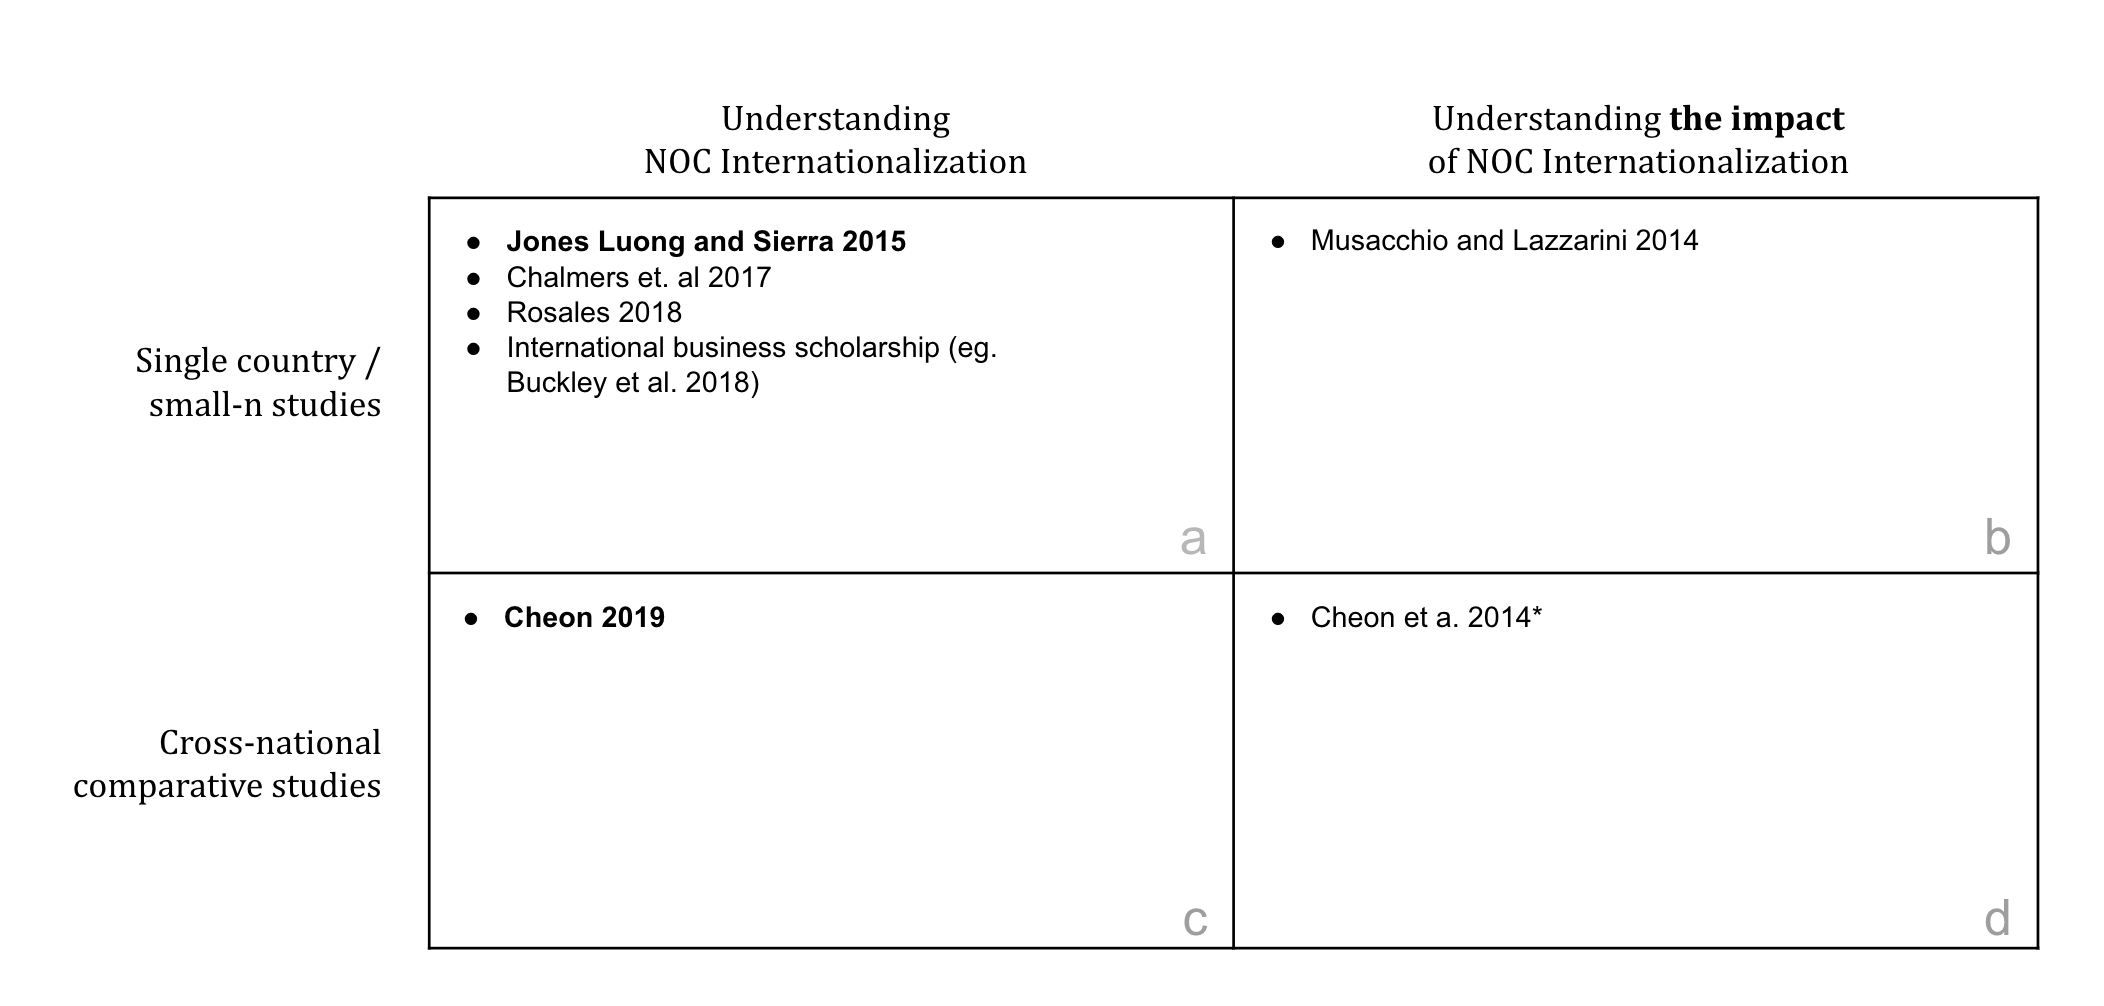
\includegraphics[width=1\linewidth]{fig/typology} 

}

\caption{A typology of the current research on NOC internationalization}\label{fig:typology}
\end{figure}

In subsequent sections I introduce and then explore a new dataset, one that leverages corporate hierarchy data captured in financial databases to develop a rigorous view into the structure of the international hydrocarbon market, including but not limited to NOCs. I then utilize this dataset to investigate a set of questions that build our foundational knowledge of NOC internationalization. As such, the goal of this paper is to contribute to the lower left quadrant in the schematic above (c). Subsequent chapters in this research project contribute to both the upper and lower right of the schematic above (b and d).

\hypertarget{approach01}{%
\section{Empirical Approach: NOC Subsidiary Networks}\label{approach01}}

I gain leverage over NOC internationalization by examining the subsidiary network of each firm and identifying both domestic and international investments and/or operating units. In this dataset the unit of observation is the subsidiary firm. These data are a substantial improvement over previous datasets used in the literature, which in general focus on transactions (mergers \& acquisitions as well as asset purchases) as the unit of analysis. A more direct discussion of these data compared to alternatives is provided in the following subsection. Below I introduce the data source, discuss the data collection process, describe some features of the dataset, and identify the advantages of these data over alternatives.

The base source for all firm level data is Standard \& Poor's \emph{Capital IQ}, a financial services database which provides company profile information about several hundred thousand businesses worldwide. I extracted `corporate tree' information for all NOCs identified above using Capital IQ's report-builder function.\footnote{S\&P Capital IQ. (2017). \emph{Various Company Profiles}. Retrieved April 15-18, 2017, from S\&P Capital IQ database.} A firm's corporate tree identifies all direct subsidiaries, wholly or partially owned. I collected corporate tree data for all 88 parent NOCs identified, producing a dataset of 7,005 observations (where each row is a subsidiary of a specific NOC). Because the headquarters location is coded for both parent and subsidiary, differentiating between domestic and international subsidiaries is straightforward. In addition to identifying the parent and the subsidiary business names, the corporate tree data also indicates whether the subsidiary is an investment or an operating unit, and whether or not the parent has a majority or minority stake in the subsidiary.

I repeated this process to build a dataset of comparable non-state owned energy firms (for simplicity, referred to as international oil companies (IOCs) for the remainder of this document).\footnote{IOCs is technically a misnomer, as at least a few of the firms included in the analysis only operate domestically.} Whereas the NOCs identified represent the universe of NOCs, the potential pool of eligible IOCs is much larger. To simplify the case selection process, I use the FTSE Global Oil \& Gas Index, comprised of major energy firms world wide. After removing several NOCs included in the index I am left with a set of 120 firms.

The combined dataset has a total of 24,724 subsidiaries distributed across 190 parents. Variables coded at the firm level include parent name, subsidiary name, subsidiary type, ownership stake, parent country, subsidiary country, parent founding year, parent employee count. Because both parent and subsidiary locations are coded, the resulting dataset is a rich set of bilateral links that can be easily mapped to state-level features of both the parent and subsidiary (polity scores, GDP/capita, etc.). A reproducible workflow for transforming these data following the initial `report-builder' extract can be found in Appendix \ref{appa}.

A key benefit of the Capital IQ corporate tree data is that the heavy lifting of collecting data has already been done, and has been performed using a range of sources including but not limited to corporate securities filings, annual reports, press releases, and news reports. This range of information provides a broader scope than a single researcher might be able to secure. One important limitation of these data is that they are cross-sectional rather than time-series. While I have information on the founding year for most parents, I have not collected that data for subsidiaries. As such, the data provide a static view of the current state of each corporate tree.

How does this dataset of NOC subsidiaries compare to other efforts to gain leverage over NOC internationalization? As discussed in the previous section, empirical efforts to capture and analyze NOC internationalization have been limited, but a few studies are worth discussing in detail.

Jones Luong and Sierra (\protect\hyperlink{ref-jones_luong_domestic_2015}{2015}) investigate reasons for NOC internationalization head on through a small-n comparative case approach focusing in particular on Latin American NOCs. Their response variable is a factor capturing each firm's degree of internationalization, coded as Low, Medium, or High. This variable is based on three components: the \emph{scope of a firm's foreign operations}, the \emph{degree of foreign investment}, and the \emph{profitability of those investments}:

\begin{itemize}
\tightlist
\item
  \emph{Scope of foreign operations}: operationalized as the number of regions an NOC operates in and the number of activities the NOC is involved in overseas (activities being things like exploration, production, refining, marketing, and distribution). The authors code this based on NOC annual reports, 2000--2010.
\item
  \emph{Degree of foreign investment}: operationalized as the ratio of foreign assets to total assets. This ratio is based on UNCTAD Reports on Transnational Corporations, as well as NOC annual reports.
\item
  \emph{Profitability of foreign investments}: operationalized as foreign revenue as a percentage of total revenue. This is coded based on Security \& Exchange Commission Form 20F releases.
\end{itemize}

This measure, while exceptionally useful, has some important limitations. First, the approach relies on a significant amount of hand coding of primary source documents, annual reports in particular. In addition to being arduous work, data availability is a concern: many NOCs do not publicly release an annual report. Second, the factor and index nature of the measure obscure important variation in the data. By summarizing the measure into three levels, Jones luong and Sierra are losing valuable granular information about how internationalization varies from firm to firm. And by combining several elements into an index, it becomes difficult to identify how the components relate (or whether certain components are driving the overall index more than others).

Cheon (\protect\hyperlink{ref-cheon_developing_2019}{2019}) tackles a similar question with different data. He takes a quantitative approach to understanding variation in internationalization across the population of NOCs. He tests a number of hypotheses on mergers \& acquisitions data accessed through GlobalData's E-Tracks M\&A database. The unit of analysis is a specific transaction, which is then coded for relevant features (including date, transacting parties, type of asset, etc.). E-Tracks data have a number of attractive features. Because transactions are dated, the data give a longitudinal view of investment activity. Additionally, the dataset is quite large and a substantial amount of detail is captured for each transaction.

However, these data have some shortcomings worth considering. First, transaction values are only available for a subset of observations, leaving the researcher with a choice of either using the subset with dollar values indicated or replace an interest in transaction value with volume (operationalized as a count of transactions). This approach is not able to differentiate between small and large transactions. Second, firm identifiers are not consistently coded in the data; nor is it immediately apparent whether the transacting party is a parent firm or a subsidiary of another entity. Both of these factors make it difficult to accurately link specific transactions back to the right corporate entity. Third, investments often involve a number of transacting parties, of which only one might be an NOC; parsing out these multi-party transactions is difficult, involves substantial manual effort, and raises many opportunities for coder error. Fourth, the sources of these data are industry reports and press releases: this raises the concern that some firms may be systematically under-represented in the data. A final consideration is that the researchers have not made this dataset publicly available at this point in time.

\hypertarget{analysis01}{%
\section{Analysis: Variation in NOC Internationalization}\label{analysis01}}

This section proceeds down three primary paths. First, we describe basic features of how internationalization varies across NOCs (and IOCs). While methodologically unsophisticated, our objective is important: NOC internationalization has received relatively little empirical attention to date, and we lack satisfactory answers to a number of basic questions. Descriptive analysis of this sort is an essential baseline for more sophisticated inferential/theoretical work. Section \ref{descriptivestats01} addresses the following questions:

\begin{itemize}
\tightlist
\item
  How many NOCs have at least one international subsidiary?
\item
  How is internationalization distributed across firms?
\item
  Which industries and asset structures (ie. joint ventures, minority-owned, investments or operating units) are most common? How do NOCs vary in terms of the structure of their international footprint?
\end{itemize}

In section \ref{network01}, we analyze the relationships between firms and subsidiaries to shed light on how NOC internationalization varies as a network. \textbf{Come back to this and build it out.}

\begin{itemize}
\tightlist
\item
  How do NOC subsidiary networks vary in terms of the number of distinct nodes or the geographical dispersion of subsidiaries?
\item
  Which states are at the core of the global network of NOC internationalization, and which are at the periphery?
\end{itemize}

In \ref{iocnoc01}, we investigate whether the pattern of NOC internationalization differs measurably from how IOCs are structured as multinational firms. In particular, we examine the political affinity between home and host states. Are NOCs more likely to invest in states that are more politically alike? \textbf{Come back to this and build it out.}

\hypertarget{descriptivestats01}{%
\subsection{How does NOC internationalization vary?}\label{descriptivestats01}}

Of the 87 NOCs identified, we were able to collect corporate hierarchy data on 77 distinct firms across 64 countries. 60 of these firms have at least one international subsidiary. NOCs have a median number of 18 international subsidiaries, compared to a median of 27 in the sample of IOCs captured. Summary statistics can me found in Table \ref{tab:sumstats}.

Of the 87 NOCs identified, we were able to collect corporate hierarchy data on 77 distinct firms across 64 countries. 60 of these firms have at least one international subsidiary. NOCs have a median number of 18 international subsidiaries, compared to a median of 27 in the sample of IOCs captured. Summary statistics can me found in Table \ref{tab:sumstats}.

\begin{table}

\caption{\label{tab:sumstats}Summary Statistics: NOC Subsidiaries}
\centering
\begin{tabular}[t]{lrrrrrr}
\toprule
\textbf{Type} & \textbf{Mean} & \textbf{Median} & \textbf{Std. Dev} & \textbf{Min} & \textbf{Max} & \textbf{Total}\\
\midrule
domestic & 58.9 & 18.5 & 106.6 & 1 & 554 & 4125\\
international & 47.5 & 22.5 & 58.2 & 1 & 305 & 2754\\
\bottomrule
\end{tabular}
\end{table}

Figure \ref{fig:distributions} below visualizes the distribution of NOCs and IOCs by the number of international subsidiaries they have. The untransformed distribution is strongly right-skewed, and so the axis has been log10 transformed to better visualize the variation in the data. An alternative view utilizing boxplots can be found in the appendix (Figure \ref{fig:boxplot1}).

\begin{figure}

{\centering 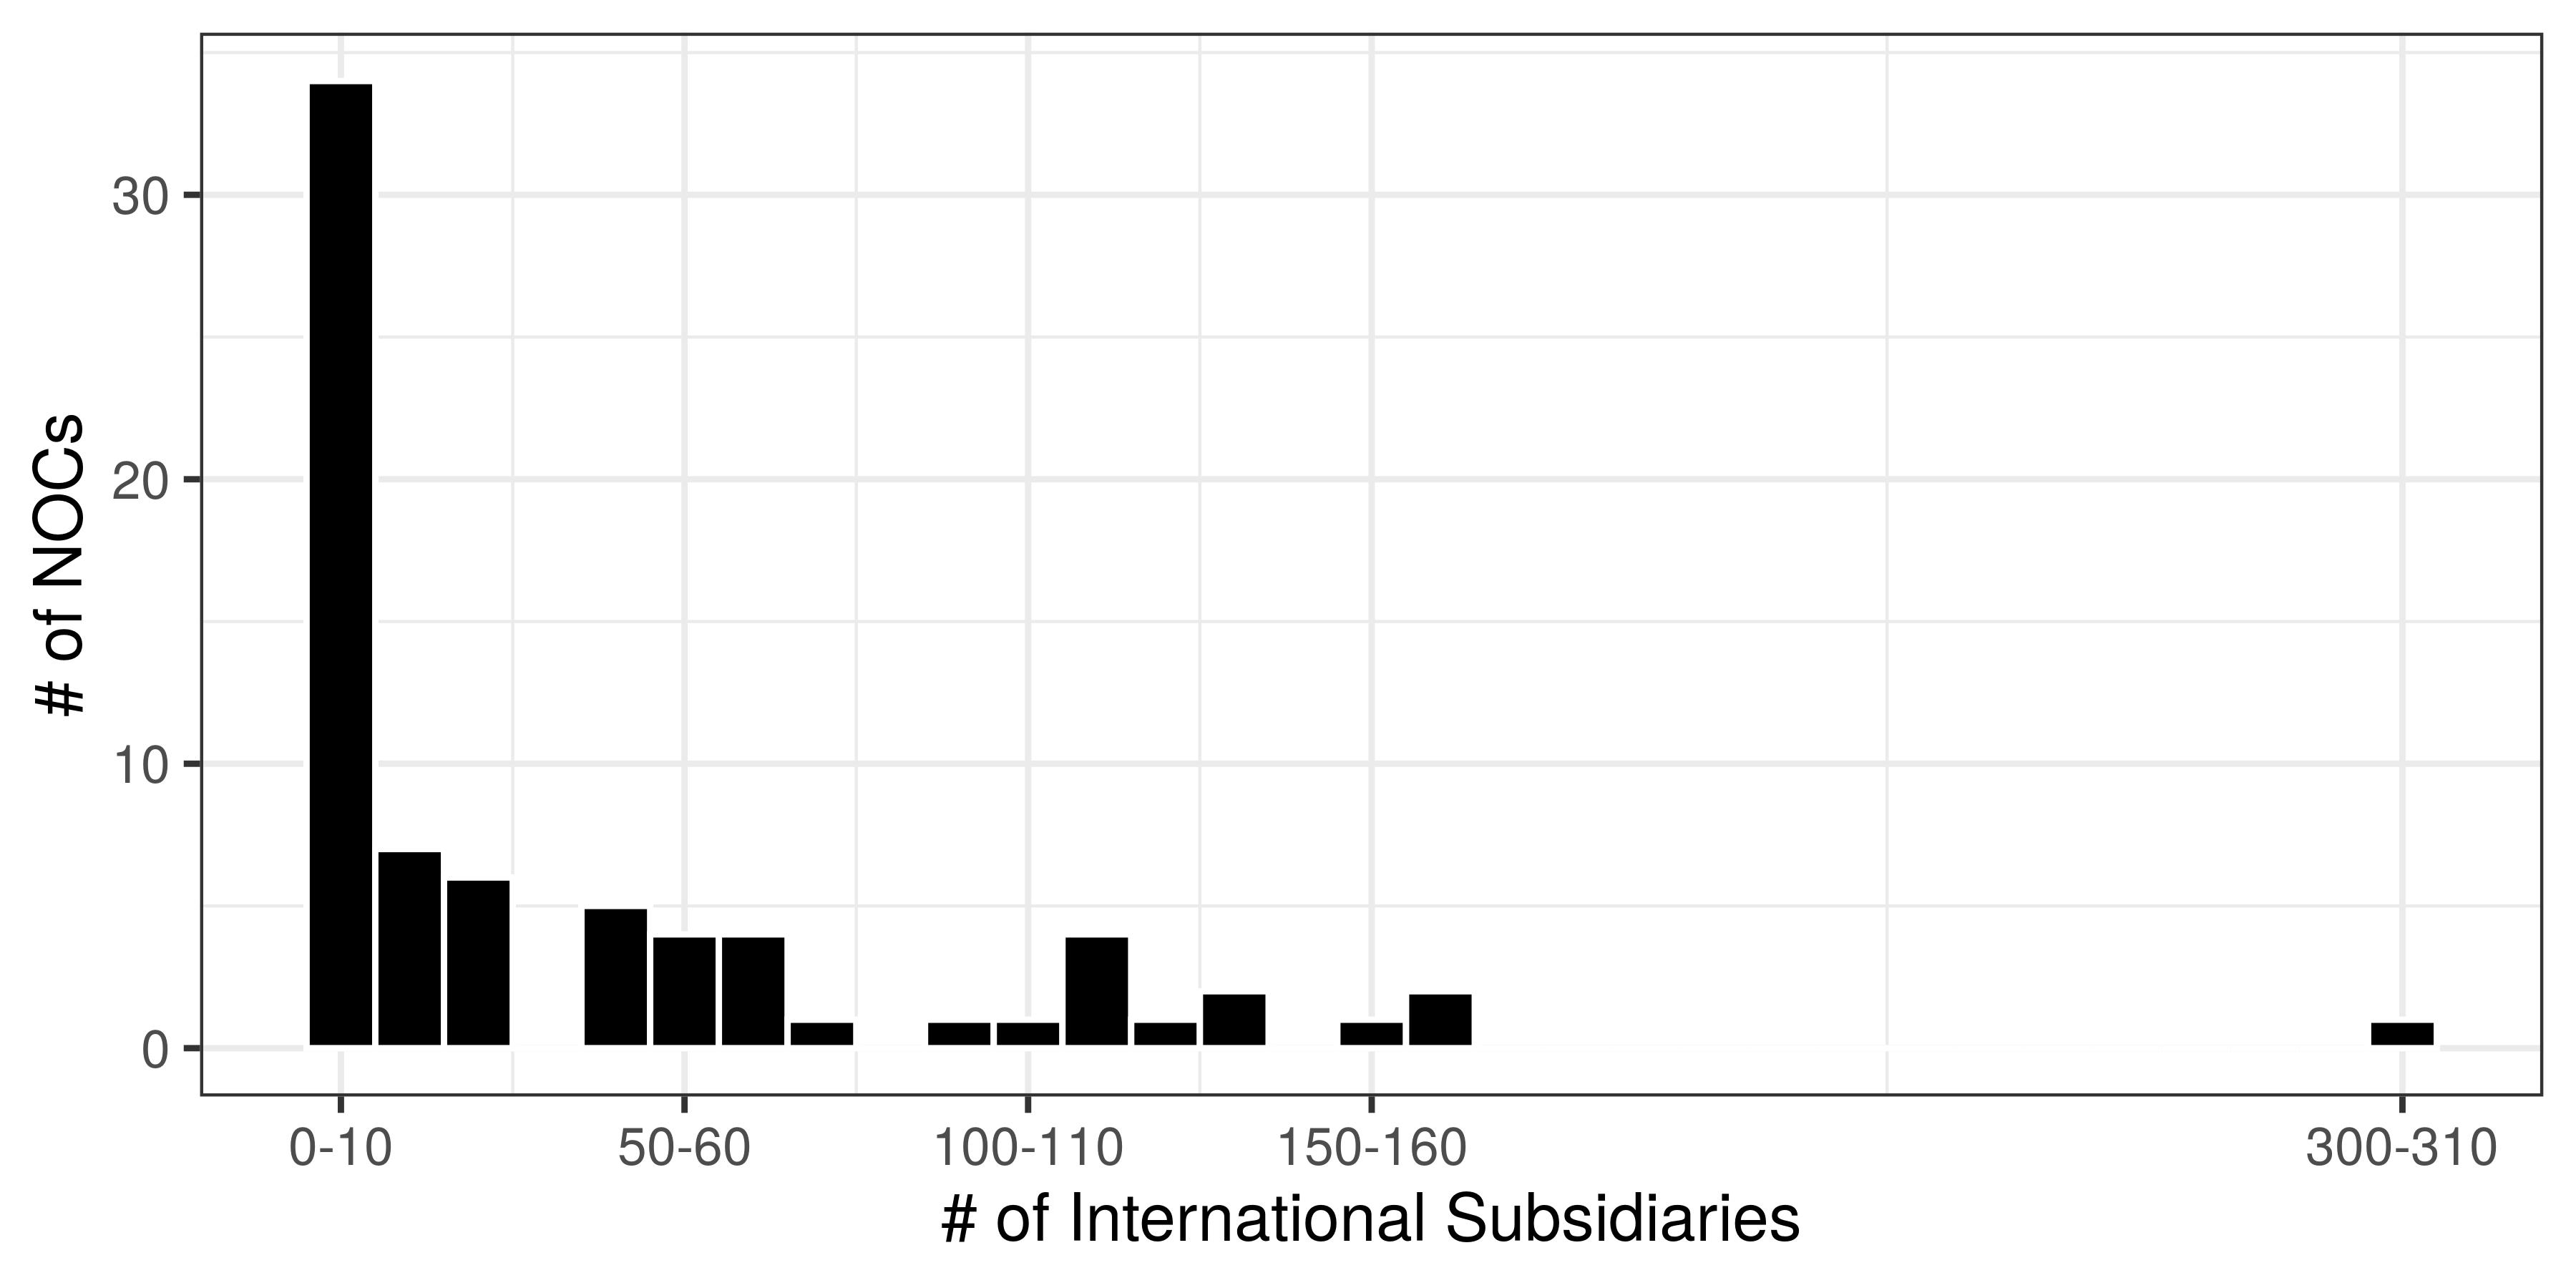
\includegraphics[width=0.8\linewidth]{finalfig/distributions-1} 

}

\caption{Distribution of International Subsidiaries}\label{fig:distributions}
\end{figure}

European NOCs generally have the most international subsidiaries. Eni has 305, spread across 54 different host states. Equinor (formerly Statoil - Norway, 161 international subsidiaries), MOL (Hungary, 143), Gazprom (Russia, 130), and OOC (Oman, 125) round out the top five. Of these, only Gazprom and OOC are majority state-owned.\footnote{In each of the other firms, the state maintains a substantial minority stake in the firm and is the largest stakeholder.} A list of the top 20 NOCs by international subsidiaries can be found in \ref{tab:toptbl}.

\begin{table}

\caption{\label{tab:toptbl}Internationalized NOCs}
\centering
\begin{tabular}[t]{llrr}
\toprule
\multicolumn{2}{c}{ } & \multicolumn{2}{c}{Subsidiary Type} \\
\cmidrule(l{3pt}r{3pt}){3-4}
\textbf{Firm} & \textbf{State} & \textbf{Domestic} & \textbf{International}\\
\midrule
\textbf{Eni} & \textbf{Italy} & \textbf{93} & \textbf{305}\\
Statoil & Norway & 128 & 161\\
Gazprom & Russia & 484 & 158\\
MOL & Hungary & 73 & 149\\
OMV & Austria & 36 & 127\\
\addlinespace
OOC & Oman & 19 & 127\\
Rosneft & Russia & 554 & 119\\
SOCAR & Azerbaijan & 19 & 114\\
CNOOC & China & 328 & 112\\
Petronas & Malaysia (1966-) & 190 & 111\\
\addlinespace
DONG & Denmark & 59 & 107\\
Sonangol & Angola & 36 & 105\\
CNPC & China & 341 & 90\\
KPC & Kuwait & 13 & 74\\
KNOC & Korea, South & 7 & 64\\
\addlinespace
PTT & Thailand & 122 & 62\\
Saudi Aramco & Saudi Arabia & 23 & 61\\
Petrobras & Brazil & 122 & 59\\
ONGC & India & 46 & 55\\
Sonatrach & Algeria & 22 & 55\\
\bottomrule
\end{tabular}
\end{table}

At the other end of the distribution, there are at least 17 NOCs that do not have any recorded international subsidiaries in the dataset, and another 5 that have only one. CUPET, Cuba's NOC, has one identified international subsidiary: a minority investment in Angola's Cabinda Onshore South Block oil concession. Uzbekneftegaz, Uzbekistan's NOC, has two: gas utility subsidiaries in China and South Korea.

There are 2,638 international subsidiaries spread across the 60 NOCs that have at least one international subsidiary. 66\% of these subsidiaries are majority owned by the NOC parent (24\% are minority-owned, and 10\% of subsidiaries do not have ownership amount available). They are spread across a number of different industries, the most common being exploration \& production, refining \& marketing, and storage \& transportation, though we are lacking data on a significant percentage of subsidiaries.

\hypertarget{network01}{%
\subsection{What does the international NOC network look like?}\label{network01}}

The relationship between an investing firm and the state its subsidiary is registered in should be treated with significant care. An Eni example illustrates this effectively. Eni has 44 subsidiaries in the United Kingdom; one of these is Burren Energy PLC. Burren was a British firm prior to its acquisition by Eni, but at the time of acquisition it had active or former concerns in Yemen, Oman, Egypt, Turkmenistan, India, and Congo. When a subsidiary is itself a multinational corporation, this can have substantial confounding effects on our ability to appropriately assess the kind of internationalization pursued by the parent firm.\footnote{Another challenge is that some host states --- the United Kindgom and the Netherlands chief among them --- have sub-jurisdictions that are magnets for offshore investments or tax avoidance. These include Jersey, and the Cayman Islands, for example. NOCs (and IOCs) have many subsidiaries in these types of jurisdictions, indicating that tax havens play an important role in the structure of the global market for hydrocarbons.} With these caveats in mind, however,it is worth understanding how NOC networks vary.

In general, firms with more international subsidiaries have them in a broader range of locations (Figure \ref{fig:scatter01}). Equinor (formerly Statoil, the Norwegian NOC) has 161 international subsidiaries spread across 39 different countries, with a median of 2 subsidiaries per country. Petronas, the Malaysian NOC, has fewer international subsidiaries (111) but spread across a larger number of countries (46).

Figure \ref{fig:scatter01}) is a highly informative representation of how internationalization varies across NOCs. There are only a few firms that have both a large and broad-based international presence: Eni is the runaway outlier in both respects, but this group also include Equinor (Statoil), Petronas, Gazprom, Rosneft, the Oman Oil Company (OOC), OMV, MOL, SOCAR, Sonangol, and CNPC. Many of these are NOCs with strong commercial institutional characteristics (a minority of shares floated on the stock market, for instance). DONG and Petronas are both outliers of sorts. DONG has a large number of international subsidiaries but more than half of them are in one subsidiary state, Germany. Petronas has fewer international subsidiaries than many of these other internationalized NOCs, but has them spread across more subsidiary states than any other firm save Eni.

\begin{figure}

{\centering 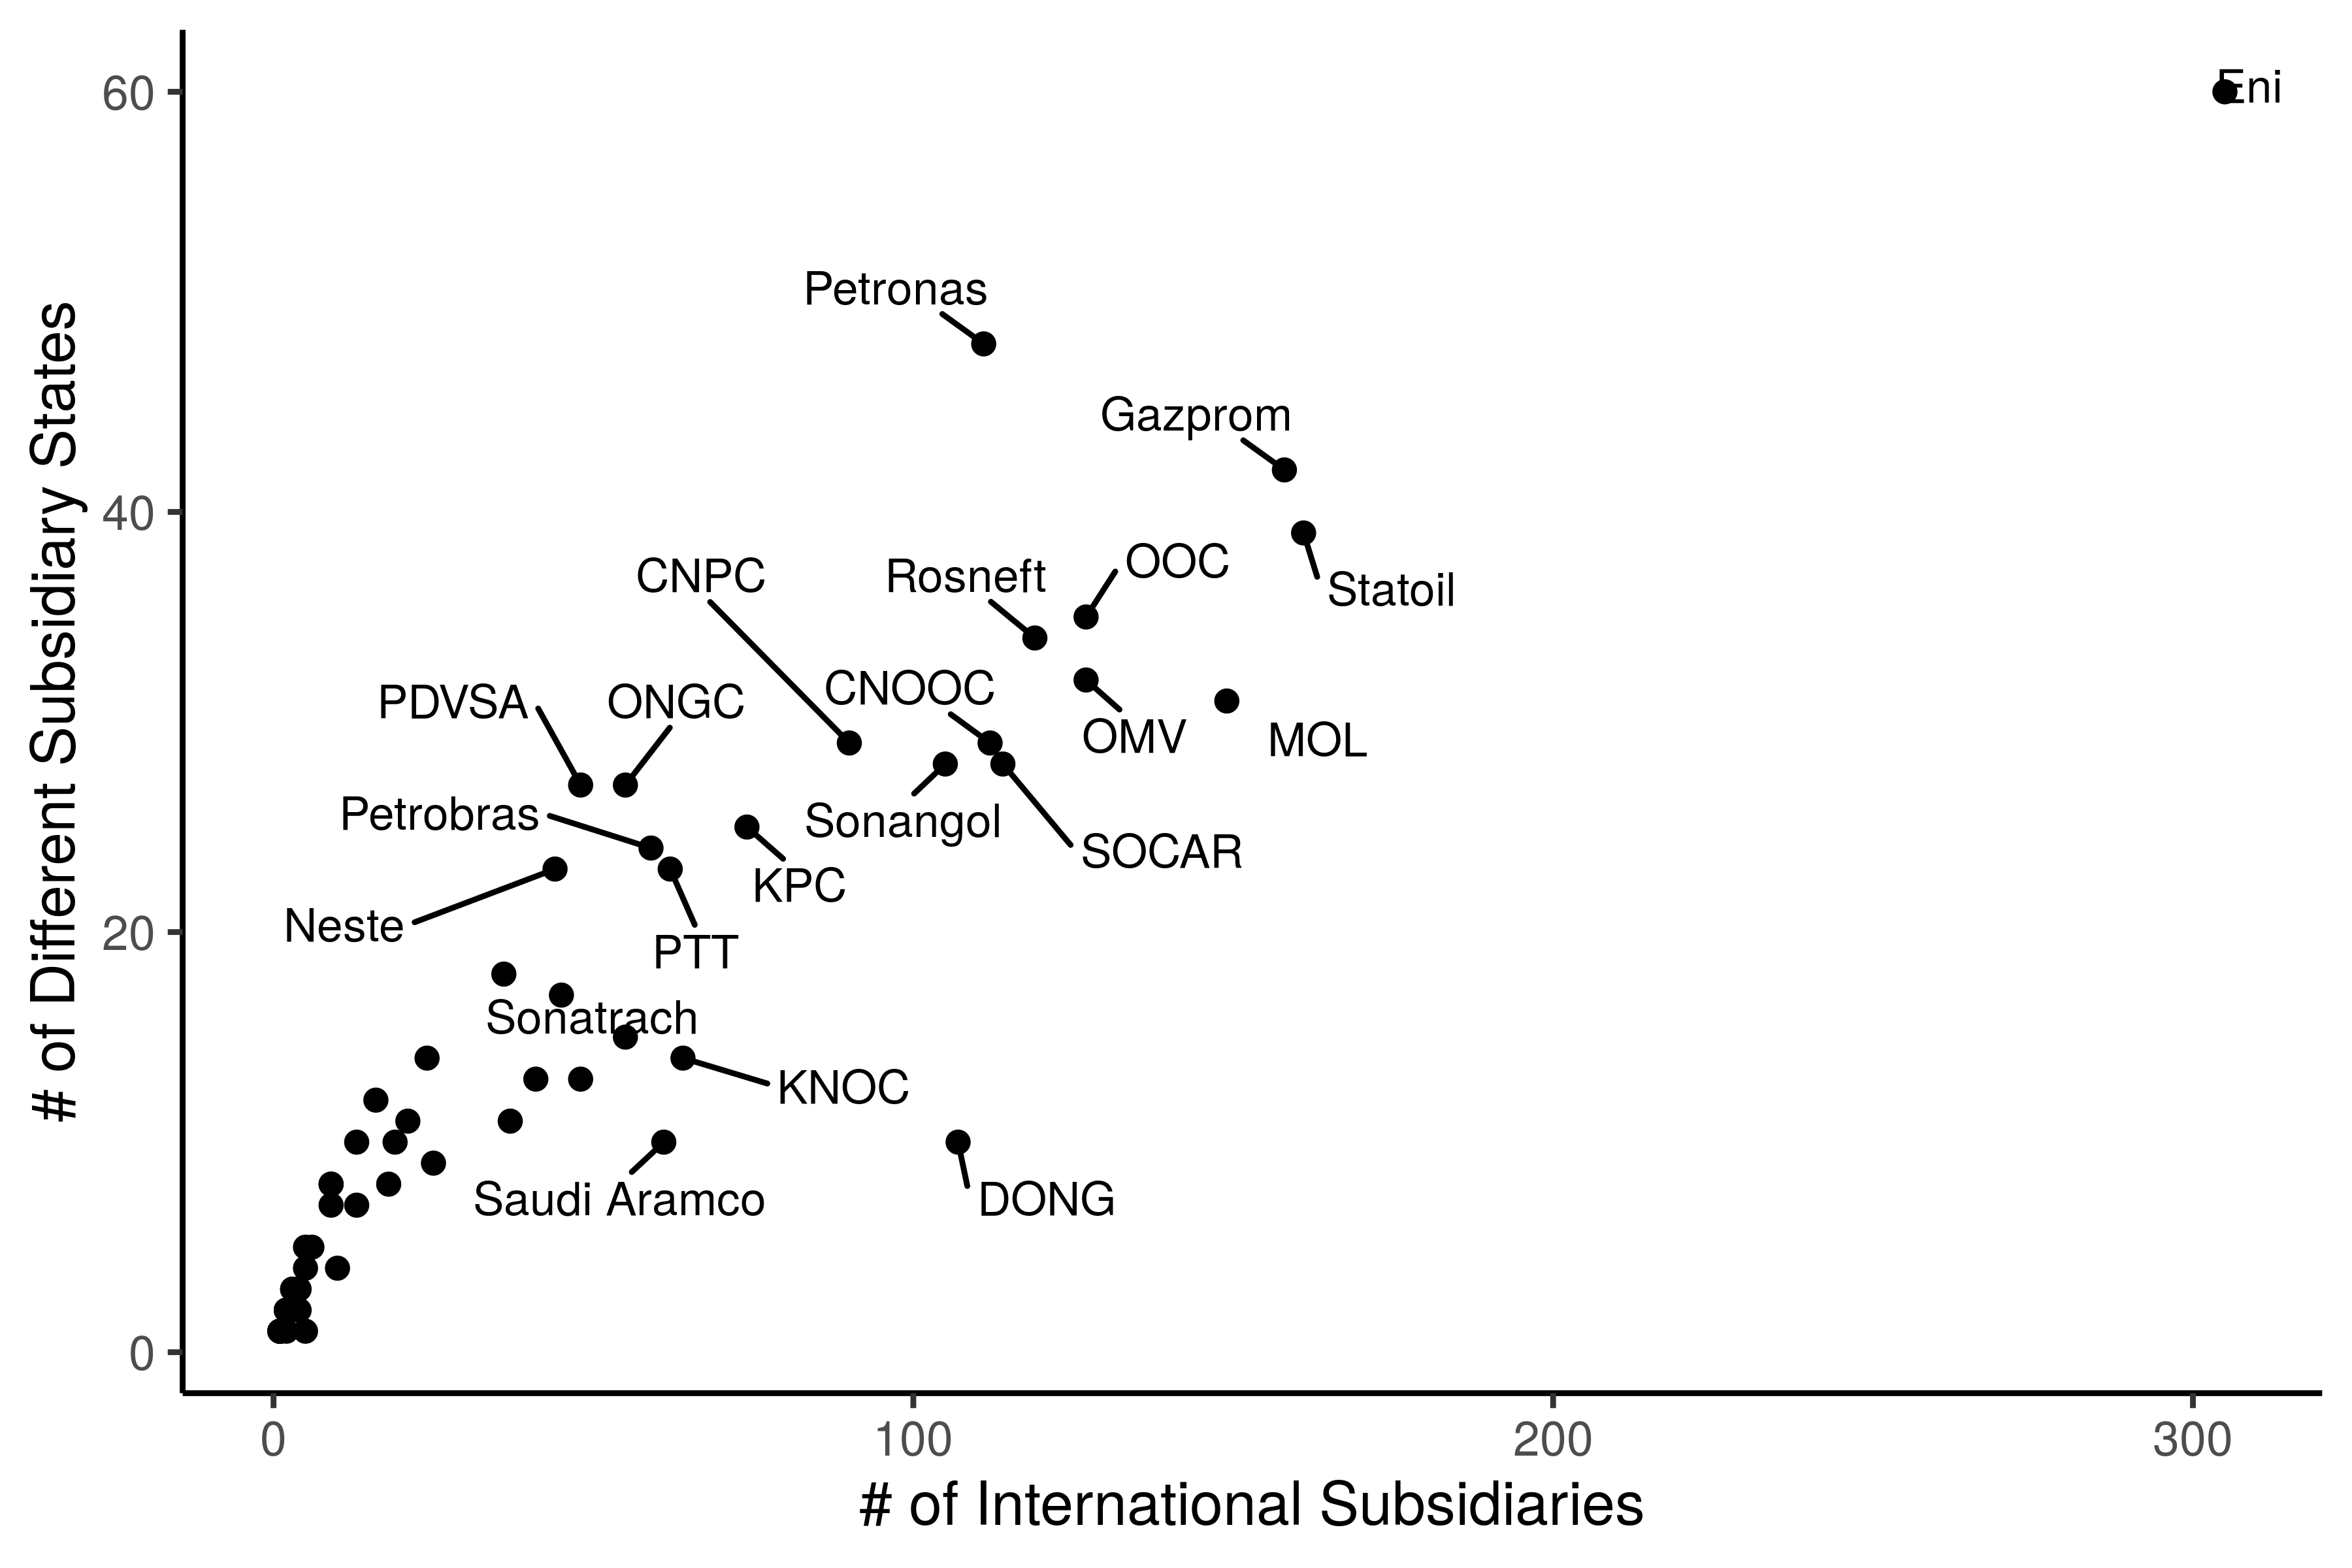
\includegraphics[width=0.8\linewidth]{finalfig/scatter01-1} 

}

\caption{NOC Internationalization: Total number of International Subsidiaries (x) correlates strongly with breadth of the international subsidiary network (y). Points sized by median number of subsidiaries per location.}\label{fig:scatter01}
\end{figure}

One of the best ways to visualize this variation is using maps. Figure \ref{fig:t6map} visualizes the subsidiary network for the NOCs with the most international subsidiaries by drawing a line between the home state and the subsidiary state (endpoints for both are the state capital, as subsidiary specific headquarters data is difficult to geocode with reliability).

\begin{center}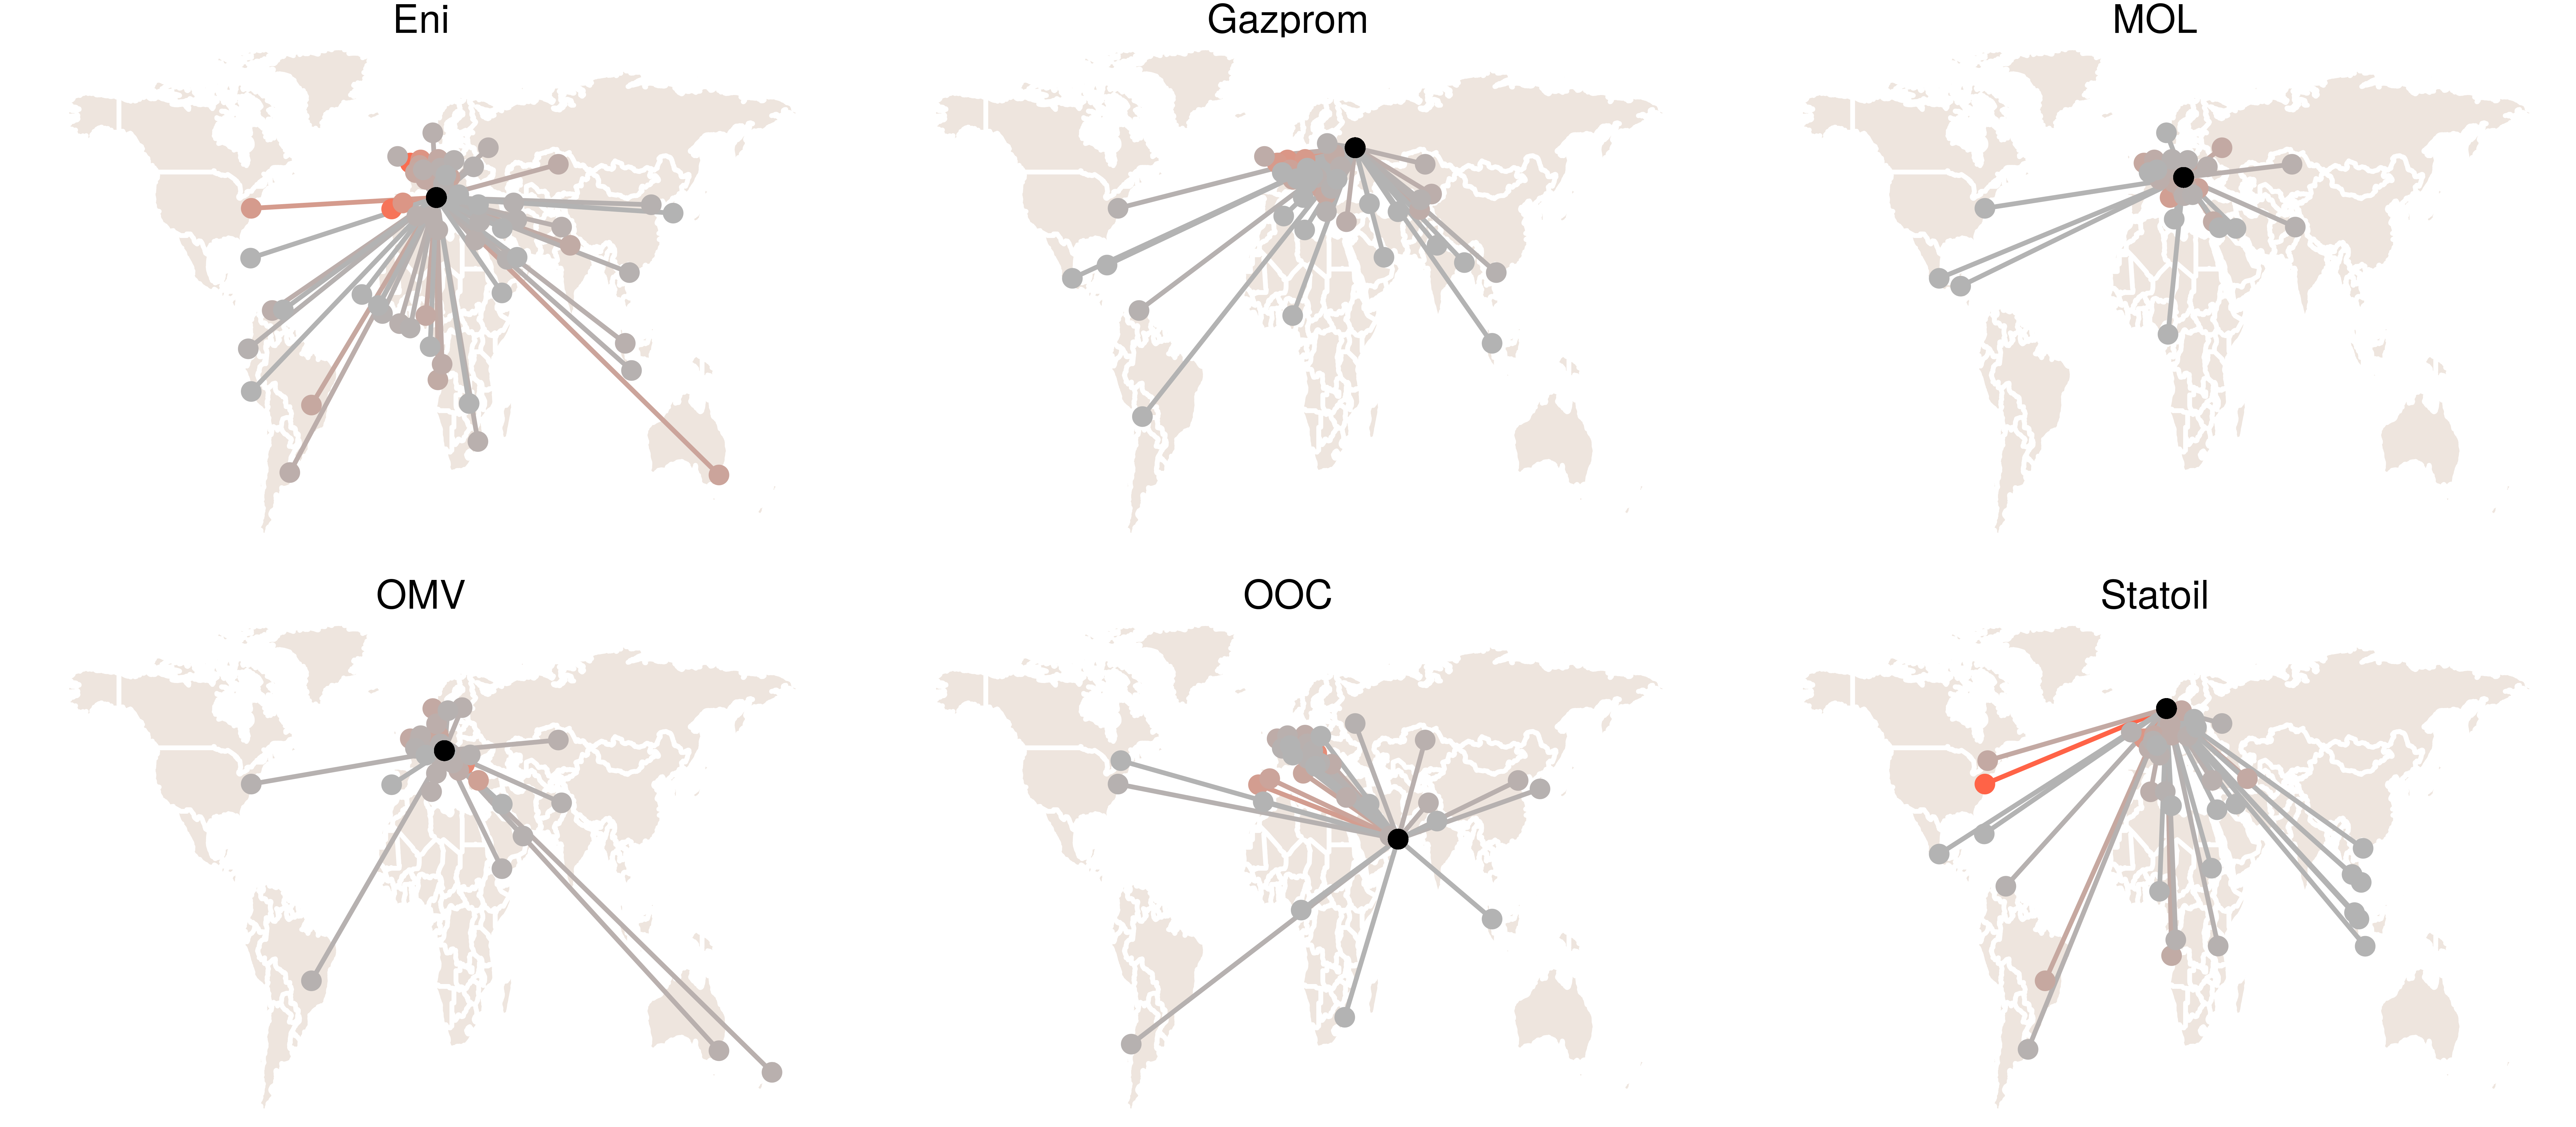
\includegraphics{finalfig/t6map-1} \end{center}

These visuals reveal several interesting patterns that might not otherwise be apparent without showing the spatial data on a map. Statoil and Eni have the broadest (and largest) international networks, but they differ substantially from one another: Eni is more heavily invested in Africa and East Asia than Statoil. Gazprom, MOL and OMV concentrate their investments within a relatively narrow geographical scope: none have developed a presence in East Asia, and OMV is the only one with subsidiaries in South America.

An alternative way to think about internationalization isn't the absolute degree of internationalization achieved by a given firm, but rather whether that firm over- (or under-) indexes on internationalization given what we know about it. Which firms ``punch above their weight'' from an internationalization persepective? Using the subsidiary networks dataset, one way to do this might be to index international subsidiaries to domestic subsidiaries. In general larger, more capable or more well-endowed firms should have both a substantial international presence and a network of subsidiaries domestically to handle (the correlation between the two is moderately positive, at 0.47 {[}0.27, 0.63{]}).

The table above lists the firms that strongly over-index in internationalization: they have at least three times as many international subsidiaries as domestic ones. This approach brings some new firms to prominence. KNOC, South Korea's firm, was not previously identified as a highly internationalized firm, but its international network relative to the scale of its domestic operations is dramatic. Finland and Saudi Arabia are similar. There are also, however, a number of firms that should be classed as highly internationalized by both approaches, absolute size of the international network and relative to the domestic network: OOC, SOCAR, KPC, Sonangol, OMV, ENI.

\hypertarget{iocnoc01}{%
\subsection{Are there political differences in how NOCs invest?}\label{iocnoc01}}

Is NOC internationalization measurably different from the international networks developed by non-state owned international oil companies? As discussed above, there is a clear difference in degree or size: the top IOCs generally have much larger and more extensive international networks than NOCs. Does that difference persist when we consider the kind of network NOCs develop? This section considers whether NOC and IOC investment networks different in terms of the political affinity between home and host state. Political affinity in the subsidiary network is one of the most interesting potential points of departure between IOCs and NOCs. On one hand, if there is no measurable difference in the networks, then our case for focusing research into NOCs as a distinct set of firms is undermined.

I operationalize this question in the following way. First, I re-frame it in terms of a testable hypothesis. If NOCs do invest politically, then there will likely be a systematic difference between how they invest and how peer IOCs invest. This difference will relate to the degree to which the pattern of investments reflects state preferences. If NOCs invest politically, the pattern of their investments should reflect the political preferences of the state such that NOC patterns are systematically different from IOC investment patterns.

To measure that difference, I consider the state ideal point proximity between parent and subsidiary firms for all international parent-subsidiary relationships for both NOCs and IOCs. High proximity is reflected in a small absolute difference between ideal points: parent and subsidiary states are quite similar in terms of their political preferences via-a-vis the US led international order. Alternatively, low proximity (reflected in a large absolute difference) indicates that the two states have very different perspectives and preferences.

The hypothesis I investigate is that NOCs are indeed a different type of firm, one that behaves differently when it comes to their international expansion. I hypothesize that this underlying difference will be expressed in the pattern of investments they make and subsidiaries they establish, particularly in terms of the relative political characteristics of the relationship.

I investigate this by regressing the absolute difference between parent and subsidiary stage ideal points on a dichotomous term indicating whether or not the parent is an NOC, the ideal point of the parent state, and a vector of other covariates to control for observable differences between NOCs and IOCs. The coefficient on the NOC/IOC dichotomous term captures the difference between groups.

The results of this analysis allow me to reject the null hypothesis that there is no systematic difference between NOCs and IOCs in terms of the political proximity of their subsidiaries. Controlling for observable differences, NOC subsidiaries are likely to be between .2 and .3 ideal points closer to their parent than IOC subsidiaries. This result is consistent across several specifications, including models with both region and country fixed effects.

The outcome variable I employ is the absolute difference between parent and subsidiary state ideal points based on United Nations (UN) General Assembly votes. These data are a combination of Capital IQ subsidiary data and UN voting ideal point data (Bailey, Strezhnev, and Voeten \protect\hyperlink{ref-bailey_estimating_2017}{2017}). As discussed earlier, subsidiaries are coded both for their headquarter location and the headquarter location for their parent firm. My subsidiary dataset is comprised of 10,471 subsidiaries; 2,746 of these are subsidiaries of NOCs. All of these are international subsidiaries: the headquarters of the parent and the subsidiary are in different states.

State ideal points capture ``state preference over foreign policy\ldots{} on a single dimension that reflects state positions toward the US-led liberal order'' (Bailey, Strezhnev, and Voeten \protect\hyperlink{ref-bailey_estimating_2017}{2017}, 430).\footnote{I refrain from developing a more detailed discussion of these data here, given the purpose of the document and the reader's intimate familiarity with them.} Ideal points don't directly reveal or capture how similar states are in terms of their foreign policy preferences, but rather how comparable they are on a common scale, in terms of a common position vis-a-via the US-led international order. I refer to this comparability as political affinity.

I merge in state ideal points for both parent and subsidiary; the absolute difference between these values provides a subsidiary-level measure of the ideal point proximity --- and thus, the political affinity --- between the subsidiary state and the parent state. Absolute differences range from 0 to 4.4, with a mean of 1.3 and a standard deviation of 0.9. The treatment of interest is a dichotomous indicator that takes 0 if the parent is an IOC and 1 if the parent is a NOC.

In order to operationalize H1, I regress the absolute difference on a dichotomous indicator for whether or not the parent is an NOC and a vector of covariates that account for observable differences between NOCs and IOCs. The term on the NOC/IOC indicator can be interpreted as the impact of being an NOC relative to an IOC on absolute differences, conditional on covariates.

Prior to conducting regression analysis, I probed the plausibility of this difference visually and using a difference in means test. Visualization of the distribution of ideal point absolute differences for both NOCs and IOCs offer some preliminary support for contention that there is a difference between groups. While both distributions are left-censored with a long right tail, NOCs display more relative density at the lower end of the absolute difference range than IOCS. A difference-in-means t-test confirms that there is s statistically significant difference between mean absolute difference values for NOCs when compared to IOCs. In general, these results suggest that NOCs tend to set up subsidiaries such that the aggregate absolute difference between parent and subsidiary ideal points is less than IOCs. In other words, political affinity between parent and subsidiaries is higher, on average, in the NOC data than in the IOC data.

I control for parent state ideal point to capture the intuition that absolute difference might be primarily driven by the relative difference in NOC and IOC parent ideal points. Perhaps parent-subsidiary ideal point absolute difference is purely a function of the fact that NOC parents generally have lower ideal points than IOC parents, as do subsidiaries. The inclusion of this covariate should allay some of these concerns.

I also control for observable differences between IOCs and NOCs related to oil production, oil exports, oil rents as a share of government revenue, gross domestic product, and GDP per capita. All of these are likely to explain some variation in how the outcome varies across NOC/IOC groups. Finally, I control for region as well as country. Regional fixed effects capture any systematic variation at the regional level, and country fixed effects to capture any unexplained state-level variation. Various specifications are summarized in the regression results (Table) below.

\begin{figure}

{\centering 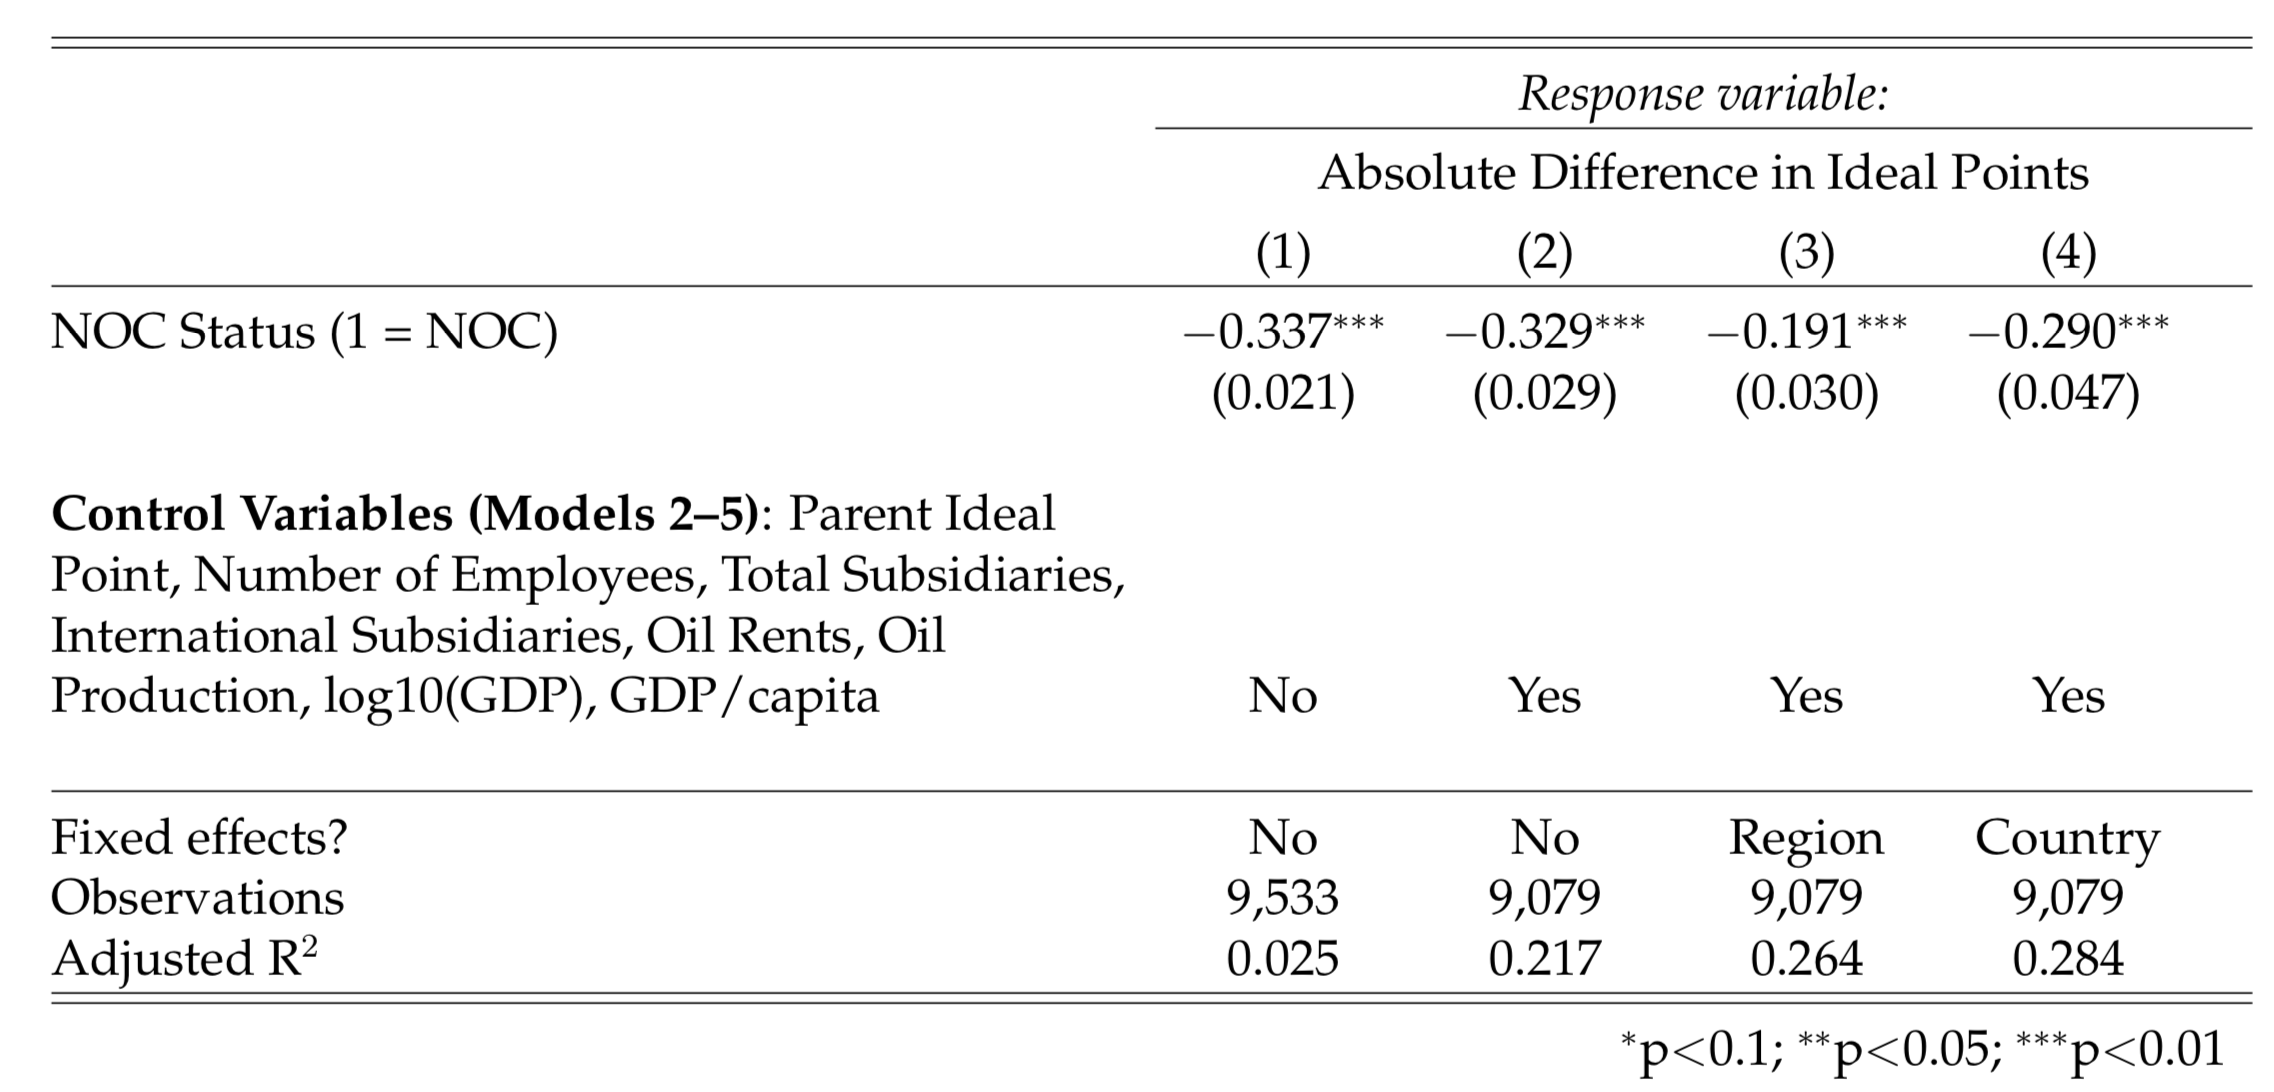
\includegraphics[width=1\linewidth]{fig/reg_results_01} 

}

\caption{Results}\label{fig:regress}
\end{figure}

The regression approach developed here provides a basis to reject the null hypothesis that there is no difference between NOCs and IOCs in terms of subsidiary investment patterns. NOC parent status is associated a substantive and statistically significant reduction in the ideal point absolute difference between parent and subsidiary across all specifications. The sign and strength of this association is consistent across specifications. Depending on model, point estimates for the effect of NOC status range from -.191 to -.337; all estimates are significant at the 99\% level. The coefficient from the most restrictive specification with country fixed effects included is -.29, which is just under 1/3 of the standard deviation for ideal points in the data.

\hypertarget{conclusion01}{%
\section{Discussion}\label{conclusion01}}

\hypertarget{paper2}{%
\chapter{Why do some NOCs go global?}\label{paper2}}

\hypertarget{intro02}{%
\section{Introduction}\label{intro02}}

Nigeria and Angola are the two largest oil producers in Africa, and their NOCs (NNPC and Sonangol, respectively) are two of the most important domestic economic institutions. Both countries have significant levels of international investment into their oil sectors. Both experienced devastating civil conflict until early in the 21st century. Nigeria has a much larger population and economy; Angola performs better, comparatively speaking, on indexes that measure corruption and investment risk.

Despite striking similarities in the area of hydrocarbons in particular, NNPC and Sonangol have strikingly different international footprints (Figure \ref{fig:sonanNNPC}). Sonangol is one of the most global NOCs in the world: it has substantial ties to Portugal (perhaps unsurprising, given the colonial history the two states share) but it also has subsidiaries across Europe and the Americas. It is invested throughout the African continent. NNPC, despite being one of the largest oil firms in terms of production capacity and resource base, an extremely small international presence: offshore financial subsidiaries in the United Kingdom and Panama, and one liquefied natural gas (LNG) subsidiary in Ghana. This difference is a striking example of variation in NOC internationalization. Like Sonangol,some NOCs have developed an extensive international footprint: they have investments and operating units across a wide range of states, up and down the hydrocarbon value chain. Other NOCs (even large, high-production firms like NNPC) haven't developed that footprint to nearly the same extent, or at all. What explains this variation?\footnote{Chapter @ref(\#paper1) investigates this variation in detail.}

\begin{figure}

{\centering 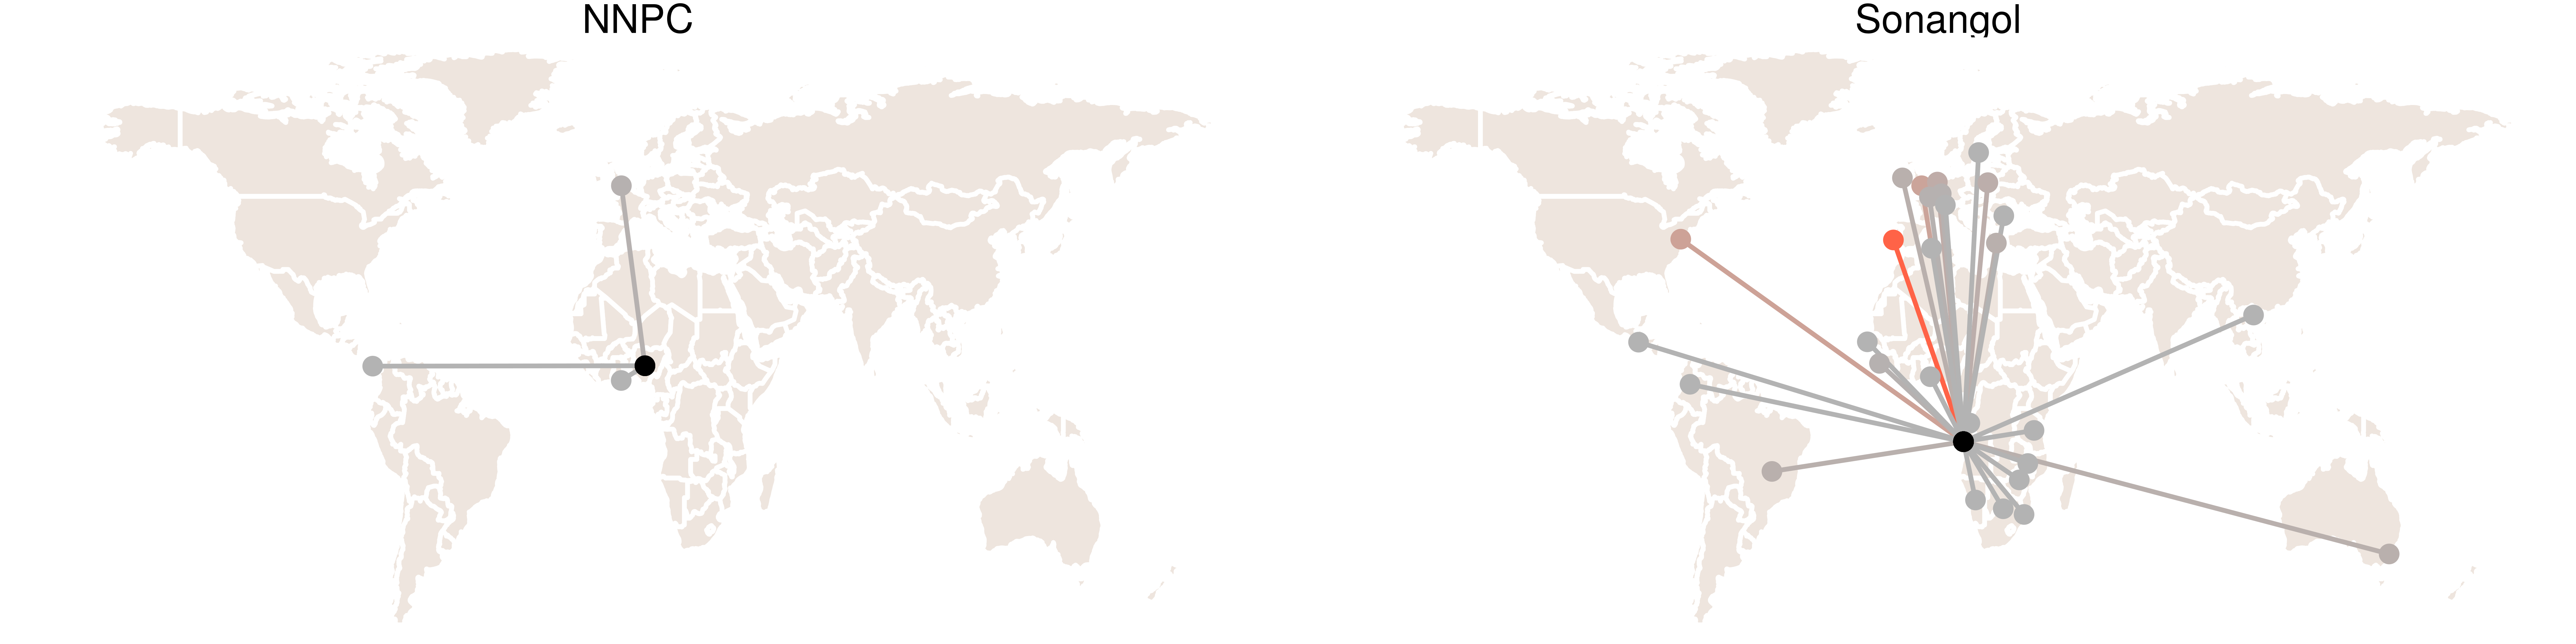
\includegraphics{finalfig/sonanNNPC-1} 

}

\caption{NOC internationalization: comparing Nigeria and Angola}\label{fig:sonanNNPC}
\end{figure}

The bulk of empirical work addressing NOC internationalization is focused on this question. Political economists and international business scholars have offered several different explanations for why some NOCs go global and others stay at home. This focus is unsurprising. NOC internationalization is one of the most important ways resource-rich states interact with and play an active role in the global economy. The conditions or processes that give rise to this phenomenon are at the heart of what state capitalism is in the context of contemporary political economy, and touch on core concerns as to how social and political influences and institutions play a role in shaping economic outcomes like trade networks and hydrocarbon supply flows.

Existing explanations for NOC internationalization are, however, constrained in at least two interrelated ways. First, most studies have been developed in a relatively data-sparse environment. Second, many scholars have pursued within-country or small-n case comparative approaches to theory-building and empirical investigation. These choices have likely been influenced by the lack of good cross-national data on NOC internationalization. Approaching the question through a within-country or small-n comparative lens has advantages, but significant limitations as well. Quantitative studies that focus on single countries side-step the problem of poor cross-national data and leverage rich firm-level data in the context of a specific state (many of these focus on China). While grounded in excellent data and rigorous methodologies, however, these studies necessarily struggle to substantiate generalizable claims that explain variation broadly speaking. Qualitative studies encounter the same tradeoff: they are able to apply detailed and insightful information to the task of elucidating the mechanisms that connect political/social influences to outcomes of interest (NOC internationalization chief among them), but we aren't able to draw strong conclusions about how these mechanisms work across the broad range of NOCs in operation globally.

In this chapter we make two moves to improve this situation. First, we take a graph-based approach to causal inference and theory-building (Pearl \protect\hyperlink{ref-pearl_causality_2000}{2000}). Using directed acyclic graphs (DAG) we formalize a diverse set of expectations about the factors that should influence NOC internationalization into a graphical causal model. This approach has two key benefits: it forces us to explicitly state our theoreical propositions and build them up into a coherent theory, and it allows us to assess whether our model is identified. Second, we evaluate our model's propositions empirically using a novel data source, NOC subsidiary networks (introduced in Chapter 1).

We argue that NOC internationalization is the product of a set of causal processes that range from the immediate, including the decision-time preferences of the stakeholders tasked with deciding on each opportunity for further internationalization, to historical, such as the ways by which authoritarian leadership dynamics are translated into governance structures and tools of institutional oversight. We find that \textbf{Insert specific empirical findings here}

The chapter proceeds as follows. In the following section (\ref{motiv02}) we clearly outline existing explanations for NOC internationalization, focusing on establishing testable hypotheses and a catologue of causal mechanisms proposed across the literature. In section \ref{approach02} we outline our approach to empirically evaluating these competing claims and mechanisms. We introduce graph-based causal inference, briefly analyze how it has been applied in political economy social science to date, and discuss how it compares to some alternative approaches. Utilizing the methodology introduced in the previous section, we proceed to building a causal graph for NOC internationalization and deriving testable conditions on the basis of the hypothesized structure (Section \ref{theory02}).

In \ref{analysis02} we start by using descriptive statistics and visualizations to improve our understanding of the basic correlations at play. We then proceed to statistically evaluating the theory developed in the previous section, and draw conclusions on how these results build on existing scholarship. The final section (\ref{conclusion02}) concludes by considering some of the key limitations of this approach, and by recommending avenues for further research.

\hypertarget{motiv02}{%
\section{Motivation: Existing explanations}\label{motiv02}}

Why do some NOCs go global? Scholars have proposed a number of explanations for this variation. The objective of this section is to clearly outline the most significant of these, and identify empirical propositions consistent with the arguments in each.

\hypertarget{the-commercial-argument}{%
\subsection{The Commercial Argument}\label{the-commercial-argument}}

First, the most direct explanation for why NOCs internationalize is because it makes commercial sense for them to do so (Abdelal \protect\hyperlink{ref-abdelal_profits_2013}{2013}, \protect\hyperlink{ref-abdelal_multinational_2015}{2015}). Going global may involve diversifying operations and capturing value at various parts in the hydrocarbon value chain (eg. refining, distribution, commercial sales), expanding access to new or different resources (or non-hydrocarbon assets/markets altogether), improving access to technology or expertise through new partnerships or different geological conditions, or financial restructuring to take advantage of favourable tax law (Buckley \protect\hyperlink{ref-buckley_foreign_1989}{1989}, @hughes\_globalizing\_2014, @jaffe\_state\_2010). All of these have in them at least the potential of accruing significant commercial benefits to the globalizing firm. These potential benefits are open to all NOCs: the ones that avail of them are the ones with the capacity to. Based on this argument, internationalization makes commercial sense, and more extensive internationalization should be positively correlated with the degree to which a given NOC is a high-functioning commercial entity. From this perspective, internationalization and commercial effectiveness are naturally endogenous: effective/high-functioning firms will be more likely to expand beyond their domestic borders, and when they do they have a good chance of improving their effectiveness.

\emph{Commercial Hypothesis: the more a firm can be identified as high-functioning, the more likely it is to have a high degree of internationalization}

This argument has a substantial degree of prima facie support in the data. The most global NOCs are easily identifiable as strongly market-oriented: most of the top 10 have at least some of their shares floated on public exchanges, even if the state retains a large (or majority) ownership share in the company.

\hypertarget{the-resourcemarket-security-argument}{%
\subsection{The Resource/Market Security Argument}\label{the-resourcemarket-security-argument}}

Second, some scholars argue that NOC internationalization is a function of the degree to which the NOC in question needs to secure access to resources or access to markets. Many NOCs were initially established to manage domestic reserves; when these domestic reserves are small to begin with or declining over time, a firm will have strong incentives to improve its medium to long term viability by securing additional resources (Goldstein \protect\hyperlink{ref-goldstein_new_2009}{2009}). The corrolary is that states with large domestic resources relative to their domestic market may be motivated to secure access to export markets. It is important to note that a firm could seek resource and/or market security through international expansion for both commercial and political reasons. There is a strong commercial logic to diversifying and improving a firm's resource base or market access. At the same time, the state owner may have strong political reasons to support or push for diversification and improvement.

\emph{Resource Security Hypothesis: lower levels and or declining levels of domestic hydrocarbon reserves will correlate with a higher degree of internationalization.}

\emph{Market Security Hypothesis: high levels of domestic hydrocarbon reserves (relative to the domestic market size, or in absolute terms) will correlate with a higher degree of internationalization.}

Despite the clear logic, there seems to be little support to be found for this argument in our international subsidiary network dataset. Higly global NOCs can be found at every level of domestic oil production \emph{except} the lowest, and in fact there is some cursory evidence that substantial domestic production is positively correlated with a large international subsidiary network. Despite this, the historical importance of hydrocarbon wealth cannot be overstated, even if the correlations with outcomes of interest are not immediately revealing.

\hypertarget{the-political-institutions-argument}{%
\subsection{The Political Institutions Argument}\label{the-political-institutions-argument}}

Third, political economists have argued that political institutions and path dependencies play an important role in determining whether an NOC goes global. Cheon (\protect\hyperlink{ref-cheon_developing_2019}{2019}) argues that internationalization depends on the institutional form of the principal-agent relationship (where the principal is the state and the agent is the NOC). A committed executive is a necessary prerequisite to international expansion, as the political, financial, and institutional resources required to enable internationalization are considerable. The stronger the direction from the state, in the form of a motivated executive and a unified bureaucratic/oversight structure, the more likely it is that a NOC will successfully expand beyond its domestic borders. Cheon finds that a strong, singular national principal (eg an autocratic leader) will be better positioned to encourage and sustain internationaliazation, but does not find as strong support for the importance of a unified bureaucracy.

\emph{Leadership Hypothesis: higher levels of democratic state governance correlate negatively with internationalization}

\emph{Bureaucratic Hypothesis: designated bureaucratic principals (as opposed to oversight by competing bureaucracies) will correlate with increased internationalization.}

Jones Luong and Sierra (\protect\hyperlink{ref-jones_luong_domestic_2015}{2015}) take a longer term perspective, arguing that political legacies shape internationalization in meaningful ways. In particular, extensive internationalization is only possible when two historical conditions were in place: the NOC emerged through a consentual nationalization process, and the interest of commercial managers and state principals converge on internationalization.

\emph{Nationalization Legacy Hypothesis: firms with consentual nationalization origins will be more likely to internationalize}

\emph{Nationalization Legacy Hypothesis: firms that benefit from aligned interests on the part of managers and state principals will be more likely to internationalize.}

\hypertarget{the-strategic-argument}{%
\subsection{The Strategic Argument}\label{the-strategic-argument}}

Fourth, NOC internationalization may be motivated by a strategic logic: State owners use their firms to project power and influence abroad, or to generate or shore up strategic relationships (Bremmer and Johnston \protect\hyperlink{ref-bremmer_rise_2009}{2009}; Bremmer \protect\hyperlink{ref-bremmer_state_2009}{2009}). In this view, the NOC is one of the key means by which states are able to interact with other states on the international stage, and state owners utilize this tool to the best of their ability. Because states place value on having an NOC that they can use for political/strategic ends, they will direct the NOC to establish an international presence that makes sense given the strategic interests of the state. As such, this isn't a theory about the degree of internationalization so much as it is about kind. It is also possible that the logic of this theory holds from a commercial perspective as well. A firm may pursue internationalization for its own (commercial) reasons when it knows it has the political support to do so, whether or not that political support is motivated by geostrategic concerns.

\emph{Strategic Hypothesis: States with a strong interest in projecting power will direct their NOCs to establish an international presence}

\textbf{TO DO: Add citations, wrap up, connect to the next section}

Taken together, these arguments present a complex, occasionally contradictory view on the reasons for why NOC internationalization happens the way it does. The objective of the following sections is to construct, and then evaluate, a unified causal model for NOC internationalization, incorporating plausible mechanisms extracted from the literature reviewed to this point. To this end, we use graphical causal modeling, and directed acyclic graphs (DAGs) in particular, to encode our causal theories and allow us to identify opportunities for empirically evaluating our model. Section (\ref{approach02}) briefly introduces graphical models; we proceed to constructing a causal model of NOC internationalization in Section \ref{theory02}.

\hypertarget{approach02}{%
\section{Approach: Graphical Causal Modeling}\label{approach02}}

Causal theories represent our beliefs about how the world works in terms of causes and effects. Graphical causal modelling is an approach that has been developed through work spread across a diverse set of disciplines to visually represent those beliefs. Directed acyclic graphs (DAGs) are the most common of these graphical methods. A DAG is a visual model that encodes specific hypotheses about the causal processess that generate or affect an outcome of interest. Critically, DAGs can be used for both rigorous \emph{identification} (that is, distinguishing causal from non-causal effects) of a theoretical model and \emph{estimation} of the empirical implications of the model. Assuming that a causal model is valid, DAGs allow the researcher to move from identification to estimation by supplying adjustment set, consistent with the model, that allow for estimation of the causal effect of a treatment (or treatments) of interest using parametric or non-parametric statistical techniques. As such, DAGs strictly distinguish between --- but provide a bridge for --- causal models (theory) and statistical models (measurement).

Visual representations of causal theories have an extensive history in the social and physical sciences, but contemporary DAGs were primarily developed in computer science (Pearl \protect\hyperlink{ref-pearl_causal_1995}{1995}, \protect\hyperlink{ref-pearl_causality_2000}{2000}). They have been extended and applied in a broad range of disciplines, but most prominently in sociology (eg. Morgan and Winship \protect\hyperlink{ref-morgan_counterfactuals_2007}{2007}; Elwert and Winship \protect\hyperlink{ref-elwert_endogenous_2014}{2014}) and epidimiology (eg. Greenland, Pearl, and Robins \protect\hyperlink{ref-greenland_causal_1999}{1999}; Cole and Hernán \protect\hyperlink{ref-cole_fallibility_2002}{2002}; Hernán et al. \protect\hyperlink{ref-hernan_causal_2002}{2002}). Application in political science has been limited to date, but see Montgomery, Nyhan, and Torres (\protect\hyperlink{ref-montgomery_how_2018}{2018}), Imai and Kim (\protect\hyperlink{ref-imai_when_2019}{2019}), Acharya, Blackwell, and Sen (\protect\hyperlink{ref-acharya_explaining_2016}{2016}) and Blackwell (\protect\hyperlink{ref-blackwell_framework_2012}{2012}). For a useful introduction to graphical causal modeling and a productive effort to situate it within the methodological landscape of political science in particular, see Keele, Stevenson, and Elwert (\protect\hyperlink{ref-keele_causal_2019}{2019}).

DAGs have two basic component elements: variables encoded in graph nodes, and relationships encoded in the arrows between variables. T \(\rightarrow\) Y is a basic DAG, where T represents a treatment variable, Y represents the outcome, and the \(\rightarrow\) represents our belief that T may have a causal effect on Y. The ``may'' is a key part of constructing DAGs: arrows between nodes only represent the possibility of a causal relationship, whereas the absence of an arrow represents the strong belief that there is no possible way one variable has a causal influence on another. A missing arrown is a ``definitive claim of knowledge'' whereas present arrows ``represent the analyst's ignorance'' (Elwert \protect\hyperlink{ref-elwert_graphical_2013}{2013}, 248). Arrows are organized sequentially: DAGs require that causes preceed effects and that there is no simultaneous causation (which is why they are ``acyclic'' rather than ``cyclic''). Within a graphical modelling framework, problems of endogeneity where the value an outcome takes influences the treatment, should be addressed by carefully breaking down the temporal sequence of the causal chain.

DAGs allow a research to determine whether a given model is causally identified by supplying criteria derived from the qualitative causal assumptions the DAG encodes (crucially, these criteria work irrespective of how variables in the model are distributed or what the functional form of the causal effects are). A DAG takes the information about what variables matter to the outcome of interest (that is, the information encoded in the graph) and identifies which variables need to be adjusted for to identify the causal effect of the treatment of interest on the outcome, given the structure of the causal model supplied. This set of variables meets the \emph{adjustment criterion} if it is able to block (control for, condition on, or stratify on) all non-causal/confounding paths in the model, without blocking any noncausal paths between the treatmnt and outcome. The adjustment set a DAG is able to identify enables causal identification. If the adjustment set satisfies the adjustment criterion, the total causal effect of the treatment on the outcome of interest is identified by adjusting for the set. If that set that is not able to meet the adjustment criterion, the model is not causally identified. Contemporary software packages make constructing the DAG trivially easy and automate the process of determining the set of variables that meet the adjustment criterion (Textor et al. \protect\hyperlink{ref-textor_robust_2016}{2016}). This results in one of the key benefits of utilizing DAGs, and a graphical approach in general: the straitforward logic of the approach and the easy-to-use tools for implementing it shift the analyst's burden of effort toward coming up with a valid causal model in the first place.\footnote{This is a necessarily abbreviated discussion of the mechanics of identification within a graphical approach to causal inference. For an excellent introduction, see Elwert (\protect\hyperlink{ref-elwert_graphical_2013}{2013}). See also Chen and Pearl (\protect\hyperlink{ref-chen_graphical_2014}{2014}).}

Building causal inferences through a graphical approach by using a DAG is consistent with the potential outcomes framework for causal inference (Galles and Pearl \protect\hyperlink{ref-galles_axiomatic_1998}{1998}; Pearl \protect\hyperlink{ref-pearl_causality_2000}{2000}, \protect\hyperlink{ref-pearl_interpretation_2014}{2014}\protect\hyperlink{ref-pearl_interpretation_2014}{a}, \protect\hyperlink{ref-pearl_reply_2014}{2014}\protect\hyperlink{ref-pearl_reply_2014}{b}; see also the exchange with political methodologists on this point in Imai et al. \protect\hyperlink{ref-imai_comment_2014-1}{2014}). In particular, the adjustment criterion implies conditional igorability of treatment assigment with respect to the potential outcomes (Rosenbaum and Rubin \protect\hyperlink{ref-rosenbaum_central_1983}{1983}). As such, a DAG that identifies an adjustment set which meets the adjustment criteria can also be used to establish that conditional ignorability is satisfied (assuming, within both frameworks for causal inference, that the model is itself valid). This equivalence is crucial, given the foundational importance of the potential outcomes framework to contemporary political science (Rubin \protect\hyperlink{ref-rubin_estimating_1974}{1974}; Holland \protect\hyperlink{ref-holland_statistics_1986}{1986}).

\hypertarget{theory02}{%
\section{Theory: A Causal Model of Internationalization}\label{theory02}}

Armed with an effective graphical tool for causal inference, we can now revisit the disparate theories developed to explain NOC internationalization. Our objective is to build a unified causal model for NOC internationalization, where the outcome of interest (Y) is understood as higher levels of internationalization. In the real world, this is an aggregation of decisions made by stakeholders, generally within the firm but also in the state owner.\footnote{It also involves a dynamic exchange between the investing firm and the target, and may involve dynamic exchanges between both and regulatory actors. We abstract from these components of the problem to simplify the modeling process.} These decisions are informed by \textbf{firm preferences over internationalization (A)}: a firm with a strong interest in acquiring assets abroad will attempt to do so, all else equal. \textbf{State preferences over internationalization (B)} may also matter: the state owner may have a perspective on whether internationalization is a worthwhile activity or not. The firm's preferences may be informed by the preferences expressed by the state (let's simplify and assume that the ultimate decision to internationalize is the firm's and the firm will consider the preferences expressed by the state). Together, these elements can be expressed in a basic DAG that encodes our theories for how firm and state preferences are causally related to the outcome of interest, internationalization.

\begin{figure}

{\centering 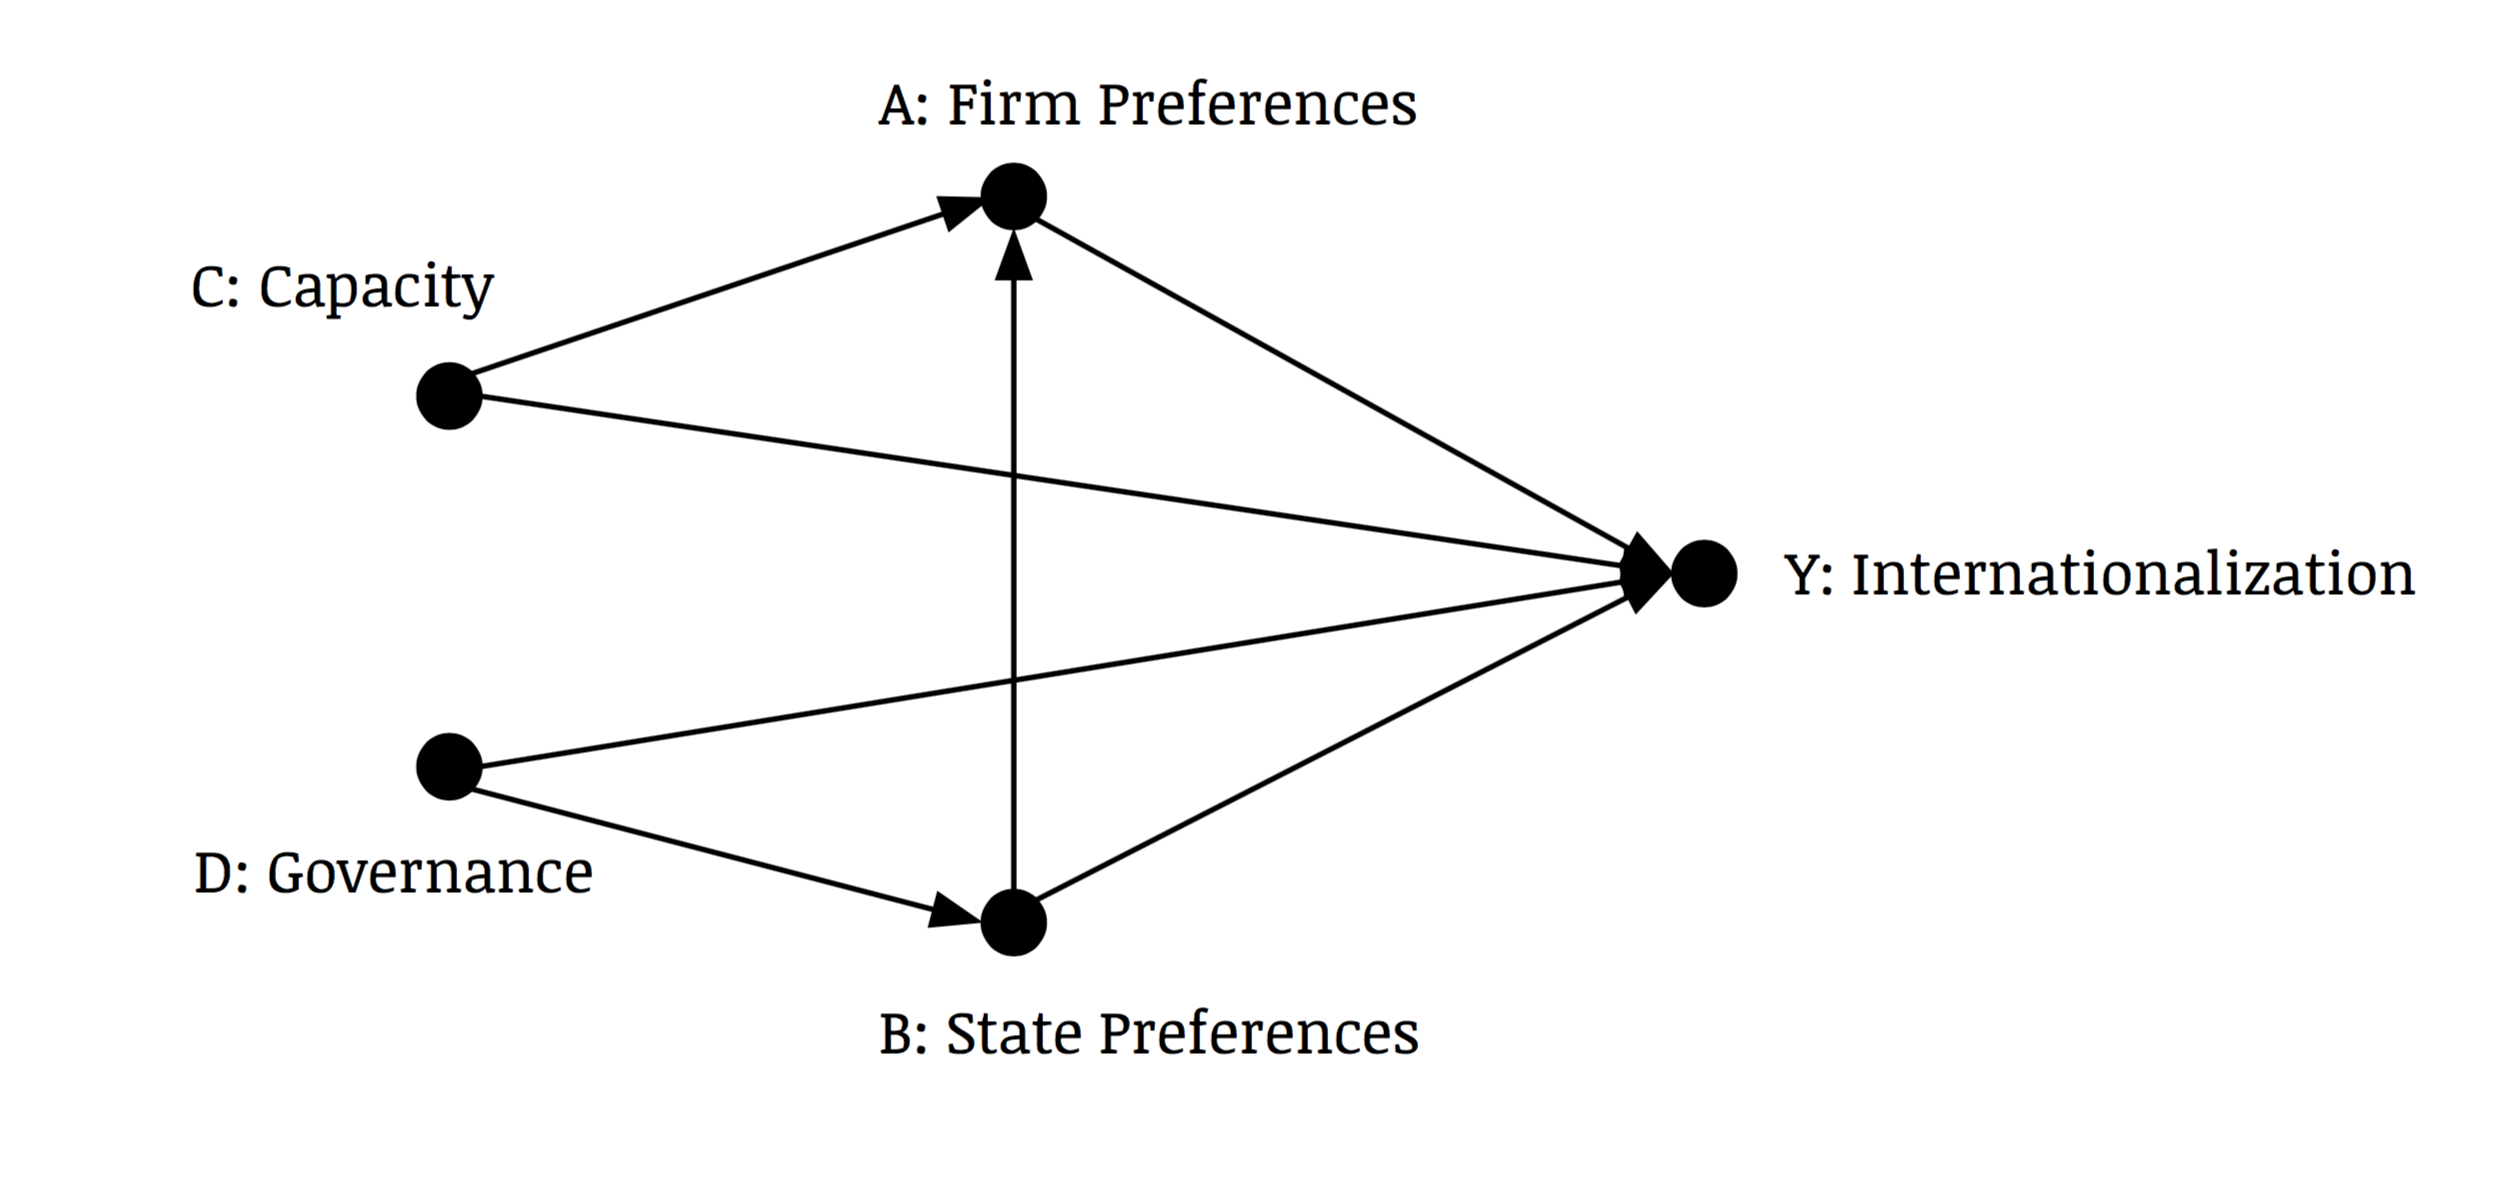
\includegraphics[width=0.5\linewidth]{fig/basic_model_2} 

}

\caption{Basic Causal Model of Internationalization}\label{fig:basicmodel}
\end{figure}

We can elaborate on the factors that influence the firm's preferences over internationalization (B) by drawing on the arguments and expert knowledge identified earlier. First, the state capacity argument suggests that a firm's perspective on internationalization will be shaped by its capacity, in so far as more capable or commercially-viable firms stand to secure and benefit from the advantages of internationalization (eg. diversification). \textbf{Firm Capacity (C)} may influence both firm and state preferences and use those as a path to affecting internationalization (C \(\rightarrow\) A \textbar{} B \(\rightarrow\) Y), but it could also affect internationalization directly by changing how other actors view, incentivize, or disincentivize internationalization (C \(\rightarrow\) Y).

State-owned firms also operate in a regulatory and governance environment that may have a significant influence on how that firm goes to market and makes decisions regarding internationalization. \textbf{Governance (D)} captures the role that the various formal or institutional organs of state oversight and influence play in the causal process. Governance is at the core of much of the political economy work focused on NOC internationalization. The bureaucratic rules could shape internationalization outcomes directly (D \(\rightarrow\) Y) or could operate indirectly by shaping firm Capacity (D \(\rightarrow\) C \(\rightarrow\) Y), firm preferences (D \(\rightarrow\) A \(\rightarrow\) Y), or state preferences (D \(\rightarrow\) B \(\rightarrow\) Y). Together, our updated causal model that incorporates the potential effects of firm capacity and governance is captured in figure \ref{fig:basicmodel}

Firm Capacity and Governance are themselves potentially influenced important variables. \textbf{Resource Wealth (E)} has the potential to causally affect firm preferences directly (as a key data input to it's decision-making) or through the firm capacity by influencing how the firm has developed over time to be more or less commercially-oriented (E \(\rightarrow\) C). Jones Luong and Sierra (2015) argue that a firm's \textbf{nationalization legacy (F)} will impact internationalization by modifying whether the firm has access to key techological resources and expertise (F \(\rightarrow\) Y). They also make the case that early firm state preference alignment is important, which in our model has a contemporary effect on the internationalization process by potentially affecting how the governance relationship has been shaped (F \(\rightarrow\) D). Cheon (2019) argues that the nature of the political system will also have an impact by shaping the support the state gives the firm: \textbf{autocracies (G)} will, all else equal, supply the firm with more direct (and directed) support for internationalization (G \(\rightarrow\) B). However, the system of governance is also likely to have shaped the nationalization process (G \(\rightarrow\) F) and the governance structure in place (G \(\rightarrow\) D). In turn, there is a substantial literature that indicates resource wealth could shape political/institutional outcomes (E \(\rightarrow\) G) and the type of nationalization seen (E \(\rightarrow\) F). Our full causal model is represented in Figure \ref{fig:fullmodel}. Crucially, the nodes A, B, and F are represented by unfilled points: these are unobserved variables in our model.

\begin{figure}

{\centering 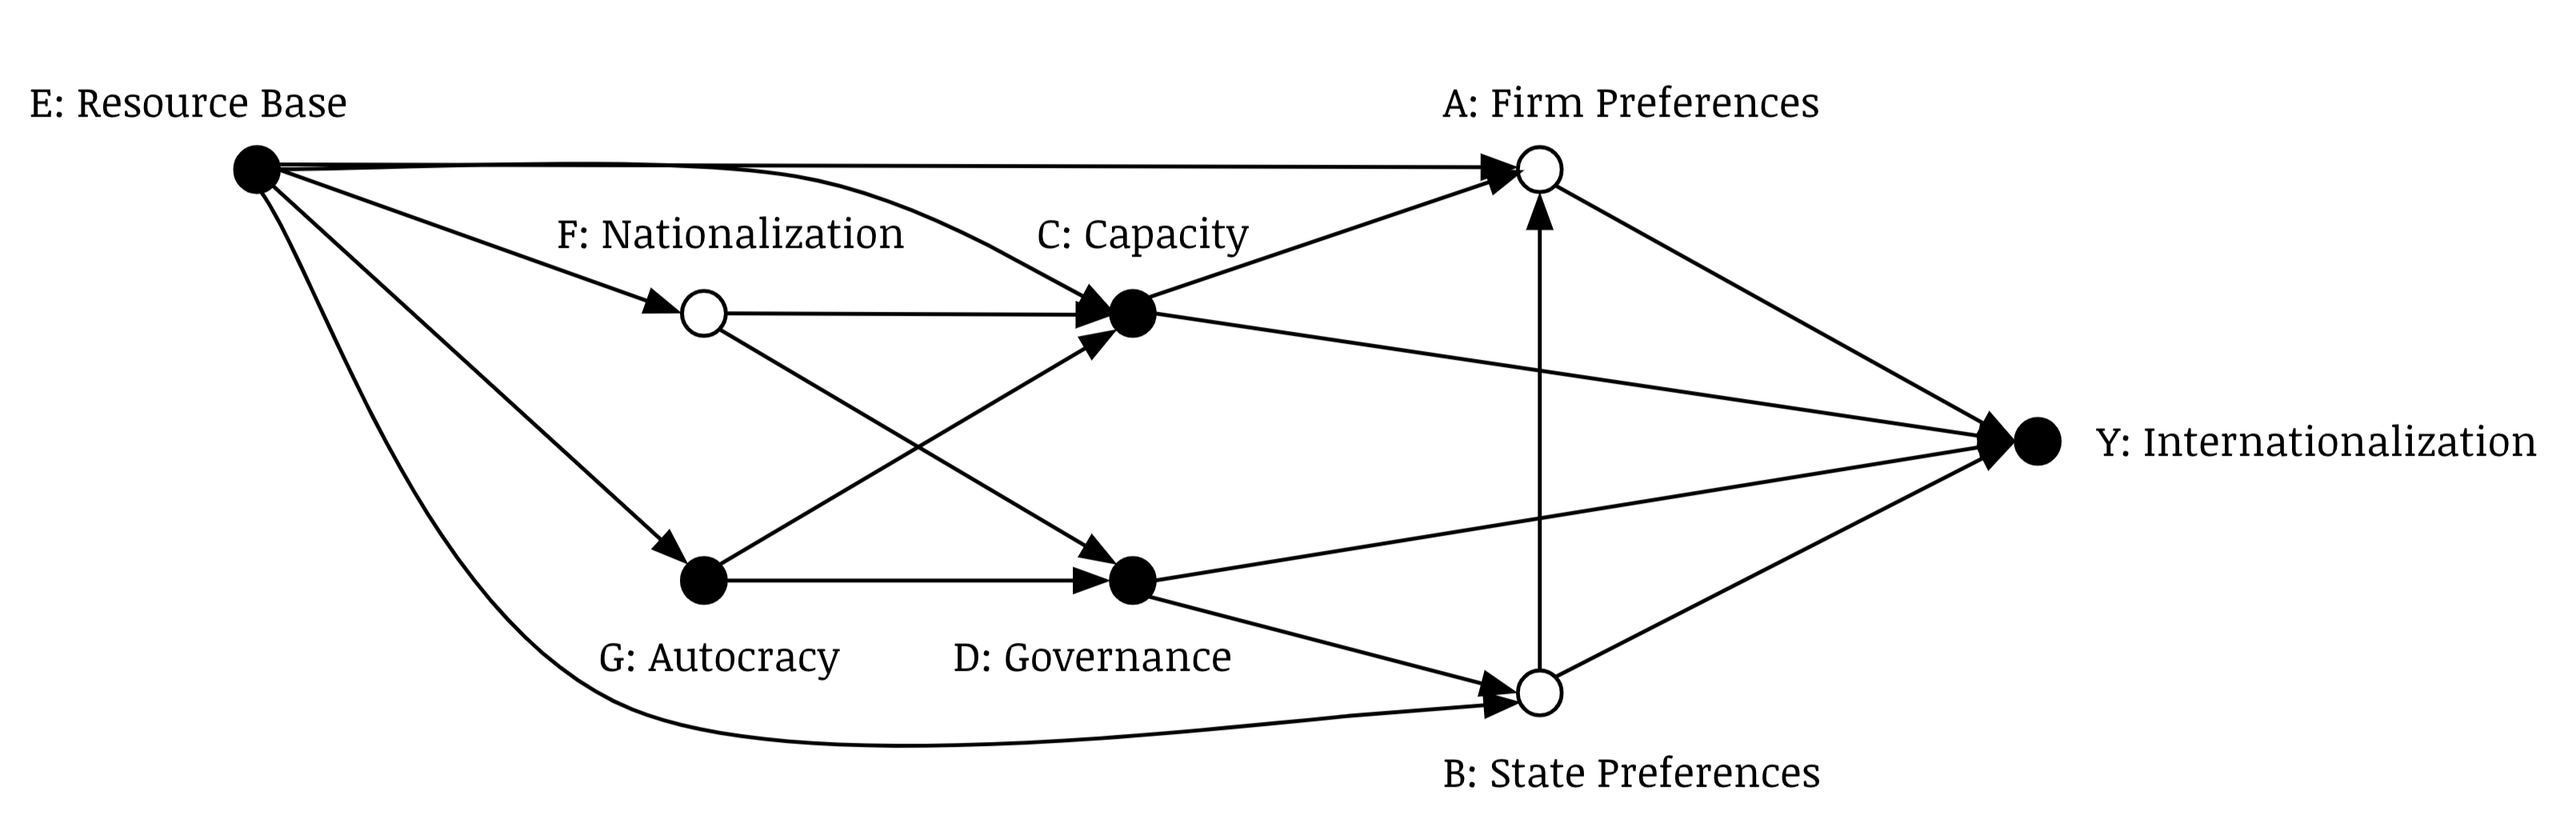
\includegraphics[width=0.8\linewidth]{fig/full_model} 

}

\caption{Full Causal Model of Internationalization}\label{fig:fullmodel}
\end{figure}

Based on the structure of our model given above, we can draw conclusions about identifiability. First, the model is causally identified: the adjustment set sufficient to block all back-door non-causal paths (thereby meeting the adjustment criterion) and identify the total effect on NOC internationalization is {[}C,D,G,E{]}. Second, we can potentially use a series of regressions to empirically evaluate the relative importance of each variable. Firm Capacity (C) and Governance (D) are all identified in the model, meaning we can give a causal interpretation to these coefficients. Resources (E) and Autocracy (G) are not identified in this model given that in both cases we condition on their descendants: they function to block back-door paths to the outcome, but are non-causal associations given the structure of the model. However, we are able to estimate the total effect of each of these variables in distinct regressions. The adjustment set sufficient to identify the total effect of Autocracy on NOC Internationalization is {[}E{]}, and the total effect of Resources on Internationalization can be measured in a simple bivariate regression, no adjustment necessary. The following section explores the measurement necessary to empirically evaluate this model, proceeds to executing and analyzing the regressions identified above.\footnote{Assessing the causal identification of this model was performed using the \texttt{Dagitty} \texttt{R} package and online interface (Textor et al. \protect\hyperlink{ref-textor_robust_2016}{2016}). The model can be found here: \url{dagitty.net/mBQp_cy}.}

\hypertarget{analysis02}{%
\section{Analysis:}\label{analysis02}}

To do for this section:

\begin{itemize}
\tightlist
\item
  Familiarize myself with some applied DAG work, preferably political science
\item
  Subsection: defining variables
\item
  Subsection: model specification
\item
  Analysis: model development
\item
  Analysis: results table
\item
  Analysis: marginal effects plot
\item
  Subsection: model discussion
\end{itemize}

\hypertarget{measurment-variable-selection}{%
\subsection{Measurment \& Variable Selection}\label{measurment-variable-selection}}

All variables scaled prior to inclusion in regression results.

\textbf{Internationalization (Outcome Variable)}: the number of international subsidiaries at the country level. Where a country has more than one NOC, average internaitonal subsidiaries is calculated.

\textbf{Firm Capacity}: proxied by the number of domestic subsidiaries a given firm has, based on the logic that more commercially viable firms will have more domestic subsidiaries, all else equal.

\textbf{State Control}: taken from Paasha Mahdavis NOC codebook. Missing data replaced with the middle value (2.5).

\textbf{Polity2 Score}: standard measure of democracy

\textbf{EIA Proven Oil Reserves}: avg. annual proven oil reserves, 1980-1990. Where there is no data in this time period, we replace null values with the proven oil reserves in 2000.

\hypertarget{raw-analysis}{%
\subsection{Raw Analysis}\label{raw-analysis}}

\begin{Shaded}
\begin{Highlighting}[]
\NormalTok{base <-}\StringTok{ }\NormalTok{subsidiaries }\OperatorTok\StringTok{ }
\StringTok{  }\KeywordTok{count}\NormalTok{(shortname, ccode, ccodecow, Status, Type) }\OperatorTok
\StringTok{  }\KeywordTok{filter}\NormalTok{(}\OperatorTok{!}\KeywordTok{is.na}\NormalTok{(Status)) }\OperatorTok\StringTok{ }
\StringTok{  }\KeywordTok{spread}\NormalTok{(Status, n) }\OperatorTok\StringTok{ }
\StringTok{  }\KeywordTok{mutate}\NormalTok{(}\DataTypeTok{domestic =} \KeywordTok{ifelse}\NormalTok{(}\KeywordTok{is.na}\NormalTok{(domestic), }\DecValTok{1}\NormalTok{, domestic)) }\OperatorTok\StringTok{ }
\StringTok{  }\KeywordTok{mutate}\NormalTok{(}\DataTypeTok{international =} \KeywordTok{ifelse}\NormalTok{(}\KeywordTok{is.na}\NormalTok{(international), }\DecValTok{0}\NormalTok{, international)) }\OperatorTok\StringTok{ }
\StringTok{  }\KeywordTok{filter}\NormalTok{(Type }\OperatorTok{==}\StringTok{ "NOC"}\NormalTok{) }\OperatorTok
\StringTok{  }\KeywordTok{group_by}\NormalTok{(ccode, ccodecow) }\OperatorTok
\StringTok{  }\KeywordTok{summarize}\NormalTok{(}\DataTypeTok{domestic =} \KeywordTok{mean}\NormalTok{(domestic),}
            \DataTypeTok{international =} \KeywordTok{mean}\NormalTok{(international)) }\OperatorTok
\StringTok{  }\KeywordTok{left_join}\NormalTok{(., state_lookup }\OperatorTok\StringTok{ }\KeywordTok{select}\NormalTok{(}\OperatorTok{-}\NormalTok{country)) }\OperatorTok
\StringTok{  }\KeywordTok{distinct}\NormalTok{() }\OperatorTok
\StringTok{  }\KeywordTok{rename}\NormalTok{(}\DataTypeTok{country =}\NormalTok{ country_new) }\OperatorTok\StringTok{ }
\StringTok{  }\KeywordTok{select}\NormalTok{(country, ccode, ccodecow, international, domestic, fh_polity2)}
\end{Highlighting}
\end{Shaded}

\begin{Shaded}
\begin{Highlighting}[]
\NormalTok{df <-}\StringTok{ }\NormalTok{subsidiaries }\OperatorTok\StringTok{ }
\StringTok{  }\KeywordTok{count}\NormalTok{(shortname, ccode, ccodecow, Status, Type) }\OperatorTok
\StringTok{  }\KeywordTok{filter}\NormalTok{(}\OperatorTok{!}\KeywordTok{is.na}\NormalTok{(Status)) }\OperatorTok\StringTok{ }
\StringTok{  }\KeywordTok{spread}\NormalTok{(Status, n) }\OperatorTok
\StringTok{  }\KeywordTok{mutate}\NormalTok{(}\DataTypeTok{domestic =} \KeywordTok{ifelse}\NormalTok{(}\KeywordTok{is.na}\NormalTok{(domestic), }\DecValTok{1}\NormalTok{, domestic)) }\OperatorTok\StringTok{ }
\StringTok{  }\KeywordTok{mutate}\NormalTok{(}\DataTypeTok{international =} \KeywordTok{ifelse}\NormalTok{(}\KeywordTok{is.na}\NormalTok{(international), }\DecValTok{0}\NormalTok{, international)) }\OperatorTok\StringTok{ }
\StringTok{  }\KeywordTok{filter}\NormalTok{(Type }\OperatorTok{==}\StringTok{ "NOC"}\NormalTok{) }\OperatorTok
\StringTok{  }\KeywordTok{group_by}\NormalTok{(ccode, ccodecow) }\OperatorTok
\StringTok{  }\KeywordTok{summarize}\NormalTok{(}\DataTypeTok{domestic =} \KeywordTok{mean}\NormalTok{(domestic),}
            \DataTypeTok{international =} \KeywordTok{mean}\NormalTok{(international)) }\OperatorTok
\StringTok{  }\KeywordTok{left_join}\NormalTok{(., state_lookup }\OperatorTok\StringTok{ }\KeywordTok{select}\NormalTok{(}\OperatorTok{-}\NormalTok{country)) }\OperatorTok
\StringTok{  }\KeywordTok{distinct}\NormalTok{() }\OperatorTok
\StringTok{  }\KeywordTok{rename}\NormalTok{(}\DataTypeTok{country =}\NormalTok{ country_new) }\OperatorTok\StringTok{ }
\StringTok{  }\KeywordTok{select}\NormalTok{(country, ccode, ccodecow, international, domestic,}
\NormalTok{         dr_eg, bti_ep, bti_gp, bti_gi, icrg_qog, fh_polity2, }
\NormalTok{         wdi_oilrent, ross_oil_prod) }\OperatorTok
\StringTok{  }\KeywordTok{left_join}\NormalTok{(.,}
            \KeywordTok{read_csv}\NormalTok{(}\StringTok{"data/raw/EIA_International_data.csv"}\NormalTok{, }\DataTypeTok{na =} \KeywordTok{c}\NormalTok{(}\OtherTok{NA}\NormalTok{, }\StringTok{"--"}\NormalTok{)) }\OperatorTok
\StringTok{              }\KeywordTok{gather}\NormalTok{(Year, oil, }\DecValTok{2}\OperatorTok{:}\DecValTok{12}\NormalTok{) }\OperatorTok
\StringTok{              }\KeywordTok{mutate}\NormalTok{(}\DataTypeTok{reserves =} \KeywordTok{as.numeric}\NormalTok{(oil)) }\OperatorTok
\StringTok{              }\KeywordTok{group_by}\NormalTok{(country) }\OperatorTok\StringTok{ }
\StringTok{              }\KeywordTok{summarize}\NormalTok{(}\DataTypeTok{reserves =} \KeywordTok{mean}\NormalTok{(reserves, }\DataTypeTok{na.rm =}\NormalTok{ T)) }\OperatorTok
\StringTok{              }\KeywordTok{na.omit}\NormalTok{() }\OperatorTok
\StringTok{              }\KeywordTok{mutate}\NormalTok{(}\DataTypeTok{country =} \KeywordTok{case_when}\NormalTok{(country }\OperatorTok{==}\StringTok{ "Sudan"} \OperatorTok{~}\StringTok{ "Sudan (2012-)"}\NormalTok{,}
\NormalTok{                                         country }\OperatorTok{==}\StringTok{ "Pakistan"} \OperatorTok{~}\StringTok{ "Pakistan (1971-)"}\NormalTok{,}
\NormalTok{                                         country }\OperatorTok{==}\StringTok{ "Malaysia"} \OperatorTok{~}\StringTok{ "Malaysia (1966-)"}\NormalTok{,}
\NormalTok{                                         country }\OperatorTok{==}\StringTok{ "Cote dIvoire (IvoryCoast)"} \OperatorTok{~}\StringTok{ "Cote d'Ivoire"}\NormalTok{,}
\NormalTok{                                         country }\OperatorTok{==}\StringTok{ "Congo (Kinshasa)"} \OperatorTok{~}\StringTok{ "Congo, Democratic Republic"}\NormalTok{,}
                                         \OtherTok{TRUE} \OperatorTok{~}\StringTok{ }\NormalTok{country)) }\OperatorTok
\StringTok{              }\KeywordTok{right_join}\NormalTok{(., base }\OperatorTok\StringTok{ }\KeywordTok{select}\NormalTok{(country, ccode)) }\OperatorTok
\StringTok{              }\KeywordTok{left_join}\NormalTok{(., }\KeywordTok{read_csv}\NormalTok{(}\StringTok{"data/raw/International_data_2000.csv"}\NormalTok{, }\DataTypeTok{na =} \KeywordTok{c}\NormalTok{(}\OtherTok{NA}\NormalTok{, }\StringTok{"--"}\NormalTok{)) }\OperatorTok
\StringTok{                          }\KeywordTok{mutate}\NormalTok{(}\DataTypeTok{reserves_2000 =} \KeywordTok{as.numeric}\NormalTok{(reserves_}\DecValTok{2000}\NormalTok{))) }\OperatorTok
\StringTok{              }\KeywordTok{mutate}\NormalTok{(}\DataTypeTok{reserves =} \KeywordTok{ifelse}\NormalTok{(}\KeywordTok{is.na}\NormalTok{(reserves), reserves_}\DecValTok{2000}\NormalTok{, reserves))) }\OperatorTok\StringTok{ }
\StringTok{  }\KeywordTok{left_join}\NormalTok{(., readxl}\OperatorTok{::}\KeywordTok{read_excel}\NormalTok{(}\StringTok{"data/raw/noc_var.xlsx"}\NormalTok{) }\OperatorTok\StringTok{ }
\StringTok{              }\KeywordTok{select}\NormalTok{(ccode, control) }\OperatorTok\StringTok{ }
\StringTok{              }\KeywordTok{na.omit}\NormalTok{() }\OperatorTok
\StringTok{              }\KeywordTok{rename}\NormalTok{(}\DataTypeTok{ccodecow =}\NormalTok{ ccode)) }\OperatorTok
\StringTok{  }\KeywordTok{distinct}\NormalTok{() }\OperatorTok
\StringTok{  }\KeywordTok{mutate}\NormalTok{(}\DataTypeTok{control =} \KeywordTok{ifelse}\NormalTok{(}\KeywordTok{is.na}\NormalTok{(control), }\FloatTok{2.5}\NormalTok{, control))}

\NormalTok{df}\OperatorTok{$}\NormalTok{i_scaled <-}\StringTok{ }\KeywordTok{scale}\NormalTok{(df}\OperatorTok{$}\NormalTok{international)}
\NormalTok{df}\OperatorTok{$}\NormalTok{d_scaled <-}\StringTok{ }\KeywordTok{scale}\NormalTok{(df}\OperatorTok{$}\NormalTok{domestic)}
\NormalTok{df}\OperatorTok{$}\NormalTok{c_scaled <-}\StringTok{ }\KeywordTok{scale}\NormalTok{(df}\OperatorTok{$}\NormalTok{control)}
\NormalTok{df}\OperatorTok{$}\NormalTok{p_scaled <-}\StringTok{ }\KeywordTok{scale}\NormalTok{(df}\OperatorTok{$}\NormalTok{fh_polity2)}
\NormalTok{df}\OperatorTok{$}\NormalTok{r_scaled <-}\StringTok{ }\KeywordTok{scale}\NormalTok{(df}\OperatorTok{$}\NormalTok{reserves)}
\end{Highlighting}
\end{Shaded}

\begin{Shaded}
\begin{Highlighting}[]
\NormalTok{broom}\OperatorTok{::}\KeywordTok{tidy}\NormalTok{(}\KeywordTok{summary}\NormalTok{(}\KeywordTok{lm}\NormalTok{(i_scaled }\OperatorTok{~}\StringTok{ }
\StringTok{             }\NormalTok{d_scaled }\OperatorTok{+}\StringTok{ }
\StringTok{             }\NormalTok{c_scaled }\OperatorTok{+}\StringTok{ }
\StringTok{             }\NormalTok{p_scaled }\OperatorTok{+}\StringTok{ }
\StringTok{             }\NormalTok{r_scaled, }
           \DataTypeTok{data =}\NormalTok{ df)))}
\end{Highlighting}
\end{Shaded}

\begin{verbatim}
## # A tibble: 5 x 5
##   term         estimate std.error statistic  p.value
##   <chr>           <dbl>     <dbl>     <dbl>    <dbl>
## 1 (Intercept) -9.90e-17     0.113 -8.76e-16 1.00    
## 2 d_scaled     4.64e- 1     0.115  4.04e+ 0 0.000160
## 3 c_scaled    -5.83e- 2     0.121 -4.81e- 1 0.633   
## 4 p_scaled     2.10e- 1     0.123  1.70e+ 0 0.0944  
## 5 r_scaled     1.15e- 1     0.128  9.00e- 1 0.372
\end{verbatim}

\begin{Shaded}
\begin{Highlighting}[]
\KeywordTok{sd}\NormalTok{(df}\OperatorTok{$}\NormalTok{international)}
\end{Highlighting}
\end{Shaded}

\begin{verbatim}
## [1] 54.13521
\end{verbatim}

\begin{Shaded}
\begin{Highlighting}[]
\KeywordTok{sd}\NormalTok{(df}\OperatorTok{$}\NormalTok{domestic)}
\end{Highlighting}
\end{Shaded}

\begin{verbatim}
## [1] 70.00283
\end{verbatim}

\begin{Shaded}
\begin{Highlighting}[]
\KeywordTok{summary}\NormalTok{(}\KeywordTok{lm}\NormalTok{(i_scaled }\OperatorTok{~}\StringTok{ }\NormalTok{r_scaled, }\DataTypeTok{data =}\NormalTok{ df))}
\end{Highlighting}
\end{Shaded}

\begin{verbatim}
## 
## Call:
## lm(formula = i_scaled ~ r_scaled, data = df)
## 
## Residuals:
##     Min      1Q  Median      3Q     Max 
## -0.7232 -0.6311 -0.4749  0.2961  4.9926 
## 
## Coefficients:
##               Estimate Std. Error t value Pr(>|t|)
## (Intercept) -4.280e-17  1.268e-01    0.00     1.00
## r_scaled     6.005e-02  1.278e-01    0.47     0.64
## 
## Residual standard error: 1.006 on 61 degrees of freedom
## Multiple R-squared:  0.003606,   Adjusted R-squared:  -0.01273 
## F-statistic: 0.2208 on 1 and 61 DF,  p-value: 0.6401
\end{verbatim}

\begin{Shaded}
\begin{Highlighting}[]
\KeywordTok{summary}\NormalTok{(}\KeywordTok{lm}\NormalTok{(i_scaled }\OperatorTok{~}\StringTok{ }\NormalTok{p_scaled }\OperatorTok{+}\StringTok{ }\NormalTok{r_scaled, }\DataTypeTok{data =}\NormalTok{ df))}
\end{Highlighting}
\end{Shaded}

\begin{verbatim}
## 
## Call:
## lm(formula = i_scaled ~ p_scaled + r_scaled, data = df)
## 
## Residuals:
##     Min      1Q  Median      3Q     Max 
## -0.7885 -0.6325 -0.3869  0.3728  4.8010 
## 
## Coefficients:
##               Estimate Std. Error t value Pr(>|t|)
## (Intercept) -5.595e-17  1.261e-01   0.000    1.000
## p_scaled     1.752e-01  1.366e-01   1.282    0.205
## r_scaled     1.242e-01  1.366e-01   0.909    0.367
## 
## Residual standard error: 1.001 on 60 degrees of freedom
## Multiple R-squared:  0.03017,    Adjusted R-squared:  -0.002156 
## F-statistic: 0.9333 on 2 and 60 DF,  p-value: 0.3989
\end{verbatim}

\begin{Shaded}
\begin{Highlighting}[]
\NormalTok{m1 <-}\StringTok{ }\KeywordTok{lm}\NormalTok{(i_scaled }\OperatorTok{~}\StringTok{ }\NormalTok{d_scaled }\OperatorTok{+}\StringTok{ }\NormalTok{c_scaled }\OperatorTok{+}\StringTok{ }\NormalTok{p_scaled }\OperatorTok{+}\StringTok{ }\NormalTok{r_scaled, }\DataTypeTok{data =}\NormalTok{ df)}
\NormalTok{m2 <-}\StringTok{ }\KeywordTok{lm}\NormalTok{(i_scaled }\OperatorTok{~}\StringTok{ }\NormalTok{p_scaled }\OperatorTok{+}\StringTok{ }\NormalTok{r_scaled, }\DataTypeTok{data =}\NormalTok{ df)}
\NormalTok{m3 <-}\StringTok{ }\KeywordTok{lm}\NormalTok{(i_scaled }\OperatorTok{~}\StringTok{ }\NormalTok{r_scaled, }\DataTypeTok{data =}\NormalTok{ df)}
\end{Highlighting}
\end{Shaded}

\begin{Shaded}
\begin{Highlighting}[]
\NormalTok{stargazer}\OperatorTok{::}\KeywordTok{stargazer}\NormalTok{(m1, m2, m3, }
          \DataTypeTok{covariate.labels =} \KeywordTok{c}\NormalTok{(}\StringTok{"Firm Capacity"}\NormalTok{, }
                               \StringTok{"State Control"}\NormalTok{, }
                               \StringTok{"Polity2 Score"}\NormalTok{, }
                               \StringTok{"Oil Reserves"}\NormalTok{),}
          \DataTypeTok{dep.var.labels   =} \StringTok{"Number of International Subsidiaries"}\NormalTok{,}
          \DataTypeTok{type=}\StringTok{'latex'}\NormalTok{)}
\end{Highlighting}
\end{Shaded}

\% Table created by stargazer v.5.2.2 by Marek Hlavac, Harvard University. E-mail: hlavac at fas.harvard.edu
\% Date and time: Thu, Jun 25, 2020 - 13:41:39

\begin{table}[!htbp] \centering 
  \caption{} 
  \label{} 
\begin{tabular}{@{\extracolsep{5pt}}lccc} 
\\[-1.8ex]\hline 
\hline \\[-1.8ex] 
 & \multicolumn{3}{c}{\textit{Dependent variable:}} \\ 
\cline{2-4} 
\\[-1.8ex] & \multicolumn{3}{c}{Number of International Subsidiaries} \\ 
\\[-1.8ex] & (1) & (2) & (3)\\ 
\hline \\[-1.8ex] 
 Firm Capacity & 0.464$^{***}$ &  &  \\ 
  & (0.115) &  &  \\ 
  & & & \\ 
 State Control & $-$0.058 &  &  \\ 
  & (0.121) &  &  \\ 
  & & & \\ 
 Polity2 Score & 0.210$^{*}$ & 0.175 &  \\ 
  & (0.123) & (0.137) &  \\ 
  & & & \\ 
 Oil Reserves & 0.115 & 0.124 & 0.060 \\ 
  & (0.128) & (0.137) & (0.128) \\ 
  & & & \\ 
 Constant & $-$0.000 & $-$0.000 & $-$0.000 \\ 
  & (0.113) & (0.126) & (0.127) \\ 
  & & & \\ 
\hline \\[-1.8ex] 
Observations & 63 & 63 & 63 \\ 
R$^{2}$ & 0.248 & 0.030 & 0.004 \\ 
Adjusted R$^{2}$ & 0.196 & $-$0.002 & $-$0.013 \\ 
Residual Std. Error & 0.897 (df = 58) & 1.001 (df = 60) & 1.006 (df = 61) \\ 
F Statistic & 4.784$^{***}$ (df = 4; 58) & 0.933 (df = 2; 60) & 0.221 (df = 1; 61) \\ 
\hline 
\hline \\[-1.8ex] 
\textit{Note:}  & \multicolumn{3}{r}{$^{*}$p$<$0.1; $^{**}$p$<$0.05; $^{***}$p$<$0.01} \\ 
\end{tabular} 
\end{table}

Coefficient on scaled ``capacity'' : 0.46. Coefficient on scaled control : -0.058. Scaling: The result is that the values in the transformed variable have the same relationship to one another as in the untransformed variable, but the transformed variable has mean 0 and standard deviation 1 Interpretation: The effect of scaled capacity (d\_scaled) now represents the expected change in standard deviations of internationalization for a 1-standard-deviation increase in capacity; that is, for a 1-SD increase in capacity, we expect a 0.46-SD decrease in internationalization, which we could call an effect of moderate magnitude. Substantive effects: an increase of 70 domestic subsidiaries should lead to an increase of 54 international subsidiaries, all else equal.

\begin{Shaded}
\begin{Highlighting}[]
\NormalTok{broom}\OperatorTok{::}\KeywordTok{tidy}\NormalTok{(m1) }\OperatorTok
\StringTok{  }\NormalTok{dotwhisker}\OperatorTok{::}\KeywordTok{relabel_predictors}\NormalTok{(}\KeywordTok{c}\NormalTok{(}\DataTypeTok{d_scaled =} \StringTok{"Firm Capacity"}\NormalTok{,}
                       \DataTypeTok{c_scaled =} \StringTok{"State Control"}\NormalTok{,}
                       \DataTypeTok{p_scaled =} \StringTok{"Polity2 Score"}\NormalTok{,}
                       \DataTypeTok{r_scaled =} \StringTok{"Oil Reserves"}\NormalTok{)) }\OperatorTok\StringTok{ }
\StringTok{  }\NormalTok{dotwhisker}\OperatorTok{::}\KeywordTok{dwplot}\NormalTok{() }\OperatorTok{+}
\StringTok{  }\KeywordTok{geom_vline}\NormalTok{(}\DataTypeTok{xintercept =} \DecValTok{0}\NormalTok{, }\DataTypeTok{color =} \StringTok{"grey30"}\NormalTok{, }\DataTypeTok{linetype =} \DecValTok{3}\NormalTok{) }\OperatorTok{+}
\StringTok{  }\KeywordTok{xlim}\NormalTok{(}\OperatorTok{-}\DecValTok{1}\NormalTok{,}\DecValTok{1}\NormalTok{) }\OperatorTok{+}
\StringTok{  }\KeywordTok{labs}\NormalTok{(}\DataTypeTok{x =} \StringTok{"Coefficient Estimate, Scaled"}\NormalTok{) }\OperatorTok{+}
\StringTok{  }\KeywordTok{scale_color_grey}\NormalTok{() }\OperatorTok{+}
\StringTok{  }\KeywordTok{theme_bw}\NormalTok{() }\OperatorTok{+}
\StringTok{  }\KeywordTok{theme}\NormalTok{(}\DataTypeTok{legend.position =} \StringTok{"none"}\NormalTok{)}
\end{Highlighting}
\end{Shaded}

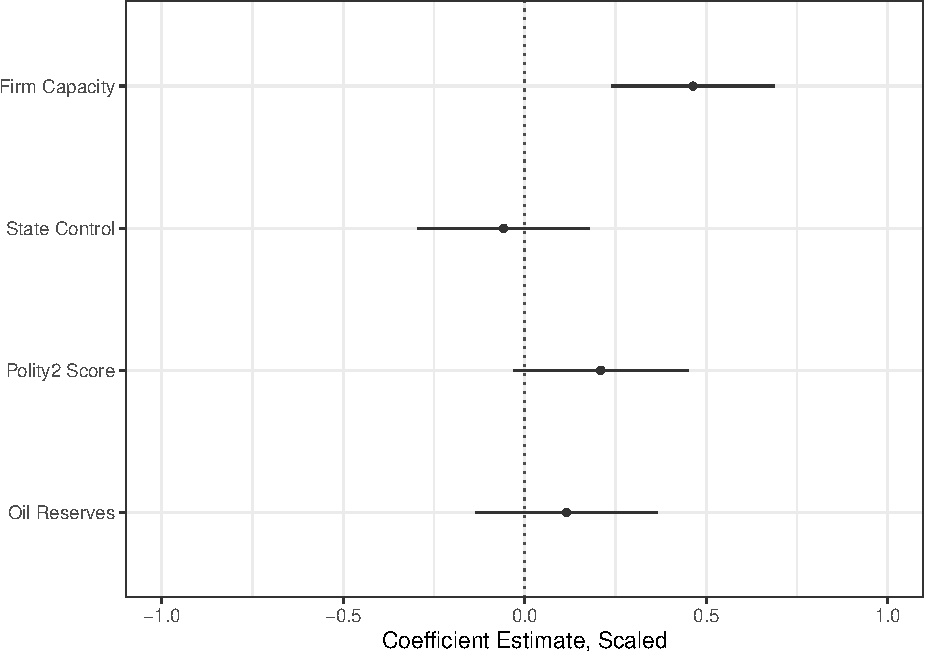
\includegraphics{finalfig/basemodelplot-1.pdf}

\hypertarget{paper3}{%
\chapter{The politics of NOC internationalization}\label{paper3}}

\hypertarget{intro03}{%
\section{Introduction}\label{intro03}}

\begin{quote}
\textbf{Due to its geographical location and proximity to Russia, Tajikistan is of strategic interest to Russia and, correspondingly, the Gazprom Group.} Gazprom is interested in preserving the stable economic situation in Central Asia in general and Tajikistan in particular. Therefore, Gazprom is both a strategic partner to Tajikistan as well as its largest investor. The Group's main objective in Tajikistan, besides purely commercial profit, is to guarantee the energy security of the republic, at a time when the country's economy is experiencing a serious shortage of oil and gas.\footnote{Gazprom International: Tajikistan (Country Profile). \url{http://www.gazprom-international.com/en/operations/country/tajikistan}}
\end{quote}

The politics of NOC internationalization is often the most discussed aspect of a particular investment or acqusition. Popular observers and concerned politicians regularly argue that a particular deal is politically motivated or comes with political strings attached.\footnote{For example, see the discussion int the popular press surrounding CNOOC's potential acquisition of UNOCAL. \textbf{example cite needed}.} A 2007 Congressional Report on NOCs listed foreign policy as a core objective: ``National oil companies can also be used by their national governments as a tool to achieve foreign policy goals, leading to direct alliances as well as {[}firm to firm{]} ties that can pave the way to political relationships. Oil is a strategic commodity in the world economy, and its production and use can foster strategic relationships.'' (Pirog \protect\hyperlink{ref-pirog_role_2007}{2007}, 7--8).

Statements made by the investing firm or state that confirm this --- like the one above, found on a public Gazprom website --- are harder to come by. It seems obvious that the activities engaged in by a state's largest economic entity will necessarily have political implications and impacts, but getting an empirical handle on those implications and impacts is difficult. Justifications for a particular investment decision or location choice can always be made by appealing to a purely commercial logic; the relationships woven between political actors through a web of commercial/contractual relationships are almost necessarily subtle and subtextual rather than explicit or codified. As such, research into the political implications of the commercial relationships formed when national oil companies (NOCs) build out an international network are few in number and limited in scope.

At the same time, however, the topic is highly deserving of more rigorous empirical attention. In many cases, a state's national oil company is the crown jewel of the state's economic and social apparatus. It stands to reason that political owners may be highly invested in the international activity of their firms for both commercial and political reasons. Acquisitions and investments open doors that diplomats are involved in both creating and leveraging once in place. There is a reason that the highest level of political dignitary have been involved in the announcement and opening of many China's most significant investments in Africa.\footnote{\textbf{TODO: insert China Africa cite here}.} When it comes to international expansion, the state-firm relationship can be mutually beneficial. As the chair of an Indian NOC states, ``diplomatic support is very, very crucial as we search for assets overseas.''\footnote{Kakatey (\protect\hyperlink{ref-kakatey_india_2010}{2010}), quoted in Meckling, Kong, and Madan (\protect\hyperlink{ref-meckling_oil_2015}{2015}), 1180.}

This chapter addresses the political implications of NOC internationalization in three moves. First, we make `political implications' specific by enumerating several of the most important ways that NOC internationalization can have aspects and implications beyond the purely commercial. We group these into a typology of political internationalization, and group each component into home state, host state, and firm-specific categories. We substantiate these implications with sailient anecdotes. Our objective with this section is to be as specific and explict as possible about the the potential shape of the political in the context of NOC internationalization.

Second, we describe and investigate the web of state-to-state relationships that emerge from internationalization activities of NOCs across the globe. We argue that subsidiary networks emerge in measurably distinct forms: these networks can be used to distinguish NOCs from IOCs, but also to distinguish between different kinds of NOCs. \textbf{TODO: More detail on this one here.}

Third, we attempt to gain leverage over the causal effect of NOC internationalization by examining key internationalization events and their impacts over time. Our approach combines careful attention to causal inference in the context of time-varying outcomes with statistical techniques --- specifically, diffusion-regression state-space modeling --- designed to gain leverage over the causal impact of a treatment over time in both experimental and observational settings.

\hypertarget{motiv03}{%
\section{Motivation: The Politics of Internationalization}\label{motiv03}}

What does it mean to say that the international activity of NOCs has political implications? The objective of this section is to articulate some of these implications in a manner that leaves them more conducive to empirical investigation. The discussion below pursues one specific way of conceptualizing these implitcations: it makes the case that \textbf{NOC internationalization is political insofar as it generates (or is expected to generate) political outcomes for the parent state}. These political outcomes include (but are likely not limited to) improved state-to-state relationships, amplified international signalling, and strengthened international trade flows.

While this section pursues a focus on the international political implications of NOC internationalization for the parent state of a NOC, there are at least three other approaches deserving of further inquiry. First, NOC internationalization has political implications for the state receiving the investment or expansion activity. In some ways this is a corollary of the main thread pursued here, but it also offers significant departures. Sanctioning NOC internationalization activity by approving specific projects can have important political implications whether or not the parent state is engaged in or attentive to the firm acitvity at all. In many cases regulators grapple with the percieved costs and benefits of allowing a state-owned firm to develop operations, and in some cases the political or regulatory pushback has been significant enough to derail the efforts entirely (eg. Unocal in the United States, \textbf{more detail or footnote here}).

Second, there are political implications of international activity for NOCs themselves. They may actively leverage their political connections to open channels of access or communication, may find their commercial efforts inhibited by the political reputation of their home state, or may utilize their political backing to justify and pursue more risk-acceptant investments.

Third, international activity engaged in by NOCs likely also has implications for the parent state in the domestic sphere. Firms that grow internationally may build out more robust and valuable domestic infrastructure, changing the way the state may be able to use the proceeds or instittusions of the firm to support the domestic economy and engage in patronage of various forms.

While individually compelling, we do not pursue any of these in further theoretical or empirical detail here. We revisit them both in the discussion section that concludes these chapters, and flesh them out as some of the most promising avenues for further research into this topic. This section, and the analysis that follows, is limited in scope to the international political implications of NOC internationalization.

\hypertarget{the-intrinsic-political-importance-of-commercial-activity}{%
\subsection{The intrinsic political importance of commercial activity}\label{the-intrinsic-political-importance-of-commercial-activity}}

NOC internationalization has political implications when the state derives or expects political benefit from the NOCs performance in general, and its performance linked to investments and expansions made in particular. In this way, the purely commercial outcomes of firm activity abroad can have important political outcomes: these outcomes can help a government shore up support domestically, fund key initiatives, and engage in other politically-motivated activities. The most basic (but significant) way this operates is in NOC contributions to state treasuries: many states use their NOC profit to fund the state, and in many cases the NOC is the largest single contributor of funds. Growth in these contributions --- either because of rising oil prices, improved firm performance, or both --- plays an important role in improving the political fortunes of the elites or parties in power. State interest in the commercial outcomes delivered by their NOC's international activity goes the other way as well. International expansion is never risk free, and the state may pay a political price for poor investments or a suffering firm. Just as the state may benefit from rising contributions, shortfalls can create difficulties vis-a-vis the electorate (or selectorate).

Recent events in Venezuela illustrate how international subdidiaries can be both political \emph{assets} and \emph{liabilities}. In spring 2019 the Venezuelan government approved a controversial measure to pay overdue interest payments against the country's only remaining non-defaulted bond, PDVSA 2020 debt. This measure is going ahead, despite the desperate general state of Venezuela's finances and economy, because non-payment would open one of PEMEX's most important assets to seizure by creditors. The PEMEX 2020 bond is backed by shares in Citgo, a US refiner: its loss is a bridge too far for the Venezuelan government (Armas \protect\hyperlink{ref-armas_venezuela_2019}{2019}; Smith \protect\hyperlink{ref-smith_venezuela_2019}{2019}). Citgo is one of PEMEX's largest and most productive international subsidiaries. The Venezuelan government is willing to risk significant public outcry and balance-sheet pain in other areas of its economy to secure this valuable international asset.

Evaluating the proposition that NOC internationalization can be political by virtue of how political actors view and understand its commercial dimensions presents significant challenges. It is likely that at some level, \emph{all} deals of this nature --- ie. pursued by a state-owned entity --- likely hold at least some level of political importance for the parties involved; many non-state-owned transactions do as well. Assessing the strength or saliency of this importance from case to case is extremely difficult, and require far more nuanced data regarding the perceptions and preferences of state and firm actors than are currently available.

\hypertarget{noc-internationalization-and-bilateral-politics}{%
\subsection{NOC internationalization and bilateral politics}\label{noc-internationalization-and-bilateral-politics}}

In what ways might the international activity of NOCs generate political outcomes for their parent states, beyond the intrisic political importance of large-scale commercial transactions? First, firm activity in other countries might impact the state-to-state relationships between that country and the NOC's parent state. Firm investments are rarely made with diplomatic or strategic strings explicitly attached, but it is likely that at least in some cases, commercial deals are expected to deliver political or diplomatic value as well. This could mean that the state receiving the investment is more likely to participate in bilateral or multilateral projects, act as a regional partner for the investing firm's state, or support that state's initiatives in international forums like the United Nations.

The strong version of this expected impact is that the international link formed by the NOC can be a direct channel of influence or even coercion. The likelihood of this influence being meaningful may be higher when the receiving state becomes dependent on that relationship. In this vein, some observers view Gazprom's near-monoplist position in many European gas markets as constituting a `gas weapon': the ability of the Russian state to turn off critical supplies at moments of tension may be an important lever or influence over states that require these supplies to run their economies and supply their domestic markets effectively.\footnote{\textbf{Insert citations here.}} Supply chain relationships work in both directions, however: the supplier is often just as reliant on stability of supply, and places a high value on a commercially reliable reputation. Any understanding of a resource `weapon' must be balanced against the possibility that commercial linkages operate as `shields': creating an important asset for the investing state that they wouldn't want to risk disrupting by overly antagonistic diplomatic or strategic actions.

The more likely or common process by which NOC activities abroad impact interstate relations is as one tie among others that link the two states. A firm's investments may facilitate or improve lines of communication, coordination, and cooperation, especially when the firm is large relative to the diplomatic apparatuses of the states in question.

\textbf{Insert appropriate anecdote here: maybe India / Saudi, or China / Africa}

Alternatively, the political implications of commercial relationships formed by NOCs may operate irrespective of the active bilateral relationship between the two states. The state-owner of the investing firm may be interested in supporting the economy or general stability of another state whether or not that state's behaviour changes. The opening quote from Gazprom, situated at the beginning of this chapter, illustrates this implicaiton clearly: Russia's political interest in Gazprom's investment in Tajikistan stems in part at least from an interest in securing the stability of an important neighbour on Russia's volatile southern border. This interest likely adheres irrespective of how Tajikistan responds to Gazprom or Russia's actions.

These political implications likely adhere to other forms of commercial activity: NOCs aren't the only firms capable of generating political impacts of this nature, especially in a strategically important sector like hydrocarbon extraction and production. Political entities can invested in the activities of non-state-owned firms as well. The condition of state-ownership does create a stronger link between state and firm, however, and so it is plausible that these implications are more substantial in the context of NOC activity than in the context of activity engaged in by other multinational oil and gas companies.

Within this conceptualization, bilateral relations and firm-to-firm relations are closely bound together. States may sanction and even push firms to expand and develop international connections in ways that improve specific bilateral ties or deliver against specific political objectives. Alternatively, firms may engage in commercial activities that subsequently deliver political benefits (or costs) for the parent state.

\hypertarget{noc-internationalization-and-international-trade}{%
\subsection{NOC internationalization and international trade}\label{noc-internationalization-and-international-trade}}

Direct political ties are one form of linkage NOC activity can impact; trade ties are another. States may derive (or expect to derive) material within-sector and cross-sector benefits in the trade of both goods and services as a result of a NOC-subsidiary link being formed. In the most direct sense, NOC-subsidiary linkages enable the intra-firm exchange of goods and services. More broadly, however, the state may reasonably expect knock-on benefits resulting from improved partnerships, enabling agreements or regulatory breakthroughs, or other aspects of the link. These are likely strongest within the sector in question, but may also be felt in adjacent and even very different areas of the economy.

Illustrations of this connection in practice are readily available. Bilateral trade growth between Russia and the United Arab Emirates, for instance, covers several critical sectors, including but not limited to energy: efforts to strengthen those ties necessarily involve ADNOC CEO and Minister of State Sultan Al Jaber.\footnote{``Russia, UAE trade ties on upswing'', \emph{Gulf Times}, \url{https://gulfnews.com/business/markets/russia-uae-trade-ties-on-upswing-1.2047901}.}

Sometimes trade, politics, and firm activity are so closely linked together as to be inseperable. Consider recently concluded United Arab Emirates - China Economic Forum, held alongside Crown Prince Sheikh Mohamed bin Zayed's visit to China in the summer of 2019. The forum concluded with the signing of several Memorandums of Understanding across several areas of collaboration: these included MOU's establishing an interest in direct collaboration between NOCs (ADNOC and CNOOC) as well as agreements in security, nuclear energy, and real estate.\footnote{``UAE, China sign 16 agreements to boost ties in energy, investment'', \emph{Gulf Business}, \url{https://gulfbusiness.com/uae-china-sign-16-agreements-to-boost-ties-in-energy-investment/}.} NOC ties are a critical component of deepening bilateral links between China and the UAE.

The political salience of trade ties is well established in political economy, and there are robust literatures addressing the causes and consequences of variation in trade.\footnote{\textbf{Insert Trade Cites}.} Directly engaging with these literatures is out of scope for this chapter.
\#\#\# NOC internationalization and the international system

Third, the political implications of NOC activity abroad are likely not limited to bilateral diplomatic or trade effects; they may also play a role in how a state interacts with, is percieved by, or signals to the international community broadly speaking. When the actions of the state and the actions of the firm are difficult to distinguish, either by virtue of the substance of the action or the roles and responsibilities of the actor, then firm activity is more likely to be taken as state activity and reveal information to other states as such.

One prominent example of this pheonomenon is the role of CNOOC, CNPC, and Sinopec in China's Belt and Road Initiative. The international activity these firms engage in are motivated in large part by commercial aims, but are woven into the fabric of a larger geopolitical and economic strategy for engagement. Firm activity in this context communicates useful information about how China is engaging the world. Critically, this communication isn't restricted to the partners, like the UAE above, that sign bilateral agreements or MOUs: each element of the initiative also sends meaningful signals to the rest of the world, potential partners and rivals alike.

NOCs can be one of the most significant public-facing institutions of state. Especially when there is a close equivalency between the state and the firm, their actions can convey (or, critically, be taken to convey whether that is the intention of the state or not) valuable information about what the state's priorities are vis-a-vis its external environment.

\hypertarget{observable-implications-and-strategies-for-investigation}{%
\subsection{Observable implications and strategies for investigation}\label{observable-implications-and-strategies-for-investigation}}

Untangling these processes using cross-sectional data --- that is, causally identifying the effect of NOC internationalization on bilateral political, trade, or signalling outcomes --- presents significant challenges. If we accept that some form of these mechanisms likely adhere in some cases (if not in all), we can refocus our attention away from causal identification and instead investigate the cross-sectional patterns that are consistent with their operation. These cross-sectional patterns may not allow us to determine whether NOC activity causes political outcomes or an interest in delivering political outcomes cause NOC activity, but in reality it is likely a mix of both.

If bilateral political and trade ties matter in the context of NOC internationalization, we should expect to see that these relationships covary with the NOC network. States that have strong links on the trade and diplomatic fronts should have higher NOC-subsidiary links, all else equal.

\begin{quote}
\textbf{H1a}: NOC-subsidiary ties are positively correlated with the strength of bilateral diplomatic ties, all else equal.
\end{quote}

\begin{quote}
\textbf{H1b}: States with a NOC-subsidiary connection will have stronger diplomatic ties than states without, all else equal.
\end{quote}

\begin{quote}
\textbf{H2a}: NOC-subsidiary ties are positively correlated with the strength of bilateral trade ties, all else equal.
\end{quote}

\begin{quote}
\textbf{H2b}: States with a NOC-subsidiary connection will have stronger trade ties than states without, all else equal.
\end{quote}

If the international activity engaged in by NOCs matters in the context of international signalling, we should expect to see NOC activity mirror that signalling intent. States that are motivated by a desire to integrate into a western-led international order will have firms that invest more extensively in western subsidiaries. Alternatively, states consistently outside of that order will have firms that reflect that separation in their investment targets.

\begin{quote}
\textbf{H3a}: Rapid westernization / integration will be correlated with greater NOC investment in western subsidiaries, all else equal
\end{quote}

\begin{quote}
\textbf{H3b}: NOC subsidiaries are located in politically similar states, all else equal
\end{quote}

Identifying the causal impact of NOC internationalization on political outcomes requires a temporal view rather than (or in addition to) a cross-sectional one. One way of estimating the effect of an intervention such as international NOC activity is by tracking how political outcomes change over time in response to that intervention. Within this set up, we are able to clarify the theoretical propositions given above into testable hypotheses given below:

\begin{quote}
\textbf{H4a}: NOC internationalization at time \emph{t} leads to improved diplomatic ties in subsequent periods (\emph{t+1 to t+n})
\end{quote}

\begin{quote}
\textbf{H4b}: NOC internationalization at time \emph{t} leads to improved trade ties in subsequent periods (\emph{t+1 to t+n})
\end{quote}

\begin{quote}
\textbf{H4c}: NOC internationalization at time \emph{t} leads to improved international integration in subsequent periods (\emph{t+1 to t+n})
\end{quote}

\hypertarget{refs}{}
\leavevmode\hypertarget{ref-abdelal_profits_2013}{}%
Abdelal, Rawi. 2013. ``The Profits of Power: Commerce and Realpolitik in Eurasia.'' \emph{Review of International Political Economy} 20 (3): 421--56. \url{https://doi.org/10.1080/09692290.2012.666214}.

\leavevmode\hypertarget{ref-abdelal_multinational_2015}{}%
---------. 2015. ``The Multinational Firm and Geopolitics: Europe, Russian Energy, and Power.'' \emph{Business and Politics} 0 (0). \url{http://www.degruyter.com/view/j/bap.ahead-of-print/bap-2014-0044/bap-2014-0044.xml}.

\leavevmode\hypertarget{ref-acharya_explaining_2016}{}%
Acharya, Avidit, Matthew Blackwell, and Maya Sen. 2016. ``Explaining Causal Findings Without Bias: Detecting and Assessing Direct Effects.'' \emph{American Political Science Review} 110 (03): 512--29. \url{https://doi.org/10.1017/S0003055416000216}.

\leavevmode\hypertarget{ref-armas_venezuela_2019}{}%
Armas, Mayela. 2019. ``Venezuela Congress to Weigh 2020 PDVSA Bond Payment Next Week.'' \emph{Reuters}, April 19, 2019. \url{https://www.reuters.com/article/us-venezuela-politics-pdvsa-idUSKCN1RV11T}.

\leavevmode\hypertarget{ref-bailey_estimating_2017}{}%
Bailey, Michael A., Anton Strezhnev, and Erik Voeten. 2017. ``Estimating Dynamic State Preferences from United Nations Voting Data.'' \emph{Journal of Conflict Resolution} 61 (2): 430--56. \url{https://doi.org/10.1177/0022002715595700}.

\leavevmode\hypertarget{ref-bass_resource_2014}{}%
Bass, A. Erin, and Subrata Chakrabarty. 2014. ``Resource Security: Competition for Global Resources, Strategic Intent, and Governments as Owners.'' \emph{Journal of International Business Studies} 45 (8): 961--79. \url{https://doi.org/10.1057/jibs.2014.28}.

\leavevmode\hypertarget{ref-blackwell_framework_2012}{}%
Blackwell, Matthew. 2012. ``A Framework for Dynamic Causal Inference in Political Science.'' \emph{American Journal of Political Science}, no--no. \url{http://onlinelibrary.wiley.com/doi/10.1111/j.1540-5907.2012.00626.x/abstract}.

\leavevmode\hypertarget{ref-bremmer_state_2009}{}%
Bremmer, Ian. 2009. ``State Capitalism Comes of Age: The End of the Free Market?'' \emph{Foreign Affairs} May/June: 40--55.

\leavevmode\hypertarget{ref-bremmer_rise_2009}{}%
Bremmer, Ian, and Robert Johnston. 2009. ``The Rise and Fall of Resource Nationalism.'' \emph{Survival} 51 (2): 149--58. \url{http://www.tandfonline.com/doi/abs/10.1080/00396330902860884}.

\leavevmode\hypertarget{ref-buckley_foreign_1989}{}%
Buckley, Peter J. 1989. ``Foreign Direct Investment by Small-and Medium-Sized Enterprises: The Theoretical Background.'' \emph{Small Business Economics} 1 (2): 89--100.

\leavevmode\hypertarget{ref-buckley_retrospective_2018}{}%
Buckley, Peter J., L. Jeremy Clegg, Hinrich Voss, Adam R. Cross, Xin Liu, and Ping Zheng. 2018. ``A Retrospective and Agenda for Future Research on Chinese Outward Foreign Direct Investment.'' \emph{Journal of International Business Studies} 49 (1): 4--23. \url{https://doi.org/10.1057/s41267-017-0129-1}.

\leavevmode\hypertarget{ref-chalmers_end_2017}{}%
Chalmers, Adam William, and Susanna Theresia Mocker. 2017. ``The End of Exceptionalism? Explaining Chinese National Oil Companies' Overseas Investments.'' \emph{Review of International Political Economy} 24 (1): 119--43. \url{https://doi.org/10.1080/09692290.2016.1275743}.

\leavevmode\hypertarget{ref-chen_graphical_2014}{}%
Chen, Bryant, and Judea Pearl. 2014. ``Graphical Tools for Linear Structural Equation Modeling.'' CALIFORNIA UNIV LOS ANGELES DEPT OF COMPUTER SCIENCE.

\leavevmode\hypertarget{ref-cheon_developing_2019}{}%
Cheon, Andrew. 2019. ``Developing Global Champions: Why National Oil Companies Expand Abroad.'' \emph{Economics \& Politics} 0 (0). \url{https://doi.org/10.1111/ecpo.12133}.

\leavevmode\hypertarget{ref-cheon_instruments_2014}{}%
Cheon, Andrew, Maureen Lackner, and Johannes Urpelainen. 2014. ``Instruments of Political Control National Oil Companies, Oil Prices, and Petroleum Subsidies.'' \emph{Comparative Political Studies}, August. \url{https://doi.org/10.1177/0010414014543440}.

\leavevmode\hypertarget{ref-choudhury_toward_2014}{}%
Choudhury, Prithwiraj, and Tarun Khanna. 2014. ``Toward Resource Independence - Why State-Owned Entities Become Multinationals: An Empirical Study of India's Public R\&D Laboratories.'' \emph{Journal of International Business Studies} 45 (8): 943--60. \url{https://doi.org/10.1057/jibs.2014.20}.

\leavevmode\hypertarget{ref-clo_targets_2016}{}%
Clò, Stefano, Carlo V. Fiorio, and Massimo Florio. 2016. ``The Targets of State Capitalism: Evidence from M\&A Deals.'' \emph{European Journal of Political Economy}. \url{https://doi.org/10.1016/j.ejpoleco.2016.12.005}.

\leavevmode\hypertarget{ref-cole_fallibility_2002}{}%
Cole, Stephen R., and Miguel A. Hernán. 2002. ``Fallibility in Estimating Direct Effects.'' \emph{International Journal of Epidemiology} 31 (1): 163--65.

\leavevmode\hypertarget{ref-cui_state_2012}{}%
Cui, Lin, and Fuming Jiang. 2012. ``State Ownership Effect on Firms' FDI Ownership Decisions Under Institutional Pressure: A Study of Chinese Outward-Investing Firms.'' \emph{Journal of International Business Studies} 43 (3): 264--84. \url{https://doi.org/10.1057/jibs.2012.1}.

\leavevmode\hypertarget{ref-duanmu_state-owned_2014}{}%
Duanmu, Jing-Lin. 2014. ``State-Owned MNCs and Host Country Expropriation Risk: The Role of Home State Soft Power and Economic Gunboat Diplomacy.'' \emph{Journal of International Business Studies} 45 (8): 1044--60. \url{https://doi.org/10.1057/jibs.2014.16}.

\leavevmode\hypertarget{ref-eller_empirical_2011}{}%
Eller, Stacy L., Peter R. Hartley, and Kenneth B. Medlock III. 2011. ``Empirical Evidence on the Operational Efficiency of National Oil Companies.'' \emph{Empirical Economics} 40 (3): 623--43. \url{http://link.springer.com/article/10.1007/s00181-010-0349-8}.

\leavevmode\hypertarget{ref-elwert_graphical_2013}{}%
Elwert, Felix. 2013. ``Graphical Causal Models.'' In \emph{Handbook of Causal Analysis for Social Research}, 245--73. Springer.

\leavevmode\hypertarget{ref-elwert_endogenous_2014}{}%
Elwert, Felix, and Christopher Winship. 2014. ``Endogenous Selection Bias: The Problem of Conditioning on a Collider Variable.'' \emph{Annual Review of Sociology} 40 (1): 31--53. \url{https://doi.org/10.1146/annurev-soc-071913-043455}.

\leavevmode\hypertarget{ref-galles_axiomatic_1998}{}%
Galles, David, and Judea Pearl. 1998. ``An Axiomatic Characterization of Causal Counterfactuals.'' \emph{Foundations of Science} 3 (1): 151--82.

\leavevmode\hypertarget{ref-goldstein_new_2009}{}%
Goldstein, Andrea. 2009. ``New Multinationals from Emerging Asia: The Case of National Oil Companies.'' \emph{Asian Development Review: Studies of Asian and Pacific Economic Issues} 26 (2): 26. \url{http://citeseerx.ist.psu.edu/viewdoc/download?doi=10.1.1.177.2726\&rep=rep1\&type=pdf}.

\leavevmode\hypertarget{ref-greenland_causal_1999}{}%
Greenland, Sander, Judea Pearl, and James M. Robins. 1999. ``Causal Diagrams for Epidemiologic Research.'' \emph{Epidemiology} 10: 37--48.

\leavevmode\hypertarget{ref-hartley_model_2008}{}%
Hartley, Peter, and Kenneth B. Medlock III. 2008. ``A Model of the Operation and Development of a National Oil Company.'' \emph{Energy Economics} 30 (5): 2459--85. \url{http://www.sciencedirect.com/science/article/pii/S0140988308000212}.

\leavevmode\hypertarget{ref-hernan_causal_2002}{}%
Hernán, Miguel A., Sonia Hernández-Díaz, Martha M. Werler, and Allen A. Mitchell. 2002. ``Causal Knowledge as a Prerequisite for Confounding Evaluation: An Application to Birth Defects Epidemiology.'' \emph{American Journal of Epidemiology} 155 (2): 176--84.

\leavevmode\hypertarget{ref-holland_statistics_1986}{}%
Holland, Paul W. 1986. ``Statistics and Causal Inference.'' \emph{Journal of the American Statistical Association} 81 (396): 945--70. \url{http://www.tandfonline.com/doi/abs/10.1080/01621459.1986.10478354}.

\leavevmode\hypertarget{ref-hughes_globalizing_2014}{}%
Hughes, Llewelyn. 2014. \emph{Globalizing Oil}. New York: Cambridge University Press.

\leavevmode\hypertarget{ref-hughes_politics_2013}{}%
Hughes, Llewelyn, and Phillip Y. Lipscy. 2013. ``The Politics of Energy.'' \emph{Annual Review of Political Science} 16 (1): 449--69. \url{https://doi.org/10.1146/annurev-polisci-072211-143240}.

\leavevmode\hypertarget{ref-ikenberry_irony_1986}{}%
Ikenberry, G. John. 1986. ``The Irony of State Strength: Comparative Responses to the Oil Shocks in the 1970s.'' \emph{International Organization} 40 (1): 105--37. \url{http://journals.cambridge.org/production/action/cjoGetFulltext?fulltextid=3216088}.

\leavevmode\hypertarget{ref-ikenberry_reasons_1988}{}%
---------. 1988. \emph{Reasons of State: Oil Politics and the Capacities of American Government}. Ithaca: Cornell University Press.

\leavevmode\hypertarget{ref-imai_comment_2014-1}{}%
Imai, Kosuke, Luke Keele, Dustin Tingley, and Teppei Yamamoto. 2014. ``Comment on Pearl: Practical Implications of Theoretical Results for Causal Mediation Analysis.'' \emph{Psychological Methods} 19 (4): 482--87. \url{https://doi.org/10.1037/met0000021}.

\leavevmode\hypertarget{ref-imai_when_2019}{}%
Imai, Kosuke, and In Song Kim. 2019. ``When Should We Use Unit Fixed Effects Regression Models for Causal Inference with Longitudinal Data?'' \emph{American Journal of Political Science} 63 (2): 467--90. \url{https://doi.org/10.1111/ajps.12417}.

\leavevmode\hypertarget{ref-jaffe_state_2010}{}%
Jaffe, Amy, and Ronald Soligo. 2010. ``State Backed Financing in Oil and Gas Projects.'' In \emph{Global Energy Governance: The New Rules of the Game}, edited by Andreas Goldthau and J. M Witte, 107--32. Washington D.C.: Brookings Institution Press.

\leavevmode\hypertarget{ref-jones_china_2014}{}%
Jones, Jeffrey. 2014. ``China Faces Buyer's Remorse in Canada's Oil Patch.'' The Globe and Mail. August 17, 2014. \url{http://www.theglobeandmail.com/report-on-business/industry-news/energy-and-resources/china-faces-oil-patch-buyers-remorse/article20090355/}.

\leavevmode\hypertarget{ref-jones_luong_domestic_2015}{}%
Jones Luong, Pauline, and Jazmín Sierra. 2015. ``The Domestic Political Conditions for International Economic Expansion Lessons from Latin American National Oil Companies.'' \emph{Comparative Political Studies} 48 (14): 2010--43. \url{https://doi.org/10.1177/0010414015592647}.

\leavevmode\hypertarget{ref-kakatey_india_2010}{}%
Kakatey, R. 2010. ``India Loses to China in Africa-to-Kazakhstan-to-Venezuela Oil.'' \emph{Bloomberg}, June 29, 2010. \href{http://www.bloomberg.com/news/\%202010-06-30/india-losing-to-china-in-africa-to-kazakhstan-to-venezuela-oil-\%20purchases.html}{http://www.bloomberg.com/news/ 2010-06-30/india-losing-to-china-in-africa-to-kazakhstan-to-venezuela-oil- purchases.html}.

\leavevmode\hypertarget{ref-keele_causal_2019}{}%
Keele, Luke, Randolph T. Stevenson, and Felix Elwert. 2019. ``The Causal Interpretation of Estimated Associations in Regression Models.'' \emph{Political Science Research and Methods}, 1--13. \url{https://doi.org/10.1017/psrm.2019.31}.

\leavevmode\hypertarget{ref-keohane_after_1984}{}%
Keohane, Robert O. 1984. \emph{After Hegemony: Cooperation and Discord in the World Political Economy}. Princeton, N.J.: Princeton University Press. \url{http://books.google.com/books?hl=en\&lr=\&id=HnvpdocqT9EC\&oi=fnd\&pg=PP1\&dq=After+Hegemony\&ots=vpoFXqp1wm\&sig=wZgbQ2KDGWQbsC0zvlj15cXQ8eY\#v=onepage\&q=After\%20Hegemony\&f=false}.

\leavevmode\hypertarget{ref-knutsen_does_2011}{}%
Knutsen, Carl Henrik, Asmund Rygh, and Helge Hveem. 2011. ``Does State Ownership Matter? Institutions' Effect on Foreign Direct Investment Revisited.'' \emph{Business and Politics} 13 (1). \url{http://www.degruyter.com/view/j/bap.2011.13.1/bap.2011.13.1.1314/bap.2011.13.1.1314.xml}.

\leavevmode\hypertarget{ref-kramer_russias_2014}{}%
Kramer, Andrew E. 2014. ``Russia's Steep Rate Increase Fails to Stem Ruble's Decline.'' \emph{The New York Times}, December 16, 2014. \url{http://www.nytimes.com/2014/12/17/business/russia-ruble-interest-rates.html}.

\leavevmode\hypertarget{ref-krasner_defending_1978}{}%
Krasner, Stephen D. 1978. \emph{Defending the National Interest: Raw Materials Investments and U.S. Foreign Policy}. Princeton, N.J: Princeton University Press.

\leavevmode\hypertarget{ref-li_diplomatic_2017}{}%
Li, Jing, Klaus E Meyer, Hua Zhang, and Yuan Ding. 2017. ``Diplomatic and Corporate Networks: Bridges to Foreign Locations.'' \emph{Journal of International Business Studies}, September. \url{https://doi.org/10.1057/s41267-017-0098-4}.

\leavevmode\hypertarget{ref-li_varieties_2014}{}%
Li, Ming Hua, Lin Cui, and Jiangyong Lu. 2014. ``Varieties in State Capitalism: Outward FDI Strategies of Central and Local State-Owned Enterprises from Emerging Economy Countries.'' \emph{Journal of International Business Studies} 45 (8): 980--1004. \url{https://doi.org/10.1057/jibs.2014.14}.

\leavevmode\hypertarget{ref-liang_anatomy_2014}{}%
Liang, Hao, Bing Ren, and Sunny Li Sun. 2014. ``An Anatomy of State Control in the Globalization of State-Owned Enterprises.'' \emph{Journal of International Business Studies}, July. \url{https://doi.org/10.1057/jibs.2014.35}.

\leavevmode\hypertarget{ref-losman_rentier_2010}{}%
Losman, Donald L. 2010. ``The Rentier State and National Oil Companies: An Economic and Political Perspective.'' \emph{The Middle East Journal} 64 (3): 427--45. \url{http://muse.jhu.edu/journals/mej/summary/v064/64.3.losman.html}.

\leavevmode\hypertarget{ref-mahdavi_why_2014}{}%
Mahdavi, Paasha. 2014. ``Why Do Leaders Nationalize the Oil Industry? The Politics of Resource Expropriation.'' \emph{Energy Policy} 75 (December): 228--43. \url{https://doi.org/10.1016/j.enpol.2014.09.023}.

\leavevmode\hypertarget{ref-marcel_oil_2006}{}%
Marcel, Valérie, and John V. Mitchell. 2006. \emph{Oil Titans: National Oil Companies in the Middle East}. London: Brookings Institution Press.

\leavevmode\hypertarget{ref-meckling_oil_2015}{}%
Meckling, Jonas, Bo Kong, and Tanvi Madan. 2015. ``Oil and State Capitalism: Government-Firm Coopetition in China and India.'' \emph{Review of International Political Economy} 22 (6): 1159--87. \url{https://doi.org/10.1080/09692290.2015.1089303}.

\leavevmode\hypertarget{ref-meyer_overcoming_2014}{}%
Meyer, Klaus E., Yuan Ding, Jing Li, and Hua Zhang. 2014. ``Overcoming Distrust: How State-Owned Enterprises Adapt Their Foreign Entries to Institutional Pressures Abroad.'' \emph{Journal of International Business Studies} 45 (8): 1005--28. \url{http://www.palgrave-journals.com/jibs/journal/vaop/ncurrent/abs/jibs201415a.html}.

\leavevmode\hypertarget{ref-mohr_contingent_2016}{}%
Mohr, Alexander, Chengang Wang, and Fernando Fastoso. 2016. ``The Contingent Effect of State Participation on the Dissolution of International Joint Ventures: A Resource Dependence Approach.'' \emph{Journal of International Business Studies} 47 (4): 408--26. \url{https://doi.org/10.1057/jibs.2016.14}.

\leavevmode\hypertarget{ref-montgomery_how_2018}{}%
Montgomery, Jacob M., Brendan Nyhan, and Michelle Torres. 2018. ``How Conditioning on Posttreatment Variables Can Ruin Your Experiment and What to Do About It.'' \emph{American Journal of Political Science} 62 (3): 760--75. \url{https://doi.org/10.1111/ajps.12357}.

\leavevmode\hypertarget{ref-morgan_counterfactuals_2007}{}%
Morgan, Stephen L., and Christopher Winship. 2007. \emph{Counterfactuals and Causal Inference: Methods and Principles for Social Research}. New York: Cambridge University Press.

\leavevmode\hypertarget{ref-musacchio_reinventing_2014}{}%
Musacchio, Aldo, and Sérgio G. Lazzarini. 2014. \emph{Reinventing State Capitalism Leviathan in Business, Brazil and Beyond}. Cambridge, Mass: Harvard University Press. \url{http://proxy.library.georgetown.edu/login?url=http://www.degruyter.com/isbn/9780674419582}.

\leavevmode\hypertarget{ref-victor_states_2012}{}%
Nolan, Peter A., and Mark C. Thurber. 2012. ``On the State's Choice of Oil Company: Risk Management and the Frontier of the Petroleum Industry.'' In \emph{Oil and Governance: State-Owned Enterprises and the World Energy Supply}, edited by David G. Victor, David R. Hults, and Mark C. Thurber, 121--70. Cambridge, UK: Cambridge University Press. \url{http://books.google.ca/books?hl=en\&lr=\&id=pBuV5z_hnngC\&oi=fnd\&pg=PR5\&dq=Oil+and+governance:+state-owned+enterprises+and+the+world+energy+supply\&ots=I_gTiZv4wM\&sig=HGYZv7fPFHPpdXOQOFeMUmYgivE}.

\leavevmode\hypertarget{ref-pan_firms_2014}{}%
Pan, Yigang, Lefa Teng, Atipol Bhanich Supapol, Xiongwen Lu, Dan Huang, and Zhennan Wang. 2014. ``Firms' FDI Ownership: The Influence of Government Ownership and Legislative Connections.'' \emph{Journal of International Business Studies} 45 (8): 1029--43. \url{https://doi.org/10.1057/jibs.2014.27}.

\leavevmode\hypertarget{ref-pearl_causal_1995}{}%
Pearl, Judea. 1995. ``Causal Diagrams for Empirical Research.'' \emph{Biometrika} 82 (4): 669--88.

\leavevmode\hypertarget{ref-pearl_causality_2000}{}%
---------. 2000. \emph{Causality: Models, Reasoning, and Inference}. Cambridge: Cambridge University Press.

\leavevmode\hypertarget{ref-pearl_interpretation_2014}{}%
---------. 2014a. ``Interpretation and Identification of Causal Mediation.'' \emph{Psychological Methods} 19 (4): 459.

\leavevmode\hypertarget{ref-pearl_reply_2014}{}%
---------. 2014b. ``Reply to Commentary by Imai, Keele, Tingley, and Yamamoto Concerning Causal Mediation Analysis.'' \emph{Psychological Methods} 19 (4): 488--92. \url{https://doi.org/10.1037/met0000022}.

\leavevmode\hypertarget{ref-pirog_role_2007}{}%
Pirog, Robert L. 2007. ``The Role of National Oil Companies in the International Oil Market.'' In. Congressional Research Service, Library of Congress. \url{https://www.fas.org/sgp/crs/misc/RL34137.pdf}.

\leavevmode\hypertarget{ref-ramasamy_chinas_2012}{}%
Ramasamy, Bala, Matthew Yeung, and Sylvie Laforet. 2012. ``China's Outward Foreign Direct Investment: Location Choice and Firm Ownership.'' \emph{Journal of World Business}, Focus on China Special Section, 47 (1): 17--25. \url{https://doi.org/10.1016/j.jwb.2010.10.016}.

\leavevmode\hypertarget{ref-rosenbaum_central_1983}{}%
Rosenbaum, Paul R., and Donald B. Rubin. 1983. ``The Central Role of the Propensity Score in Observational Studies for Causal Effects.'' \emph{Biometrika} 70 (1): 41--55.

\leavevmode\hypertarget{ref-rubin_estimating_1974}{}%
Rubin, Donald B. 1974. ``Estimating Causal Effects of Treatments in Randomized and Nonrandomized Studies.'' \emph{Journal of Educational Psychology} 66 (5): 688. \url{http://psycnet.apa.org/journals/edu/66/5/688/}.

\leavevmode\hypertarget{ref-smith_venezuela_2019}{}%
Smith, Colby. 2019. ``Venezuela Is Paying Its Bondholders*.'' Financial Times. September 5, 2019. \url{http://ftalphaville.ft.com/2019/05/09/1557374439000/Venezuela-is-paying-its-bondholders-/}.

\leavevmode\hypertarget{ref-textor_robust_2016}{}%
Textor, Johannes, Benito van der Zander, Mark S. Gilthorpe, Maciej Liśkiewicz, and George TH Ellison. 2016. ``Robust Causal Inference Using Directed Acyclic Graphs: The R Package `Dagitty'.'' \emph{International Journal of Epidemiology} 45 (6): 1887--94. \url{https://doi.org/10.1093/ije/dyw341}.

\leavevmode\hypertarget{ref-noauthor_new_2012}{}%
\emph{The Economist}. 2012. ``New Masters of the Universe,'' January 21, 2012. \url{http://www.economist.com/node/21542925}.

\leavevmode\hypertarget{ref-noauthor_leviathan_2014}{}%
\emph{The Economist}. 2014. ``Leviathan as Capitalist,'' June 21, 2014. \url{http://www.economist.com/news/business/21604553-state-capitalism-continues-defy-expectations-its-demise-leviathan-capitalist}.

\leavevmode\hypertarget{ref-noauthor_largest_2014}{}%
``The Largest Foreign Investment Deals Made in the Canadian Energy Industry.'' 2014. Alberta Oil. October 1, 2014. \url{http://www.albertaoilmagazine.com/2014/10/foreign-funding/}.

\leavevmode\hypertarget{ref-thurber_exporting_2011}{}%
Thurber, Mark C., David R. Hults, and Patrick RP Heller. 2011. ``Exporting the `Norwegian Model': The Effect of Administrative Design on Oil Sector Performance.'' \emph{Energy Policy} 39 (9): 5366--78. \url{http://www.sciencedirect.com/science/article/pii/S0301421511004125}.

\leavevmode\hypertarget{ref-tordo_national_2011}{}%
Tordo, Silvana. 2011. ``National Oil Companies and Value Creation, V.1.'' \emph{World Bank Working Paper}, World Bank Working Papers, 218 (July). \url{http://elibrary.worldbank.org/doi/book/10.1596/978-0-8213-8831-0}.

\leavevmode\hypertarget{ref-victor_national_2013}{}%
Victor, David G. 2013. ``National Oil Companies and the Future of the Oil Industry.'' \emph{Annual Review of Resource Economics} 5 (1): 445--62. \url{https://doi.org/10.1146/annurev-resource-091912-151856}.

\leavevmode\hypertarget{ref-victor_oil_2012}{}%
Victor, David G., David R. Hults, and Mark C. Thurber, eds. 2012. \emph{Oil and Governance: State-Owned Enterprises and the World Energy Supply}. Cambridge, UK: Cambridge University Press. \url{http://books.google.ca/books?hl=en\&lr=\&id=pBuV5z_hnngC\&oi=fnd\&pg=PR5\&dq=Oil+and+governance:+state-owned+enterprises+and+the+world+energy+supply\&ots=I_gTiZv4wM\&sig=HGYZv7fPFHPpdXOQOFeMUmYgivE}.

\end{document}
